For $D=9$ the normalized flag inequalities require bounds on $b$
and on the slack of each induced five-cycle. We prove those bounds
first and then derive the additional inequalities for a marked triangle.

\begin{lemma}\label{lem:finite-nine}
If $D=9$ and the marked edges form a strong clique of size $98$, then
$2\leq b\leq17$ and $|V(G)|\geq24$ in the reduced host. Every induced
five-cycle with all five edges marked has $R\geq11$.
\end{lemma}

\begin{proof}
By \textbf{Lemma~\ref{lem:counterexample-cycle}}, a pair of parallel
marked edges exists. Choose its endpoints as roots and use the notation
of \eqref{eq:multi-root-pair-budget}. By that equation, every marked pair has
multiplicity at most three. For a repeated pair of multiplicity $k$,
let $p_0$ count unmarked spokes and $i_m,i_u$ count marked and
unmarked edges within $A$. The marked degree sum on $A$ is
$98-k+i_m$. Since the unmarked spokes and edges in $A$ use at
least $p_0+2i_u$ further incidences,
\[
 p_0+i_m+2i_u\leq 9q-98+k .
\]
Let $M_\times$ count marked edges between $A$ and $W$, and let $h$
count all spokes from the roots to $A$. Counting all $98$ marked
edges gives $M_\times=98-k-h+p_0-i_m$. Since $h\leq18-2k$,
the displayed bound gives $M_\times\geq178-9q+2p_0$.
The root bound \eqref{eq:multi-root-pair-budget} gives $q\geq11$.
Let $\ell,c,r$ count the vertices of $A$ adjacent only to the first
root, to both roots, and only to the second root, respectively.
Interchanging the roots if necessary, we may take $\ell\le r$.
Then $\ell+c+r=q$ and $\ell+c,r+c\leq9-k$.
\textbf{Figure~\ref{fig:nine-root-profiles}} gives all triples
satisfying these inequalities. Each thin segment represents a required
adjacency to a root. The edges among the vertices of $A$ are still
unspecified.
\begin{figure}[!htbp]
\centering
\begingroup
\newcommand{\nineRoot}[4]{%
\begin{tikzpicture}[x=1mm,y=1mm,baseline=0mm]
  \path[use as bounding box] (-12,-5.4) rectangle (12,4.3);
  \draw[marked edge,line width=1pt] (-2,1.4)--(2,1.4);
  \foreach \j in {1,...,#1}{
    \pgfmathsetmacro{\fy}{4.8*(\j-(#1+1)/2)/(#1-1)+1.4}
    \draw[black!65,line width=.35pt] (-2,1.4)--(-8,\fy);
    \fill (-8,\fy) circle[radius=.25mm];}
  \foreach \j in {1,...,#3}{
    \pgfmathsetmacro{\fy}{4.8*(\j-(#3+1)/2)/(#3-1)+1.4}
    \draw[black!65,line width=.35pt] (2,1.4)--(8,\fy);
    \fill (8,\fy) circle[radius=.25mm];}
  \ifnum#2>0
    \foreach \j in {1,...,#2}{
      \pgfmathsetmacro{\fx}{1.8*(\j-(#2+1)/2)}
      \draw[black!65,line width=.35pt] (-2,1.4)--(\fx,-1.9)--(2,1.4);
      \fill (\fx,-1.9) circle[radius=.25mm];}
  \fi
  \fill (-2,1.4) circle[radius=.38mm] (2,1.4) circle[radius=.38mm];
  \node[inner sep=0pt,font=\scriptsize] at (0,-4.1) {$(#1,#2,#3)^{#4}$};
\end{tikzpicture}}
\begin{tabular}{@{}r@{\hspace{1mm}}c@{\hspace{1mm}}c@{\hspace{1mm}}c@{}}
$q=11$ & \nineRoot{4}{0}{7}{2} & \nineRoot{4}{1}{6}{2} & \nineRoot{4}{2}{5}{2}\\
       & \nineRoot{4}{3}{4}{2} & \nineRoot{5}{0}{6}{2,3} & \nineRoot{5}{1}{5}{2,3}\\[.6mm]
$q=12$ & \nineRoot{5}{0}{7}{2} & \nineRoot{5}{1}{6}{2} & \nineRoot{5}{2}{5}{2}\\
       & \nineRoot{6}{0}{6}{2,3} & & \\[.6mm]
$q=13$ & \nineRoot{6}{0}{7}{2} & \nineRoot{6}{1}{6}{2} &\\[.6mm]
$q=14$ & \nineRoot{7}{0}{7}{2} & &
\end{tabular}
\endgroup
\caption{Neighborhoods of the endpoints of a repeated marked edge.
The superscript gives the multiplicities allowed by the degree bound.}
\label{fig:nine-root-profiles}
\end{figure}

After deleting the roots the host degrees on the two sides of the
marked bipartite graph are at most eight and nine. With Ore-degree
at most 17, the recurrence \eqref{eq:finite-bipartite-root-count}
gives $M_\times\leq83$ for $q=11$ and $M_\times\leq84$ for $q=12$.
Thus only $p_0=0,1,2$ for $q=11$, or $0\leq p_0\leq7$ for $q=12$,
can occur. The case analysis for these values counts the joining edges
required between the two sets of marked spokes and the edges from $A$
to $W$. It excludes $q=11$ and $q=12$
by the counts indexed in \textbf{Appendix~\ref{app:multi-nine}}.
Hence $q\geq13$.
Since $q\leq2(9-k)$, each repeated pair has multiplicity two.
At each endpoint let $j_x$ count the number of marked copies beyond
the first on each pair incident with $x$. Its number of distinct
neighbors is at most $9-j_x$. For a double pair $uv$ this gives
$13\leq q\leq16-j_u-j_v$, so $j_u+j_v\leq3$.
Consequently the graph of double pairs has maximum degree two, and
every neighbor of a vertex of degree two in this graph has degree
one. Each component is therefore a single edge or a two-edge path.
Equality holds in the bound on $q$ for each edge of a path component.
Both endpoints of such a pair have host degree nine and have no
common host neighbor. A double pair has either 13 or 14 neighbors
outside its roots. The counts in \textbf{Appendix~\ref{app:multi-nine}}
exclude a marked triangle through a repeated pair and exclude the
case $q=13$ with all spokes marked.

Suppose that $q=14$ and all spokes are marked. Each root then has
seven distinct neighbors outside the root pair, and the two sets of
neighbors, say $X$ and $Y$, are disjoint. Write $J$ for the bipartite
graph of host adjacencies between $X$ and $Y$, and $B_0$ for its
complement in $K_{7,7}$. Let $U$ be the number of unmarked edges
between $A=X\cup Y$ and $W$. The 14 spokes and the two copies of the
root pair leave $82$ marks, so $M_\times=82-i_m$. The vertices of
$A$ have at most $14\cdot 8=112$ incidences available after the spokes.
Hence $2(i_m+i_u)+M_\times+U\le112$, giving
\[
 M_\times\geq52+U,\qquad |E(J)|\le i_m+i_u\leq30-U .
\]
These two bounds restrict both the possible matrices of $J$ and the
marked edges that can meet $W$.

For $z\in W$, let $S$ consist of its marked neighbors in $A$.
If $x\in S$ and $xy$ is an edge of $B_0$, then $z$ must be adjacent
to $y$. Indeed, $zx$ and the marked spoke at $y$ need a joining
edge. The root incident with that spoke is adjacent to neither $z$
nor $x$, and $xy$ is absent in the host. Thus the joining edge must
be $zy$, giving $S\cup N_{B_0}(S)\subseteq N_G(z)$.
If $B_0$ is connected and $S\ne\varnothing$, its order 14 exceeds
$d_G(z)$, so there is an unmarked edge from $z$ to $A$. Summing over
$z$ shows that at least one vertex has a ratio of marked to unmarked
edges into $A$ of at least $\frac{52+U}{U}$. The adjacency condition
at that vertex and $|E(J)|\leq30-U$ give the 67 matrices in
\textbf{Figures~\ref{fig:nine-qfourteen-connected}
and~\ref{fig:nine-qfourteen-connected-last}}, up to permutations within
each part and interchange of the parts. A shaded cell is an edge of
$J$ and a white cell is a nonedge. The numbers below the matrix give
the possible values of $U$. A superscript $[h]$ records $h$ tests
at that value, and a value without a superscript occurs once.

If $B_0$ is disconnected, let its components have $x_j$ vertices of
$X$ and $y_j$ vertices of $Y$. Each cross pair whose endpoints belong
to different components is an edge of $J$, so
$C_0=49-\sum_jx_jy_j$ edges of $J$ are already forced.
If each component has order at most nine,
\textbf{Figure~\ref{fig:nine-qfourteen-split}} lists the 33 possible
component profiles with $C_0+U\leq30$. Here a shaded cell joins two
components and a white cell lies within one component, where its
adjacency remains unspecified. Each profile lists its range of $U$.
The superscript $[2]$ indicates that both orders of the parts occur in
the count. A larger component contains between 10 and 13 vertices.
In that case the same neighbor condition restricts the marked edges
from $W$ to that component. \textbf{Appendix~\ref{app:multi-nine}}
gives the checks for all three cases. None permits $M_\times\geq52+U$.
Consequently every repeated pair has an unmarked spoke.
% Generated from d9_q14_connected_spokes.py and d9_q14_split_spokes.py.
\begin{figure}[!htbp]
\centering
\begin{tabular}{@{}c@{\hspace{1.6mm}}c@{\hspace{1.6mm}}c@{\hspace{1.6mm}}c@{\hspace{1.6mm}}c@{}}
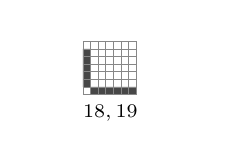
\begin{tikzpicture}[x=1mm,y=1mm,baseline=0mm]
\path[use as bounding box] (0,-.7) rectangle (21.5,11.9);
\begin{scope}[shift={(7.0,3.4)},x=0.97mm,y=0.97mm]
\fill[black!72] (0,5) rectangle (1,6) (0,4) rectangle (1,5) (0,3) rectangle (1,4) (0,2) rectangle (1,3) (0,1) rectangle (1,2) (1,0) rectangle (2,1) (2,0) rectangle (3,1) (3,0) rectangle (4,1) (4,0) rectangle (5,1) (5,0) rectangle (6,1) (6,0) rectangle (7,1);
\draw[black!47,line width=.16pt] (0,0)--(0,7) (0,0)--(7,0) (1,0)--(1,7) (0,1)--(7,1) (2,0)--(2,7) (0,2)--(7,2) (3,0)--(3,7) (0,3)--(7,3) (4,0)--(4,7) (0,4)--(7,4) (5,0)--(5,7) (0,5)--(7,5) (6,0)--(6,7) (0,6)--(7,6) (7,0)--(7,7) (0,7)--(7,7);
\end{scope}
\node[inner sep=0pt,font=\scriptsize] at (10.5,1.1) {$18,19$};
\end{tikzpicture} &
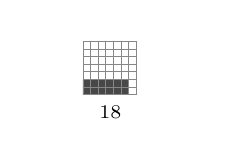
\begin{tikzpicture}[x=1mm,y=1mm,baseline=0mm]
\path[use as bounding box] (0,-.7) rectangle (21.5,11.9);
\begin{scope}[shift={(7.0,3.4)},x=0.97mm,y=0.97mm]
\fill[black!72] (0,1) rectangle (1,2) (1,1) rectangle (2,2) (2,1) rectangle (3,2) (3,1) rectangle (4,2) (4,1) rectangle (5,2) (5,1) rectangle (6,2) (0,0) rectangle (1,1) (1,0) rectangle (2,1) (2,0) rectangle (3,1) (3,0) rectangle (4,1) (4,0) rectangle (5,1) (5,0) rectangle (6,1);
\draw[black!47,line width=.16pt] (0,0)--(0,7) (0,0)--(7,0) (1,0)--(1,7) (0,1)--(7,1) (2,0)--(2,7) (0,2)--(7,2) (3,0)--(3,7) (0,3)--(7,3) (4,0)--(4,7) (0,4)--(7,4) (5,0)--(5,7) (0,5)--(7,5) (6,0)--(6,7) (0,6)--(7,6) (7,0)--(7,7) (0,7)--(7,7);
\end{scope}
\node[inner sep=0pt,font=\scriptsize] at (10.5,1.1) {$18$};
\end{tikzpicture} &
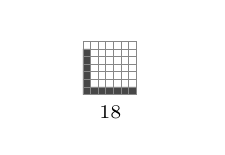
\begin{tikzpicture}[x=1mm,y=1mm,baseline=0mm]
\path[use as bounding box] (0,-.7) rectangle (21.5,11.9);
\begin{scope}[shift={(7.0,3.4)},x=0.97mm,y=0.97mm]
\fill[black!72] (0,5) rectangle (1,6) (0,4) rectangle (1,5) (0,3) rectangle (1,4) (0,2) rectangle (1,3) (0,1) rectangle (1,2) (0,0) rectangle (1,1) (1,0) rectangle (2,1) (2,0) rectangle (3,1) (3,0) rectangle (4,1) (4,0) rectangle (5,1) (5,0) rectangle (6,1) (6,0) rectangle (7,1);
\draw[black!47,line width=.16pt] (0,0)--(0,7) (0,0)--(7,0) (1,0)--(1,7) (0,1)--(7,1) (2,0)--(2,7) (0,2)--(7,2) (3,0)--(3,7) (0,3)--(7,3) (4,0)--(4,7) (0,4)--(7,4) (5,0)--(5,7) (0,5)--(7,5) (6,0)--(6,7) (0,6)--(7,6) (7,0)--(7,7) (0,7)--(7,7);
\end{scope}
\node[inner sep=0pt,font=\scriptsize] at (10.5,1.1) {$18$};
\end{tikzpicture} &
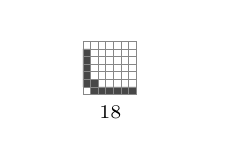
\begin{tikzpicture}[x=1mm,y=1mm,baseline=0mm]
\path[use as bounding box] (0,-.7) rectangle (21.5,11.9);
\begin{scope}[shift={(7.0,3.4)},x=0.97mm,y=0.97mm]
\fill[black!72] (0,5) rectangle (1,6) (0,4) rectangle (1,5) (0,3) rectangle (1,4) (0,2) rectangle (1,3) (0,1) rectangle (1,2) (1,1) rectangle (2,2) (1,0) rectangle (2,1) (2,0) rectangle (3,1) (3,0) rectangle (4,1) (4,0) rectangle (5,1) (5,0) rectangle (6,1) (6,0) rectangle (7,1);
\draw[black!47,line width=.16pt] (0,0)--(0,7) (0,0)--(7,0) (1,0)--(1,7) (0,1)--(7,1) (2,0)--(2,7) (0,2)--(7,2) (3,0)--(3,7) (0,3)--(7,3) (4,0)--(4,7) (0,4)--(7,4) (5,0)--(5,7) (0,5)--(7,5) (6,0)--(6,7) (0,6)--(7,6) (7,0)--(7,7) (0,7)--(7,7);
\end{scope}
\node[inner sep=0pt,font=\scriptsize] at (10.5,1.1) {$18$};
\end{tikzpicture} &
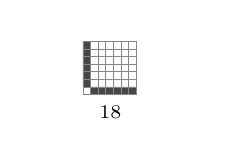
\begin{tikzpicture}[x=1mm,y=1mm,baseline=0mm]
\path[use as bounding box] (0,-.7) rectangle (21.5,11.9);
\begin{scope}[shift={(7.0,3.4)},x=0.97mm,y=0.97mm]
\fill[black!72] (0,6) rectangle (1,7) (0,5) rectangle (1,6) (0,4) rectangle (1,5) (0,3) rectangle (1,4) (0,2) rectangle (1,3) (0,1) rectangle (1,2) (1,0) rectangle (2,1) (2,0) rectangle (3,1) (3,0) rectangle (4,1) (4,0) rectangle (5,1) (5,0) rectangle (6,1) (6,0) rectangle (7,1);
\draw[black!47,line width=.16pt] (0,0)--(0,7) (0,0)--(7,0) (1,0)--(1,7) (0,1)--(7,1) (2,0)--(2,7) (0,2)--(7,2) (3,0)--(3,7) (0,3)--(7,3) (4,0)--(4,7) (0,4)--(7,4) (5,0)--(5,7) (0,5)--(7,5) (6,0)--(6,7) (0,6)--(7,6) (7,0)--(7,7) (0,7)--(7,7);
\end{scope}
\node[inner sep=0pt,font=\scriptsize] at (10.5,1.1) {$18$};
\end{tikzpicture} \\[.4mm]
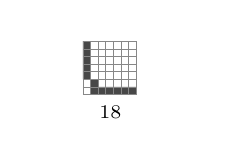
\begin{tikzpicture}[x=1mm,y=1mm,baseline=0mm]
\path[use as bounding box] (0,-.7) rectangle (21.5,11.9);
\begin{scope}[shift={(7.0,3.4)},x=0.97mm,y=0.97mm]
\fill[black!72] (0,6) rectangle (1,7) (0,5) rectangle (1,6) (0,4) rectangle (1,5) (0,3) rectangle (1,4) (0,2) rectangle (1,3) (1,1) rectangle (2,2) (1,0) rectangle (2,1) (2,0) rectangle (3,1) (3,0) rectangle (4,1) (4,0) rectangle (5,1) (5,0) rectangle (6,1) (6,0) rectangle (7,1);
\draw[black!47,line width=.16pt] (0,0)--(0,7) (0,0)--(7,0) (1,0)--(1,7) (0,1)--(7,1) (2,0)--(2,7) (0,2)--(7,2) (3,0)--(3,7) (0,3)--(7,3) (4,0)--(4,7) (0,4)--(7,4) (5,0)--(5,7) (0,5)--(7,5) (6,0)--(6,7) (0,6)--(7,6) (7,0)--(7,7) (0,7)--(7,7);
\end{scope}
\node[inner sep=0pt,font=\scriptsize] at (10.5,1.1) {$18$};
\end{tikzpicture} &
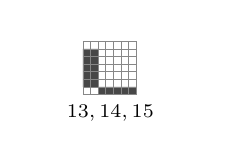
\begin{tikzpicture}[x=1mm,y=1mm,baseline=0mm]
\path[use as bounding box] (0,-.7) rectangle (21.5,11.9);
\begin{scope}[shift={(7.0,3.4)},x=0.97mm,y=0.97mm]
\fill[black!72] (0,5) rectangle (1,6) (1,5) rectangle (2,6) (0,4) rectangle (1,5) (1,4) rectangle (2,5) (0,3) rectangle (1,4) (1,3) rectangle (2,4) (0,2) rectangle (1,3) (1,2) rectangle (2,3) (0,1) rectangle (1,2) (1,1) rectangle (2,2) (2,0) rectangle (3,1) (3,0) rectangle (4,1) (4,0) rectangle (5,1) (5,0) rectangle (6,1) (6,0) rectangle (7,1);
\draw[black!47,line width=.16pt] (0,0)--(0,7) (0,0)--(7,0) (1,0)--(1,7) (0,1)--(7,1) (2,0)--(2,7) (0,2)--(7,2) (3,0)--(3,7) (0,3)--(7,3) (4,0)--(4,7) (0,4)--(7,4) (5,0)--(5,7) (0,5)--(7,5) (6,0)--(6,7) (0,6)--(7,6) (7,0)--(7,7) (0,7)--(7,7);
\end{scope}
\node[inner sep=0pt,font=\scriptsize] at (10.5,1.1) {$13,14,15$};
\end{tikzpicture} &
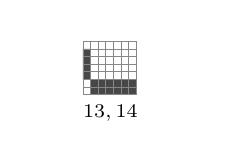
\begin{tikzpicture}[x=1mm,y=1mm,baseline=0mm]
\path[use as bounding box] (0,-.7) rectangle (21.5,11.9);
\begin{scope}[shift={(7.0,3.4)},x=0.97mm,y=0.97mm]
\fill[black!72] (0,5) rectangle (1,6) (0,4) rectangle (1,5) (0,3) rectangle (1,4) (0,2) rectangle (1,3) (1,1) rectangle (2,2) (2,1) rectangle (3,2) (3,1) rectangle (4,2) (4,1) rectangle (5,2) (5,1) rectangle (6,2) (6,1) rectangle (7,2) (1,0) rectangle (2,1) (2,0) rectangle (3,1) (3,0) rectangle (4,1) (4,0) rectangle (5,1) (5,0) rectangle (6,1) (6,0) rectangle (7,1);
\draw[black!47,line width=.16pt] (0,0)--(0,7) (0,0)--(7,0) (1,0)--(1,7) (0,1)--(7,1) (2,0)--(2,7) (0,2)--(7,2) (3,0)--(3,7) (0,3)--(7,3) (4,0)--(4,7) (0,4)--(7,4) (5,0)--(5,7) (0,5)--(7,5) (6,0)--(6,7) (0,6)--(7,6) (7,0)--(7,7) (0,7)--(7,7);
\end{scope}
\node[inner sep=0pt,font=\scriptsize] at (10.5,1.1) {$13,14$};
\end{tikzpicture} &
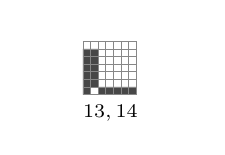
\begin{tikzpicture}[x=1mm,y=1mm,baseline=0mm]
\path[use as bounding box] (0,-.7) rectangle (21.5,11.9);
\begin{scope}[shift={(7.0,3.4)},x=0.97mm,y=0.97mm]
\fill[black!72] (0,5) rectangle (1,6) (1,5) rectangle (2,6) (0,4) rectangle (1,5) (1,4) rectangle (2,5) (0,3) rectangle (1,4) (1,3) rectangle (2,4) (0,2) rectangle (1,3) (1,2) rectangle (2,3) (0,1) rectangle (1,2) (1,1) rectangle (2,2) (0,0) rectangle (1,1) (2,0) rectangle (3,1) (3,0) rectangle (4,1) (4,0) rectangle (5,1) (5,0) rectangle (6,1) (6,0) rectangle (7,1);
\draw[black!47,line width=.16pt] (0,0)--(0,7) (0,0)--(7,0) (1,0)--(1,7) (0,1)--(7,1) (2,0)--(2,7) (0,2)--(7,2) (3,0)--(3,7) (0,3)--(7,3) (4,0)--(4,7) (0,4)--(7,4) (5,0)--(5,7) (0,5)--(7,5) (6,0)--(6,7) (0,6)--(7,6) (7,0)--(7,7) (0,7)--(7,7);
\end{scope}
\node[inner sep=0pt,font=\scriptsize] at (10.5,1.1) {$13,14$};
\end{tikzpicture} &
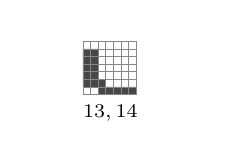
\begin{tikzpicture}[x=1mm,y=1mm,baseline=0mm]
\path[use as bounding box] (0,-.7) rectangle (21.5,11.9);
\begin{scope}[shift={(7.0,3.4)},x=0.97mm,y=0.97mm]
\fill[black!72] (0,5) rectangle (1,6) (1,5) rectangle (2,6) (0,4) rectangle (1,5) (1,4) rectangle (2,5) (0,3) rectangle (1,4) (1,3) rectangle (2,4) (0,2) rectangle (1,3) (1,2) rectangle (2,3) (0,1) rectangle (1,2) (1,1) rectangle (2,2) (2,1) rectangle (3,2) (2,0) rectangle (3,1) (3,0) rectangle (4,1) (4,0) rectangle (5,1) (5,0) rectangle (6,1) (6,0) rectangle (7,1);
\draw[black!47,line width=.16pt] (0,0)--(0,7) (0,0)--(7,0) (1,0)--(1,7) (0,1)--(7,1) (2,0)--(2,7) (0,2)--(7,2) (3,0)--(3,7) (0,3)--(7,3) (4,0)--(4,7) (0,4)--(7,4) (5,0)--(5,7) (0,5)--(7,5) (6,0)--(6,7) (0,6)--(7,6) (7,0)--(7,7) (0,7)--(7,7);
\end{scope}
\node[inner sep=0pt,font=\scriptsize] at (10.5,1.1) {$13,14$};
\end{tikzpicture} \\[.4mm]
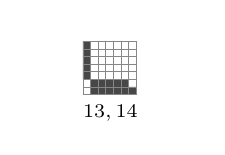
\begin{tikzpicture}[x=1mm,y=1mm,baseline=0mm]
\path[use as bounding box] (0,-.7) rectangle (21.5,11.9);
\begin{scope}[shift={(7.0,3.4)},x=0.97mm,y=0.97mm]
\fill[black!72] (0,6) rectangle (1,7) (0,5) rectangle (1,6) (0,4) rectangle (1,5) (0,3) rectangle (1,4) (0,2) rectangle (1,3) (1,1) rectangle (2,2) (2,1) rectangle (3,2) (3,1) rectangle (4,2) (4,1) rectangle (5,2) (5,1) rectangle (6,2) (1,0) rectangle (2,1) (2,0) rectangle (3,1) (3,0) rectangle (4,1) (4,0) rectangle (5,1) (5,0) rectangle (6,1) (6,0) rectangle (7,1);
\draw[black!47,line width=.16pt] (0,0)--(0,7) (0,0)--(7,0) (1,0)--(1,7) (0,1)--(7,1) (2,0)--(2,7) (0,2)--(7,2) (3,0)--(3,7) (0,3)--(7,3) (4,0)--(4,7) (0,4)--(7,4) (5,0)--(5,7) (0,5)--(7,5) (6,0)--(6,7) (0,6)--(7,6) (7,0)--(7,7) (0,7)--(7,7);
\end{scope}
\node[inner sep=0pt,font=\scriptsize] at (10.5,1.1) {$13,14$};
\end{tikzpicture} &
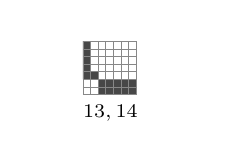
\begin{tikzpicture}[x=1mm,y=1mm,baseline=0mm]
\path[use as bounding box] (0,-.7) rectangle (21.5,11.9);
\begin{scope}[shift={(7.0,3.4)},x=0.97mm,y=0.97mm]
\fill[black!72] (0,6) rectangle (1,7) (0,5) rectangle (1,6) (0,4) rectangle (1,5) (0,3) rectangle (1,4) (0,2) rectangle (1,3) (1,2) rectangle (2,3) (2,1) rectangle (3,2) (3,1) rectangle (4,2) (4,1) rectangle (5,2) (5,1) rectangle (6,2) (6,1) rectangle (7,2) (2,0) rectangle (3,1) (3,0) rectangle (4,1) (4,0) rectangle (5,1) (5,0) rectangle (6,1) (6,0) rectangle (7,1);
\draw[black!47,line width=.16pt] (0,0)--(0,7) (0,0)--(7,0) (1,0)--(1,7) (0,1)--(7,1) (2,0)--(2,7) (0,2)--(7,2) (3,0)--(3,7) (0,3)--(7,3) (4,0)--(4,7) (0,4)--(7,4) (5,0)--(5,7) (0,5)--(7,5) (6,0)--(6,7) (0,6)--(7,6) (7,0)--(7,7) (0,7)--(7,7);
\end{scope}
\node[inner sep=0pt,font=\scriptsize] at (10.5,1.1) {$13,14$};
\end{tikzpicture} &
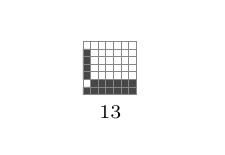
\begin{tikzpicture}[x=1mm,y=1mm,baseline=0mm]
\path[use as bounding box] (0,-.7) rectangle (21.5,11.9);
\begin{scope}[shift={(7.0,3.4)},x=0.97mm,y=0.97mm]
\fill[black!72] (0,5) rectangle (1,6) (0,4) rectangle (1,5) (0,3) rectangle (1,4) (0,2) rectangle (1,3) (1,1) rectangle (2,2) (2,1) rectangle (3,2) (3,1) rectangle (4,2) (4,1) rectangle (5,2) (5,1) rectangle (6,2) (6,1) rectangle (7,2) (0,0) rectangle (1,1) (1,0) rectangle (2,1) (2,0) rectangle (3,1) (3,0) rectangle (4,1) (4,0) rectangle (5,1) (5,0) rectangle (6,1) (6,0) rectangle (7,1);
\draw[black!47,line width=.16pt] (0,0)--(0,7) (0,0)--(7,0) (1,0)--(1,7) (0,1)--(7,1) (2,0)--(2,7) (0,2)--(7,2) (3,0)--(3,7) (0,3)--(7,3) (4,0)--(4,7) (0,4)--(7,4) (5,0)--(5,7) (0,5)--(7,5) (6,0)--(6,7) (0,6)--(7,6) (7,0)--(7,7) (0,7)--(7,7);
\end{scope}
\node[inner sep=0pt,font=\scriptsize] at (10.5,1.1) {$13$};
\end{tikzpicture} &
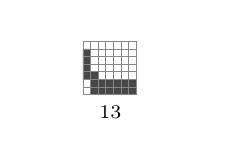
\begin{tikzpicture}[x=1mm,y=1mm,baseline=0mm]
\path[use as bounding box] (0,-.7) rectangle (21.5,11.9);
\begin{scope}[shift={(7.0,3.4)},x=0.97mm,y=0.97mm]
\fill[black!72] (0,5) rectangle (1,6) (0,4) rectangle (1,5) (0,3) rectangle (1,4) (0,2) rectangle (1,3) (1,2) rectangle (2,3) (1,1) rectangle (2,2) (2,1) rectangle (3,2) (3,1) rectangle (4,2) (4,1) rectangle (5,2) (5,1) rectangle (6,2) (6,1) rectangle (7,2) (1,0) rectangle (2,1) (2,0) rectangle (3,1) (3,0) rectangle (4,1) (4,0) rectangle (5,1) (5,0) rectangle (6,1) (6,0) rectangle (7,1);
\draw[black!47,line width=.16pt] (0,0)--(0,7) (0,0)--(7,0) (1,0)--(1,7) (0,1)--(7,1) (2,0)--(2,7) (0,2)--(7,2) (3,0)--(3,7) (0,3)--(7,3) (4,0)--(4,7) (0,4)--(7,4) (5,0)--(5,7) (0,5)--(7,5) (6,0)--(6,7) (0,6)--(7,6) (7,0)--(7,7) (0,7)--(7,7);
\end{scope}
\node[inner sep=0pt,font=\scriptsize] at (10.5,1.1) {$13$};
\end{tikzpicture} &
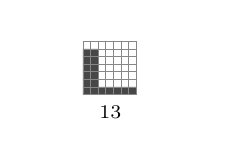
\begin{tikzpicture}[x=1mm,y=1mm,baseline=0mm]
\path[use as bounding box] (0,-.7) rectangle (21.5,11.9);
\begin{scope}[shift={(7.0,3.4)},x=0.97mm,y=0.97mm]
\fill[black!72] (0,5) rectangle (1,6) (1,5) rectangle (2,6) (0,4) rectangle (1,5) (1,4) rectangle (2,5) (0,3) rectangle (1,4) (1,3) rectangle (2,4) (0,2) rectangle (1,3) (1,2) rectangle (2,3) (0,1) rectangle (1,2) (1,1) rectangle (2,2) (0,0) rectangle (1,1) (1,0) rectangle (2,1) (2,0) rectangle (3,1) (3,0) rectangle (4,1) (4,0) rectangle (5,1) (5,0) rectangle (6,1) (6,0) rectangle (7,1);
\draw[black!47,line width=.16pt] (0,0)--(0,7) (0,0)--(7,0) (1,0)--(1,7) (0,1)--(7,1) (2,0)--(2,7) (0,2)--(7,2) (3,0)--(3,7) (0,3)--(7,3) (4,0)--(4,7) (0,4)--(7,4) (5,0)--(5,7) (0,5)--(7,5) (6,0)--(6,7) (0,6)--(7,6) (7,0)--(7,7) (0,7)--(7,7);
\end{scope}
\node[inner sep=0pt,font=\scriptsize] at (10.5,1.1) {$13$};
\end{tikzpicture} \\[.4mm]
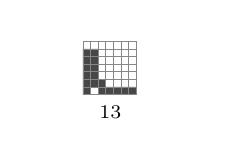
\begin{tikzpicture}[x=1mm,y=1mm,baseline=0mm]
\path[use as bounding box] (0,-.7) rectangle (21.5,11.9);
\begin{scope}[shift={(7.0,3.4)},x=0.97mm,y=0.97mm]
\fill[black!72] (0,5) rectangle (1,6) (1,5) rectangle (2,6) (0,4) rectangle (1,5) (1,4) rectangle (2,5) (0,3) rectangle (1,4) (1,3) rectangle (2,4) (0,2) rectangle (1,3) (1,2) rectangle (2,3) (0,1) rectangle (1,2) (1,1) rectangle (2,2) (2,1) rectangle (3,2) (0,0) rectangle (1,1) (2,0) rectangle (3,1) (3,0) rectangle (4,1) (4,0) rectangle (5,1) (5,0) rectangle (6,1) (6,0) rectangle (7,1);
\draw[black!47,line width=.16pt] (0,0)--(0,7) (0,0)--(7,0) (1,0)--(1,7) (0,1)--(7,1) (2,0)--(2,7) (0,2)--(7,2) (3,0)--(3,7) (0,3)--(7,3) (4,0)--(4,7) (0,4)--(7,4) (5,0)--(5,7) (0,5)--(7,5) (6,0)--(6,7) (0,6)--(7,6) (7,0)--(7,7) (0,7)--(7,7);
\end{scope}
\node[inner sep=0pt,font=\scriptsize] at (10.5,1.1) {$13$};
\end{tikzpicture} &
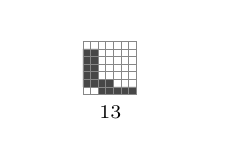
\begin{tikzpicture}[x=1mm,y=1mm,baseline=0mm]
\path[use as bounding box] (0,-.7) rectangle (21.5,11.9);
\begin{scope}[shift={(7.0,3.4)},x=0.97mm,y=0.97mm]
\fill[black!72] (0,5) rectangle (1,6) (1,5) rectangle (2,6) (0,4) rectangle (1,5) (1,4) rectangle (2,5) (0,3) rectangle (1,4) (1,3) rectangle (2,4) (0,2) rectangle (1,3) (1,2) rectangle (2,3) (0,1) rectangle (1,2) (1,1) rectangle (2,2) (2,1) rectangle (3,2) (3,1) rectangle (4,2) (2,0) rectangle (3,1) (3,0) rectangle (4,1) (4,0) rectangle (5,1) (5,0) rectangle (6,1) (6,0) rectangle (7,1);
\draw[black!47,line width=.16pt] (0,0)--(0,7) (0,0)--(7,0) (1,0)--(1,7) (0,1)--(7,1) (2,0)--(2,7) (0,2)--(7,2) (3,0)--(3,7) (0,3)--(7,3) (4,0)--(4,7) (0,4)--(7,4) (5,0)--(5,7) (0,5)--(7,5) (6,0)--(6,7) (0,6)--(7,6) (7,0)--(7,7) (0,7)--(7,7);
\end{scope}
\node[inner sep=0pt,font=\scriptsize] at (10.5,1.1) {$13$};
\end{tikzpicture} &
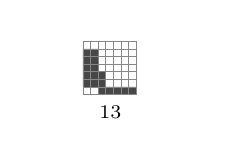
\begin{tikzpicture}[x=1mm,y=1mm,baseline=0mm]
\path[use as bounding box] (0,-.7) rectangle (21.5,11.9);
\begin{scope}[shift={(7.0,3.4)},x=0.97mm,y=0.97mm]
\fill[black!72] (0,5) rectangle (1,6) (1,5) rectangle (2,6) (0,4) rectangle (1,5) (1,4) rectangle (2,5) (0,3) rectangle (1,4) (1,3) rectangle (2,4) (0,2) rectangle (1,3) (1,2) rectangle (2,3) (2,2) rectangle (3,3) (0,1) rectangle (1,2) (1,1) rectangle (2,2) (2,1) rectangle (3,2) (2,0) rectangle (3,1) (3,0) rectangle (4,1) (4,0) rectangle (5,1) (5,0) rectangle (6,1) (6,0) rectangle (7,1);
\draw[black!47,line width=.16pt] (0,0)--(0,7) (0,0)--(7,0) (1,0)--(1,7) (0,1)--(7,1) (2,0)--(2,7) (0,2)--(7,2) (3,0)--(3,7) (0,3)--(7,3) (4,0)--(4,7) (0,4)--(7,4) (5,0)--(5,7) (0,5)--(7,5) (6,0)--(6,7) (0,6)--(7,6) (7,0)--(7,7) (0,7)--(7,7);
\end{scope}
\node[inner sep=0pt,font=\scriptsize] at (10.5,1.1) {$13$};
\end{tikzpicture} &
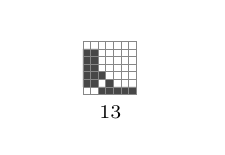
\begin{tikzpicture}[x=1mm,y=1mm,baseline=0mm]
\path[use as bounding box] (0,-.7) rectangle (21.5,11.9);
\begin{scope}[shift={(7.0,3.4)},x=0.97mm,y=0.97mm]
\fill[black!72] (0,5) rectangle (1,6) (1,5) rectangle (2,6) (0,4) rectangle (1,5) (1,4) rectangle (2,5) (0,3) rectangle (1,4) (1,3) rectangle (2,4) (0,2) rectangle (1,3) (1,2) rectangle (2,3) (2,2) rectangle (3,3) (0,1) rectangle (1,2) (1,1) rectangle (2,2) (3,1) rectangle (4,2) (2,0) rectangle (3,1) (3,0) rectangle (4,1) (4,0) rectangle (5,1) (5,0) rectangle (6,1) (6,0) rectangle (7,1);
\draw[black!47,line width=.16pt] (0,0)--(0,7) (0,0)--(7,0) (1,0)--(1,7) (0,1)--(7,1) (2,0)--(2,7) (0,2)--(7,2) (3,0)--(3,7) (0,3)--(7,3) (4,0)--(4,7) (0,4)--(7,4) (5,0)--(5,7) (0,5)--(7,5) (6,0)--(6,7) (0,6)--(7,6) (7,0)--(7,7) (0,7)--(7,7);
\end{scope}
\node[inner sep=0pt,font=\scriptsize] at (10.5,1.1) {$13$};
\end{tikzpicture} &
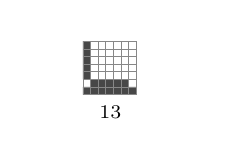
\begin{tikzpicture}[x=1mm,y=1mm,baseline=0mm]
\path[use as bounding box] (0,-.7) rectangle (21.5,11.9);
\begin{scope}[shift={(7.0,3.4)},x=0.97mm,y=0.97mm]
\fill[black!72] (0,6) rectangle (1,7) (0,5) rectangle (1,6) (0,4) rectangle (1,5) (0,3) rectangle (1,4) (0,2) rectangle (1,3) (1,1) rectangle (2,2) (2,1) rectangle (3,2) (3,1) rectangle (4,2) (4,1) rectangle (5,2) (5,1) rectangle (6,2) (0,0) rectangle (1,1) (1,0) rectangle (2,1) (2,0) rectangle (3,1) (3,0) rectangle (4,1) (4,0) rectangle (5,1) (5,0) rectangle (6,1) (6,0) rectangle (7,1);
\draw[black!47,line width=.16pt] (0,0)--(0,7) (0,0)--(7,0) (1,0)--(1,7) (0,1)--(7,1) (2,0)--(2,7) (0,2)--(7,2) (3,0)--(3,7) (0,3)--(7,3) (4,0)--(4,7) (0,4)--(7,4) (5,0)--(5,7) (0,5)--(7,5) (6,0)--(6,7) (0,6)--(7,6) (7,0)--(7,7) (0,7)--(7,7);
\end{scope}
\node[inner sep=0pt,font=\scriptsize] at (10.5,1.1) {$13$};
\end{tikzpicture} \\[.4mm]
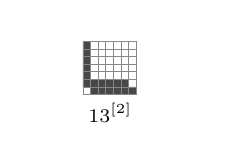
\begin{tikzpicture}[x=1mm,y=1mm,baseline=0mm]
\path[use as bounding box] (0,-.7) rectangle (21.5,11.9);
\begin{scope}[shift={(7.0,3.4)},x=0.97mm,y=0.97mm]
\fill[black!72] (0,6) rectangle (1,7) (0,5) rectangle (1,6) (0,4) rectangle (1,5) (0,3) rectangle (1,4) (0,2) rectangle (1,3) (0,1) rectangle (1,2) (1,1) rectangle (2,2) (2,1) rectangle (3,2) (3,1) rectangle (4,2) (4,1) rectangle (5,2) (5,1) rectangle (6,2) (1,0) rectangle (2,1) (2,0) rectangle (3,1) (3,0) rectangle (4,1) (4,0) rectangle (5,1) (5,0) rectangle (6,1) (6,0) rectangle (7,1);
\draw[black!47,line width=.16pt] (0,0)--(0,7) (0,0)--(7,0) (1,0)--(1,7) (0,1)--(7,1) (2,0)--(2,7) (0,2)--(7,2) (3,0)--(3,7) (0,3)--(7,3) (4,0)--(4,7) (0,4)--(7,4) (5,0)--(5,7) (0,5)--(7,5) (6,0)--(6,7) (0,6)--(7,6) (7,0)--(7,7) (0,7)--(7,7);
\end{scope}
\node[inner sep=0pt,font=\scriptsize] at (10.5,1.1) {$13^{[2]}$};
\end{tikzpicture} &
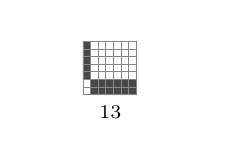
\begin{tikzpicture}[x=1mm,y=1mm,baseline=0mm]
\path[use as bounding box] (0,-.7) rectangle (21.5,11.9);
\begin{scope}[shift={(7.0,3.4)},x=0.97mm,y=0.97mm]
\fill[black!72] (0,6) rectangle (1,7) (0,5) rectangle (1,6) (0,4) rectangle (1,5) (0,3) rectangle (1,4) (0,2) rectangle (1,3) (1,1) rectangle (2,2) (2,1) rectangle (3,2) (3,1) rectangle (4,2) (4,1) rectangle (5,2) (5,1) rectangle (6,2) (6,1) rectangle (7,2) (1,0) rectangle (2,1) (2,0) rectangle (3,1) (3,0) rectangle (4,1) (4,0) rectangle (5,1) (5,0) rectangle (6,1) (6,0) rectangle (7,1);
\draw[black!47,line width=.16pt] (0,0)--(0,7) (0,0)--(7,0) (1,0)--(1,7) (0,1)--(7,1) (2,0)--(2,7) (0,2)--(7,2) (3,0)--(3,7) (0,3)--(7,3) (4,0)--(4,7) (0,4)--(7,4) (5,0)--(5,7) (0,5)--(7,5) (6,0)--(6,7) (0,6)--(7,6) (7,0)--(7,7) (0,7)--(7,7);
\end{scope}
\node[inner sep=0pt,font=\scriptsize] at (10.5,1.1) {$13$};
\end{tikzpicture} &
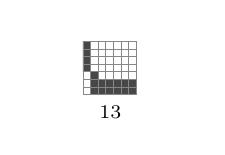
\begin{tikzpicture}[x=1mm,y=1mm,baseline=0mm]
\path[use as bounding box] (0,-.7) rectangle (21.5,11.9);
\begin{scope}[shift={(7.0,3.4)},x=0.97mm,y=0.97mm]
\fill[black!72] (0,6) rectangle (1,7) (0,5) rectangle (1,6) (0,4) rectangle (1,5) (0,3) rectangle (1,4) (1,2) rectangle (2,3) (1,1) rectangle (2,2) (2,1) rectangle (3,2) (3,1) rectangle (4,2) (4,1) rectangle (5,2) (5,1) rectangle (6,2) (6,1) rectangle (7,2) (1,0) rectangle (2,1) (2,0) rectangle (3,1) (3,0) rectangle (4,1) (4,0) rectangle (5,1) (5,0) rectangle (6,1) (6,0) rectangle (7,1);
\draw[black!47,line width=.16pt] (0,0)--(0,7) (0,0)--(7,0) (1,0)--(1,7) (0,1)--(7,1) (2,0)--(2,7) (0,2)--(7,2) (3,0)--(3,7) (0,3)--(7,3) (4,0)--(4,7) (0,4)--(7,4) (5,0)--(5,7) (0,5)--(7,5) (6,0)--(6,7) (0,6)--(7,6) (7,0)--(7,7) (0,7)--(7,7);
\end{scope}
\node[inner sep=0pt,font=\scriptsize] at (10.5,1.1) {$13$};
\end{tikzpicture} &
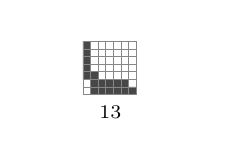
\begin{tikzpicture}[x=1mm,y=1mm,baseline=0mm]
\path[use as bounding box] (0,-.7) rectangle (21.5,11.9);
\begin{scope}[shift={(7.0,3.4)},x=0.97mm,y=0.97mm]
\fill[black!72] (0,6) rectangle (1,7) (0,5) rectangle (1,6) (0,4) rectangle (1,5) (0,3) rectangle (1,4) (0,2) rectangle (1,3) (1,2) rectangle (2,3) (1,1) rectangle (2,2) (2,1) rectangle (3,2) (3,1) rectangle (4,2) (4,1) rectangle (5,2) (5,1) rectangle (6,2) (1,0) rectangle (2,1) (2,0) rectangle (3,1) (3,0) rectangle (4,1) (4,0) rectangle (5,1) (5,0) rectangle (6,1) (6,0) rectangle (7,1);
\draw[black!47,line width=.16pt] (0,0)--(0,7) (0,0)--(7,0) (1,0)--(1,7) (0,1)--(7,1) (2,0)--(2,7) (0,2)--(7,2) (3,0)--(3,7) (0,3)--(7,3) (4,0)--(4,7) (0,4)--(7,4) (5,0)--(5,7) (0,5)--(7,5) (6,0)--(6,7) (0,6)--(7,6) (7,0)--(7,7) (0,7)--(7,7);
\end{scope}
\node[inner sep=0pt,font=\scriptsize] at (10.5,1.1) {$13$};
\end{tikzpicture} &
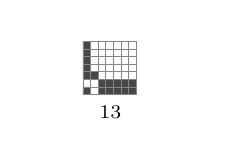
\begin{tikzpicture}[x=1mm,y=1mm,baseline=0mm]
\path[use as bounding box] (0,-.7) rectangle (21.5,11.9);
\begin{scope}[shift={(7.0,3.4)},x=0.97mm,y=0.97mm]
\fill[black!72] (0,6) rectangle (1,7) (0,5) rectangle (1,6) (0,4) rectangle (1,5) (0,3) rectangle (1,4) (0,2) rectangle (1,3) (1,2) rectangle (2,3) (2,1) rectangle (3,2) (3,1) rectangle (4,2) (4,1) rectangle (5,2) (5,1) rectangle (6,2) (6,1) rectangle (7,2) (0,0) rectangle (1,1) (2,0) rectangle (3,1) (3,0) rectangle (4,1) (4,0) rectangle (5,1) (5,0) rectangle (6,1) (6,0) rectangle (7,1);
\draw[black!47,line width=.16pt] (0,0)--(0,7) (0,0)--(7,0) (1,0)--(1,7) (0,1)--(7,1) (2,0)--(2,7) (0,2)--(7,2) (3,0)--(3,7) (0,3)--(7,3) (4,0)--(4,7) (0,4)--(7,4) (5,0)--(5,7) (0,5)--(7,5) (6,0)--(6,7) (0,6)--(7,6) (7,0)--(7,7) (0,7)--(7,7);
\end{scope}
\node[inner sep=0pt,font=\scriptsize] at (10.5,1.1) {$13$};
\end{tikzpicture} \\[.4mm]
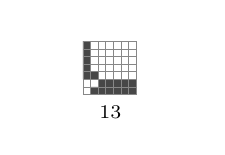
\begin{tikzpicture}[x=1mm,y=1mm,baseline=0mm]
\path[use as bounding box] (0,-.7) rectangle (21.5,11.9);
\begin{scope}[shift={(7.0,3.4)},x=0.97mm,y=0.97mm]
\fill[black!72] (0,6) rectangle (1,7) (0,5) rectangle (1,6) (0,4) rectangle (1,5) (0,3) rectangle (1,4) (0,2) rectangle (1,3) (1,2) rectangle (2,3) (2,1) rectangle (3,2) (3,1) rectangle (4,2) (4,1) rectangle (5,2) (5,1) rectangle (6,2) (6,1) rectangle (7,2) (1,0) rectangle (2,1) (2,0) rectangle (3,1) (3,0) rectangle (4,1) (4,0) rectangle (5,1) (5,0) rectangle (6,1) (6,0) rectangle (7,1);
\draw[black!47,line width=.16pt] (0,0)--(0,7) (0,0)--(7,0) (1,0)--(1,7) (0,1)--(7,1) (2,0)--(2,7) (0,2)--(7,2) (3,0)--(3,7) (0,3)--(7,3) (4,0)--(4,7) (0,4)--(7,4) (5,0)--(5,7) (0,5)--(7,5) (6,0)--(6,7) (0,6)--(7,6) (7,0)--(7,7) (0,7)--(7,7);
\end{scope}
\node[inner sep=0pt,font=\scriptsize] at (10.5,1.1) {$13$};
\end{tikzpicture} &
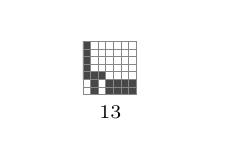
\begin{tikzpicture}[x=1mm,y=1mm,baseline=0mm]
\path[use as bounding box] (0,-.7) rectangle (21.5,11.9);
\begin{scope}[shift={(7.0,3.4)},x=0.97mm,y=0.97mm]
\fill[black!72] (0,6) rectangle (1,7) (0,5) rectangle (1,6) (0,4) rectangle (1,5) (0,3) rectangle (1,4) (0,2) rectangle (1,3) (1,2) rectangle (2,3) (2,2) rectangle (3,3) (1,1) rectangle (2,2) (3,1) rectangle (4,2) (4,1) rectangle (5,2) (5,1) rectangle (6,2) (6,1) rectangle (7,2) (1,0) rectangle (2,1) (3,0) rectangle (4,1) (4,0) rectangle (5,1) (5,0) rectangle (6,1) (6,0) rectangle (7,1);
\draw[black!47,line width=.16pt] (0,0)--(0,7) (0,0)--(7,0) (1,0)--(1,7) (0,1)--(7,1) (2,0)--(2,7) (0,2)--(7,2) (3,0)--(3,7) (0,3)--(7,3) (4,0)--(4,7) (0,4)--(7,4) (5,0)--(5,7) (0,5)--(7,5) (6,0)--(6,7) (0,6)--(7,6) (7,0)--(7,7) (0,7)--(7,7);
\end{scope}
\node[inner sep=0pt,font=\scriptsize] at (10.5,1.1) {$13$};
\end{tikzpicture} &
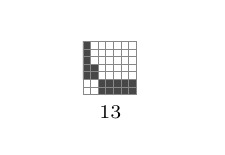
\begin{tikzpicture}[x=1mm,y=1mm,baseline=0mm]
\path[use as bounding box] (0,-.7) rectangle (21.5,11.9);
\begin{scope}[shift={(7.0,3.4)},x=0.97mm,y=0.97mm]
\fill[black!72] (0,6) rectangle (1,7) (0,5) rectangle (1,6) (0,4) rectangle (1,5) (0,3) rectangle (1,4) (1,3) rectangle (2,4) (0,2) rectangle (1,3) (1,2) rectangle (2,3) (2,1) rectangle (3,2) (3,1) rectangle (4,2) (4,1) rectangle (5,2) (5,1) rectangle (6,2) (6,1) rectangle (7,2) (2,0) rectangle (3,1) (3,0) rectangle (4,1) (4,0) rectangle (5,1) (5,0) rectangle (6,1) (6,0) rectangle (7,1);
\draw[black!47,line width=.16pt] (0,0)--(0,7) (0,0)--(7,0) (1,0)--(1,7) (0,1)--(7,1) (2,0)--(2,7) (0,2)--(7,2) (3,0)--(3,7) (0,3)--(7,3) (4,0)--(4,7) (0,4)--(7,4) (5,0)--(5,7) (0,5)--(7,5) (6,0)--(6,7) (0,6)--(7,6) (7,0)--(7,7) (0,7)--(7,7);
\end{scope}
\node[inner sep=0pt,font=\scriptsize] at (10.5,1.1) {$13$};
\end{tikzpicture} &
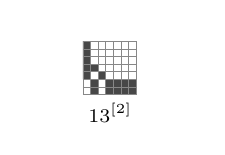
\begin{tikzpicture}[x=1mm,y=1mm,baseline=0mm]
\path[use as bounding box] (0,-.7) rectangle (21.5,11.9);
\begin{scope}[shift={(7.0,3.4)},x=0.97mm,y=0.97mm]
\fill[black!72] (0,6) rectangle (1,7) (0,5) rectangle (1,6) (0,4) rectangle (1,5) (0,3) rectangle (1,4) (1,3) rectangle (2,4) (0,2) rectangle (1,3) (2,2) rectangle (3,3) (1,1) rectangle (2,2) (3,1) rectangle (4,2) (4,1) rectangle (5,2) (5,1) rectangle (6,2) (6,1) rectangle (7,2) (1,0) rectangle (2,1) (3,0) rectangle (4,1) (4,0) rectangle (5,1) (5,0) rectangle (6,1) (6,0) rectangle (7,1);
\draw[black!47,line width=.16pt] (0,0)--(0,7) (0,0)--(7,0) (1,0)--(1,7) (0,1)--(7,1) (2,0)--(2,7) (0,2)--(7,2) (3,0)--(3,7) (0,3)--(7,3) (4,0)--(4,7) (0,4)--(7,4) (5,0)--(5,7) (0,5)--(7,5) (6,0)--(6,7) (0,6)--(7,6) (7,0)--(7,7) (0,7)--(7,7);
\end{scope}
\node[inner sep=0pt,font=\scriptsize] at (10.5,1.1) {$13^{[2]}$};
\end{tikzpicture} &
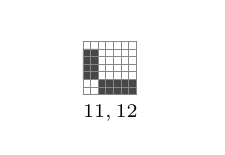
\begin{tikzpicture}[x=1mm,y=1mm,baseline=0mm]
\path[use as bounding box] (0,-.7) rectangle (21.5,11.9);
\begin{scope}[shift={(7.0,3.4)},x=0.97mm,y=0.97mm]
\fill[black!72] (0,5) rectangle (1,6) (1,5) rectangle (2,6) (0,4) rectangle (1,5) (1,4) rectangle (2,5) (0,3) rectangle (1,4) (1,3) rectangle (2,4) (0,2) rectangle (1,3) (1,2) rectangle (2,3) (2,1) rectangle (3,2) (3,1) rectangle (4,2) (4,1) rectangle (5,2) (5,1) rectangle (6,2) (6,1) rectangle (7,2) (2,0) rectangle (3,1) (3,0) rectangle (4,1) (4,0) rectangle (5,1) (5,0) rectangle (6,1) (6,0) rectangle (7,1);
\draw[black!47,line width=.16pt] (0,0)--(0,7) (0,0)--(7,0) (1,0)--(1,7) (0,1)--(7,1) (2,0)--(2,7) (0,2)--(7,2) (3,0)--(3,7) (0,3)--(7,3) (4,0)--(4,7) (0,4)--(7,4) (5,0)--(5,7) (0,5)--(7,5) (6,0)--(6,7) (0,6)--(7,6) (7,0)--(7,7) (0,7)--(7,7);
\end{scope}
\node[inner sep=0pt,font=\scriptsize] at (10.5,1.1) {$11,12$};
\end{tikzpicture} \\[.4mm]
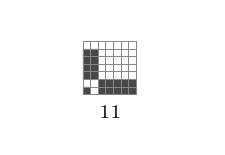
\begin{tikzpicture}[x=1mm,y=1mm,baseline=0mm]
\path[use as bounding box] (0,-.7) rectangle (21.5,11.9);
\begin{scope}[shift={(7.0,3.4)},x=0.97mm,y=0.97mm]
\fill[black!72] (0,5) rectangle (1,6) (1,5) rectangle (2,6) (0,4) rectangle (1,5) (1,4) rectangle (2,5) (0,3) rectangle (1,4) (1,3) rectangle (2,4) (0,2) rectangle (1,3) (1,2) rectangle (2,3) (2,1) rectangle (3,2) (3,1) rectangle (4,2) (4,1) rectangle (5,2) (5,1) rectangle (6,2) (6,1) rectangle (7,2) (0,0) rectangle (1,1) (2,0) rectangle (3,1) (3,0) rectangle (4,1) (4,0) rectangle (5,1) (5,0) rectangle (6,1) (6,0) rectangle (7,1);
\draw[black!47,line width=.16pt] (0,0)--(0,7) (0,0)--(7,0) (1,0)--(1,7) (0,1)--(7,1) (2,0)--(2,7) (0,2)--(7,2) (3,0)--(3,7) (0,3)--(7,3) (4,0)--(4,7) (0,4)--(7,4) (5,0)--(5,7) (0,5)--(7,5) (6,0)--(6,7) (0,6)--(7,6) (7,0)--(7,7) (0,7)--(7,7);
\end{scope}
\node[inner sep=0pt,font=\scriptsize] at (10.5,1.1) {$11$};
\end{tikzpicture} &
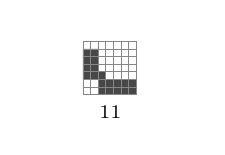
\begin{tikzpicture}[x=1mm,y=1mm,baseline=0mm]
\path[use as bounding box] (0,-.7) rectangle (21.5,11.9);
\begin{scope}[shift={(7.0,3.4)},x=0.97mm,y=0.97mm]
\fill[black!72] (0,5) rectangle (1,6) (1,5) rectangle (2,6) (0,4) rectangle (1,5) (1,4) rectangle (2,5) (0,3) rectangle (1,4) (1,3) rectangle (2,4) (0,2) rectangle (1,3) (1,2) rectangle (2,3) (2,2) rectangle (3,3) (2,1) rectangle (3,2) (3,1) rectangle (4,2) (4,1) rectangle (5,2) (5,1) rectangle (6,2) (6,1) rectangle (7,2) (2,0) rectangle (3,1) (3,0) rectangle (4,1) (4,0) rectangle (5,1) (5,0) rectangle (6,1) (6,0) rectangle (7,1);
\draw[black!47,line width=.16pt] (0,0)--(0,7) (0,0)--(7,0) (1,0)--(1,7) (0,1)--(7,1) (2,0)--(2,7) (0,2)--(7,2) (3,0)--(3,7) (0,3)--(7,3) (4,0)--(4,7) (0,4)--(7,4) (5,0)--(5,7) (0,5)--(7,5) (6,0)--(6,7) (0,6)--(7,6) (7,0)--(7,7) (0,7)--(7,7);
\end{scope}
\node[inner sep=0pt,font=\scriptsize] at (10.5,1.1) {$11$};
\end{tikzpicture} &
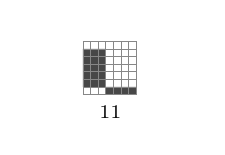
\begin{tikzpicture}[x=1mm,y=1mm,baseline=0mm]
\path[use as bounding box] (0,-.7) rectangle (21.5,11.9);
\begin{scope}[shift={(7.0,3.4)},x=0.97mm,y=0.97mm]
\fill[black!72] (0,5) rectangle (1,6) (1,5) rectangle (2,6) (2,5) rectangle (3,6) (0,4) rectangle (1,5) (1,4) rectangle (2,5) (2,4) rectangle (3,5) (0,3) rectangle (1,4) (1,3) rectangle (2,4) (2,3) rectangle (3,4) (0,2) rectangle (1,3) (1,2) rectangle (2,3) (2,2) rectangle (3,3) (0,1) rectangle (1,2) (1,1) rectangle (2,2) (2,1) rectangle (3,2) (3,0) rectangle (4,1) (4,0) rectangle (5,1) (5,0) rectangle (6,1) (6,0) rectangle (7,1);
\draw[black!47,line width=.16pt] (0,0)--(0,7) (0,0)--(7,0) (1,0)--(1,7) (0,1)--(7,1) (2,0)--(2,7) (0,2)--(7,2) (3,0)--(3,7) (0,3)--(7,3) (4,0)--(4,7) (0,4)--(7,4) (5,0)--(5,7) (0,5)--(7,5) (6,0)--(6,7) (0,6)--(7,6) (7,0)--(7,7) (0,7)--(7,7);
\end{scope}
\node[inner sep=0pt,font=\scriptsize] at (10.5,1.1) {$11$};
\end{tikzpicture} &
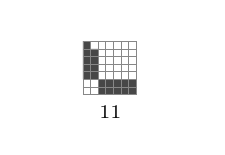
\begin{tikzpicture}[x=1mm,y=1mm,baseline=0mm]
\path[use as bounding box] (0,-.7) rectangle (21.5,11.9);
\begin{scope}[shift={(7.0,3.4)},x=0.97mm,y=0.97mm]
\fill[black!72] (0,6) rectangle (1,7) (0,5) rectangle (1,6) (1,5) rectangle (2,6) (0,4) rectangle (1,5) (1,4) rectangle (2,5) (0,3) rectangle (1,4) (1,3) rectangle (2,4) (0,2) rectangle (1,3) (1,2) rectangle (2,3) (2,1) rectangle (3,2) (3,1) rectangle (4,2) (4,1) rectangle (5,2) (5,1) rectangle (6,2) (6,1) rectangle (7,2) (2,0) rectangle (3,1) (3,0) rectangle (4,1) (4,0) rectangle (5,1) (5,0) rectangle (6,1) (6,0) rectangle (7,1);
\draw[black!47,line width=.16pt] (0,0)--(0,7) (0,0)--(7,0) (1,0)--(1,7) (0,1)--(7,1) (2,0)--(2,7) (0,2)--(7,2) (3,0)--(3,7) (0,3)--(7,3) (4,0)--(4,7) (0,4)--(7,4) (5,0)--(5,7) (0,5)--(7,5) (6,0)--(6,7) (0,6)--(7,6) (7,0)--(7,7) (0,7)--(7,7);
\end{scope}
\node[inner sep=0pt,font=\scriptsize] at (10.5,1.1) {$11$};
\end{tikzpicture} &
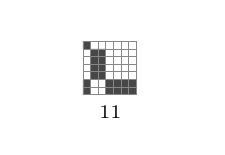
\begin{tikzpicture}[x=1mm,y=1mm,baseline=0mm]
\path[use as bounding box] (0,-.7) rectangle (21.5,11.9);
\begin{scope}[shift={(7.0,3.4)},x=0.97mm,y=0.97mm]
\fill[black!72] (0,6) rectangle (1,7) (1,5) rectangle (2,6) (2,5) rectangle (3,6) (1,4) rectangle (2,5) (2,4) rectangle (3,5) (1,3) rectangle (2,4) (2,3) rectangle (3,4) (1,2) rectangle (2,3) (2,2) rectangle (3,3) (0,1) rectangle (1,2) (3,1) rectangle (4,2) (4,1) rectangle (5,2) (5,1) rectangle (6,2) (6,1) rectangle (7,2) (0,0) rectangle (1,1) (3,0) rectangle (4,1) (4,0) rectangle (5,1) (5,0) rectangle (6,1) (6,0) rectangle (7,1);
\draw[black!47,line width=.16pt] (0,0)--(0,7) (0,0)--(7,0) (1,0)--(1,7) (0,1)--(7,1) (2,0)--(2,7) (0,2)--(7,2) (3,0)--(3,7) (0,3)--(7,3) (4,0)--(4,7) (0,4)--(7,4) (5,0)--(5,7) (0,5)--(7,5) (6,0)--(6,7) (0,6)--(7,6) (7,0)--(7,7) (0,7)--(7,7);
\end{scope}
\node[inner sep=0pt,font=\scriptsize] at (10.5,1.1) {$11$};
\end{tikzpicture} \\[.4mm]
\end{tabular}
\caption{Cross adjacencies tested in the connected case, part 1 of 2.}
\label{fig:nine-qfourteen-connected}
\end{figure}

\begin{figure}[!htbp]
\centering
\begin{tabular}{@{}c@{\hspace{1.6mm}}c@{\hspace{1.6mm}}c@{\hspace{1.6mm}}c@{\hspace{1.6mm}}c@{}}
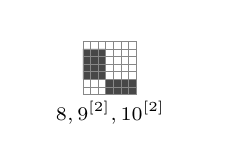
\begin{tikzpicture}[x=1mm,y=1mm,baseline=0mm]
\path[use as bounding box] (0,-.7) rectangle (21.5,11.9);
\begin{scope}[shift={(7.0,3.4)},x=0.97mm,y=0.97mm]
\fill[black!72] (0,5) rectangle (1,6) (1,5) rectangle (2,6) (2,5) rectangle (3,6) (0,4) rectangle (1,5) (1,4) rectangle (2,5) (2,4) rectangle (3,5) (0,3) rectangle (1,4) (1,3) rectangle (2,4) (2,3) rectangle (3,4) (0,2) rectangle (1,3) (1,2) rectangle (2,3) (2,2) rectangle (3,3) (3,1) rectangle (4,2) (4,1) rectangle (5,2) (5,1) rectangle (6,2) (6,1) rectangle (7,2) (3,0) rectangle (4,1) (4,0) rectangle (5,1) (5,0) rectangle (6,1) (6,0) rectangle (7,1);
\draw[black!47,line width=.16pt] (0,0)--(0,7) (0,0)--(7,0) (1,0)--(1,7) (0,1)--(7,1) (2,0)--(2,7) (0,2)--(7,2) (3,0)--(3,7) (0,3)--(7,3) (4,0)--(4,7) (0,4)--(7,4) (5,0)--(5,7) (0,5)--(7,5) (6,0)--(6,7) (0,6)--(7,6) (7,0)--(7,7) (0,7)--(7,7);
\end{scope}
\node[inner sep=0pt,font=\scriptsize] at (10.5,1.1) {$8,9^{[2]},10^{[2]}$};
\end{tikzpicture} &
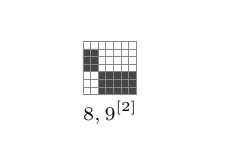
\begin{tikzpicture}[x=1mm,y=1mm,baseline=0mm]
\path[use as bounding box] (0,-.7) rectangle (21.5,11.9);
\begin{scope}[shift={(7.0,3.4)},x=0.97mm,y=0.97mm]
\fill[black!72] (0,5) rectangle (1,6) (1,5) rectangle (2,6) (0,4) rectangle (1,5) (1,4) rectangle (2,5) (0,3) rectangle (1,4) (1,3) rectangle (2,4) (2,2) rectangle (3,3) (3,2) rectangle (4,3) (4,2) rectangle (5,3) (5,2) rectangle (6,3) (6,2) rectangle (7,3) (2,1) rectangle (3,2) (3,1) rectangle (4,2) (4,1) rectangle (5,2) (5,1) rectangle (6,2) (6,1) rectangle (7,2) (2,0) rectangle (3,1) (3,0) rectangle (4,1) (4,0) rectangle (5,1) (5,0) rectangle (6,1) (6,0) rectangle (7,1);
\draw[black!47,line width=.16pt] (0,0)--(0,7) (0,0)--(7,0) (1,0)--(1,7) (0,1)--(7,1) (2,0)--(2,7) (0,2)--(7,2) (3,0)--(3,7) (0,3)--(7,3) (4,0)--(4,7) (0,4)--(7,4) (5,0)--(5,7) (0,5)--(7,5) (6,0)--(6,7) (0,6)--(7,6) (7,0)--(7,7) (0,7)--(7,7);
\end{scope}
\node[inner sep=0pt,font=\scriptsize] at (10.5,1.1) {$8,9^{[2]}$};
\end{tikzpicture} &
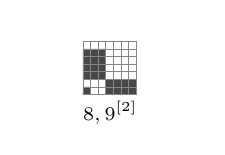
\begin{tikzpicture}[x=1mm,y=1mm,baseline=0mm]
\path[use as bounding box] (0,-.7) rectangle (21.5,11.9);
\begin{scope}[shift={(7.0,3.4)},x=0.97mm,y=0.97mm]
\fill[black!72] (0,5) rectangle (1,6) (1,5) rectangle (2,6) (2,5) rectangle (3,6) (0,4) rectangle (1,5) (1,4) rectangle (2,5) (2,4) rectangle (3,5) (0,3) rectangle (1,4) (1,3) rectangle (2,4) (2,3) rectangle (3,4) (0,2) rectangle (1,3) (1,2) rectangle (2,3) (2,2) rectangle (3,3) (3,1) rectangle (4,2) (4,1) rectangle (5,2) (5,1) rectangle (6,2) (6,1) rectangle (7,2) (0,0) rectangle (1,1) (3,0) rectangle (4,1) (4,0) rectangle (5,1) (5,0) rectangle (6,1) (6,0) rectangle (7,1);
\draw[black!47,line width=.16pt] (0,0)--(0,7) (0,0)--(7,0) (1,0)--(1,7) (0,1)--(7,1) (2,0)--(2,7) (0,2)--(7,2) (3,0)--(3,7) (0,3)--(7,3) (4,0)--(4,7) (0,4)--(7,4) (5,0)--(5,7) (0,5)--(7,5) (6,0)--(6,7) (0,6)--(7,6) (7,0)--(7,7) (0,7)--(7,7);
\end{scope}
\node[inner sep=0pt,font=\scriptsize] at (10.5,1.1) {$8,9^{[2]}$};
\end{tikzpicture} &
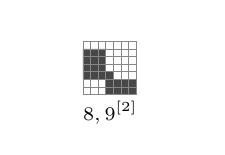
\begin{tikzpicture}[x=1mm,y=1mm,baseline=0mm]
\path[use as bounding box] (0,-.7) rectangle (21.5,11.9);
\begin{scope}[shift={(7.0,3.4)},x=0.97mm,y=0.97mm]
\fill[black!72] (0,5) rectangle (1,6) (1,5) rectangle (2,6) (2,5) rectangle (3,6) (0,4) rectangle (1,5) (1,4) rectangle (2,5) (2,4) rectangle (3,5) (0,3) rectangle (1,4) (1,3) rectangle (2,4) (2,3) rectangle (3,4) (0,2) rectangle (1,3) (1,2) rectangle (2,3) (2,2) rectangle (3,3) (3,2) rectangle (4,3) (3,1) rectangle (4,2) (4,1) rectangle (5,2) (5,1) rectangle (6,2) (6,1) rectangle (7,2) (3,0) rectangle (4,1) (4,0) rectangle (5,1) (5,0) rectangle (6,1) (6,0) rectangle (7,1);
\draw[black!47,line width=.16pt] (0,0)--(0,7) (0,0)--(7,0) (1,0)--(1,7) (0,1)--(7,1) (2,0)--(2,7) (0,2)--(7,2) (3,0)--(3,7) (0,3)--(7,3) (4,0)--(4,7) (0,4)--(7,4) (5,0)--(5,7) (0,5)--(7,5) (6,0)--(6,7) (0,6)--(7,6) (7,0)--(7,7) (0,7)--(7,7);
\end{scope}
\node[inner sep=0pt,font=\scriptsize] at (10.5,1.1) {$8,9^{[2]}$};
\end{tikzpicture} &
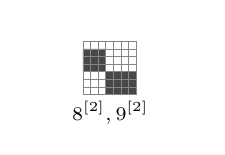
\begin{tikzpicture}[x=1mm,y=1mm,baseline=0mm]
\path[use as bounding box] (0,-.7) rectangle (21.5,11.9);
\begin{scope}[shift={(7.0,3.4)},x=0.97mm,y=0.97mm]
\fill[black!72] (0,5) rectangle (1,6) (1,5) rectangle (2,6) (2,5) rectangle (3,6) (0,4) rectangle (1,5) (1,4) rectangle (2,5) (2,4) rectangle (3,5) (0,3) rectangle (1,4) (1,3) rectangle (2,4) (2,3) rectangle (3,4) (3,2) rectangle (4,3) (4,2) rectangle (5,3) (5,2) rectangle (6,3) (6,2) rectangle (7,3) (3,1) rectangle (4,2) (4,1) rectangle (5,2) (5,1) rectangle (6,2) (6,1) rectangle (7,2) (3,0) rectangle (4,1) (4,0) rectangle (5,1) (5,0) rectangle (6,1) (6,0) rectangle (7,1);
\draw[black!47,line width=.16pt] (0,0)--(0,7) (0,0)--(7,0) (1,0)--(1,7) (0,1)--(7,1) (2,0)--(2,7) (0,2)--(7,2) (3,0)--(3,7) (0,3)--(7,3) (4,0)--(4,7) (0,4)--(7,4) (5,0)--(5,7) (0,5)--(7,5) (6,0)--(6,7) (0,6)--(7,6) (7,0)--(7,7) (0,7)--(7,7);
\end{scope}
\node[inner sep=0pt,font=\scriptsize] at (10.5,1.1) {$8^{[2]},9^{[2]}$};
\end{tikzpicture} \\[.4mm]
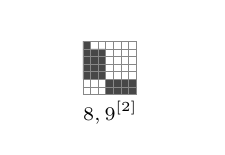
\begin{tikzpicture}[x=1mm,y=1mm,baseline=0mm]
\path[use as bounding box] (0,-.7) rectangle (21.5,11.9);
\begin{scope}[shift={(7.0,3.4)},x=0.97mm,y=0.97mm]
\fill[black!72] (0,6) rectangle (1,7) (0,5) rectangle (1,6) (1,5) rectangle (2,6) (2,5) rectangle (3,6) (0,4) rectangle (1,5) (1,4) rectangle (2,5) (2,4) rectangle (3,5) (0,3) rectangle (1,4) (1,3) rectangle (2,4) (2,3) rectangle (3,4) (0,2) rectangle (1,3) (1,2) rectangle (2,3) (2,2) rectangle (3,3) (3,1) rectangle (4,2) (4,1) rectangle (5,2) (5,1) rectangle (6,2) (6,1) rectangle (7,2) (3,0) rectangle (4,1) (4,0) rectangle (5,1) (5,0) rectangle (6,1) (6,0) rectangle (7,1);
\draw[black!47,line width=.16pt] (0,0)--(0,7) (0,0)--(7,0) (1,0)--(1,7) (0,1)--(7,1) (2,0)--(2,7) (0,2)--(7,2) (3,0)--(3,7) (0,3)--(7,3) (4,0)--(4,7) (0,4)--(7,4) (5,0)--(5,7) (0,5)--(7,5) (6,0)--(6,7) (0,6)--(7,6) (7,0)--(7,7) (0,7)--(7,7);
\end{scope}
\node[inner sep=0pt,font=\scriptsize] at (10.5,1.1) {$8,9^{[2]}$};
\end{tikzpicture} &
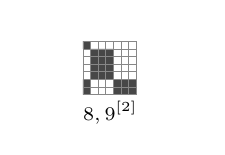
\begin{tikzpicture}[x=1mm,y=1mm,baseline=0mm]
\path[use as bounding box] (0,-.7) rectangle (21.5,11.9);
\begin{scope}[shift={(7.0,3.4)},x=0.97mm,y=0.97mm]
\fill[black!72] (0,6) rectangle (1,7) (1,5) rectangle (2,6) (2,5) rectangle (3,6) (3,5) rectangle (4,6) (1,4) rectangle (2,5) (2,4) rectangle (3,5) (3,4) rectangle (4,5) (1,3) rectangle (2,4) (2,3) rectangle (3,4) (3,3) rectangle (4,4) (1,2) rectangle (2,3) (2,2) rectangle (3,3) (3,2) rectangle (4,3) (0,1) rectangle (1,2) (4,1) rectangle (5,2) (5,1) rectangle (6,2) (6,1) rectangle (7,2) (0,0) rectangle (1,1) (4,0) rectangle (5,1) (5,0) rectangle (6,1) (6,0) rectangle (7,1);
\draw[black!47,line width=.16pt] (0,0)--(0,7) (0,0)--(7,0) (1,0)--(1,7) (0,1)--(7,1) (2,0)--(2,7) (0,2)--(7,2) (3,0)--(3,7) (0,3)--(7,3) (4,0)--(4,7) (0,4)--(7,4) (5,0)--(5,7) (0,5)--(7,5) (6,0)--(6,7) (0,6)--(7,6) (7,0)--(7,7) (0,7)--(7,7);
\end{scope}
\node[inner sep=0pt,font=\scriptsize] at (10.5,1.1) {$8,9^{[2]}$};
\end{tikzpicture} &
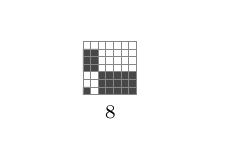
\begin{tikzpicture}[x=1mm,y=1mm,baseline=0mm]
\path[use as bounding box] (0,-.7) rectangle (21.5,11.9);
\begin{scope}[shift={(7.0,3.4)},x=0.97mm,y=0.97mm]
\fill[black!72] (0,5) rectangle (1,6) (1,5) rectangle (2,6) (0,4) rectangle (1,5) (1,4) rectangle (2,5) (0,3) rectangle (1,4) (1,3) rectangle (2,4) (2,2) rectangle (3,3) (3,2) rectangle (4,3) (4,2) rectangle (5,3) (5,2) rectangle (6,3) (6,2) rectangle (7,3) (2,1) rectangle (3,2) (3,1) rectangle (4,2) (4,1) rectangle (5,2) (5,1) rectangle (6,2) (6,1) rectangle (7,2) (0,0) rectangle (1,1) (2,0) rectangle (3,1) (3,0) rectangle (4,1) (4,0) rectangle (5,1) (5,0) rectangle (6,1) (6,0) rectangle (7,1);
\draw[black!47,line width=.16pt] (0,0)--(0,7) (0,0)--(7,0) (1,0)--(1,7) (0,1)--(7,1) (2,0)--(2,7) (0,2)--(7,2) (3,0)--(3,7) (0,3)--(7,3) (4,0)--(4,7) (0,4)--(7,4) (5,0)--(5,7) (0,5)--(7,5) (6,0)--(6,7) (0,6)--(7,6) (7,0)--(7,7) (0,7)--(7,7);
\end{scope}
\node[inner sep=0pt,font=\scriptsize] at (10.5,1.1) {$8$};
\end{tikzpicture} &
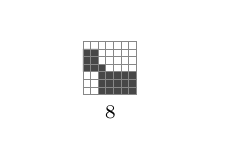
\begin{tikzpicture}[x=1mm,y=1mm,baseline=0mm]
\path[use as bounding box] (0,-.7) rectangle (21.5,11.9);
\begin{scope}[shift={(7.0,3.4)},x=0.97mm,y=0.97mm]
\fill[black!72] (0,5) rectangle (1,6) (1,5) rectangle (2,6) (0,4) rectangle (1,5) (1,4) rectangle (2,5) (0,3) rectangle (1,4) (1,3) rectangle (2,4) (2,3) rectangle (3,4) (2,2) rectangle (3,3) (3,2) rectangle (4,3) (4,2) rectangle (5,3) (5,2) rectangle (6,3) (6,2) rectangle (7,3) (2,1) rectangle (3,2) (3,1) rectangle (4,2) (4,1) rectangle (5,2) (5,1) rectangle (6,2) (6,1) rectangle (7,2) (2,0) rectangle (3,1) (3,0) rectangle (4,1) (4,0) rectangle (5,1) (5,0) rectangle (6,1) (6,0) rectangle (7,1);
\draw[black!47,line width=.16pt] (0,0)--(0,7) (0,0)--(7,0) (1,0)--(1,7) (0,1)--(7,1) (2,0)--(2,7) (0,2)--(7,2) (3,0)--(3,7) (0,3)--(7,3) (4,0)--(4,7) (0,4)--(7,4) (5,0)--(5,7) (0,5)--(7,5) (6,0)--(6,7) (0,6)--(7,6) (7,0)--(7,7) (0,7)--(7,7);
\end{scope}
\node[inner sep=0pt,font=\scriptsize] at (10.5,1.1) {$8$};
\end{tikzpicture} &
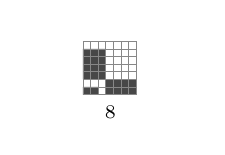
\begin{tikzpicture}[x=1mm,y=1mm,baseline=0mm]
\path[use as bounding box] (0,-.7) rectangle (21.5,11.9);
\begin{scope}[shift={(7.0,3.4)},x=0.97mm,y=0.97mm]
\fill[black!72] (0,5) rectangle (1,6) (1,5) rectangle (2,6) (2,5) rectangle (3,6) (0,4) rectangle (1,5) (1,4) rectangle (2,5) (2,4) rectangle (3,5) (0,3) rectangle (1,4) (1,3) rectangle (2,4) (2,3) rectangle (3,4) (0,2) rectangle (1,3) (1,2) rectangle (2,3) (2,2) rectangle (3,3) (3,1) rectangle (4,2) (4,1) rectangle (5,2) (5,1) rectangle (6,2) (6,1) rectangle (7,2) (0,0) rectangle (1,1) (1,0) rectangle (2,1) (3,0) rectangle (4,1) (4,0) rectangle (5,1) (5,0) rectangle (6,1) (6,0) rectangle (7,1);
\draw[black!47,line width=.16pt] (0,0)--(0,7) (0,0)--(7,0) (1,0)--(1,7) (0,1)--(7,1) (2,0)--(2,7) (0,2)--(7,2) (3,0)--(3,7) (0,3)--(7,3) (4,0)--(4,7) (0,4)--(7,4) (5,0)--(5,7) (0,5)--(7,5) (6,0)--(6,7) (0,6)--(7,6) (7,0)--(7,7) (0,7)--(7,7);
\end{scope}
\node[inner sep=0pt,font=\scriptsize] at (10.5,1.1) {$8$};
\end{tikzpicture} \\[.4mm]
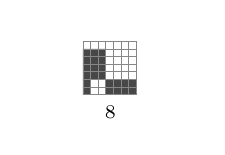
\begin{tikzpicture}[x=1mm,y=1mm,baseline=0mm]
\path[use as bounding box] (0,-.7) rectangle (21.5,11.9);
\begin{scope}[shift={(7.0,3.4)},x=0.97mm,y=0.97mm]
\fill[black!72] (0,5) rectangle (1,6) (1,5) rectangle (2,6) (2,5) rectangle (3,6) (0,4) rectangle (1,5) (1,4) rectangle (2,5) (2,4) rectangle (3,5) (0,3) rectangle (1,4) (1,3) rectangle (2,4) (2,3) rectangle (3,4) (0,2) rectangle (1,3) (1,2) rectangle (2,3) (2,2) rectangle (3,3) (0,1) rectangle (1,2) (3,1) rectangle (4,2) (4,1) rectangle (5,2) (5,1) rectangle (6,2) (6,1) rectangle (7,2) (0,0) rectangle (1,1) (3,0) rectangle (4,1) (4,0) rectangle (5,1) (5,0) rectangle (6,1) (6,0) rectangle (7,1);
\draw[black!47,line width=.16pt] (0,0)--(0,7) (0,0)--(7,0) (1,0)--(1,7) (0,1)--(7,1) (2,0)--(2,7) (0,2)--(7,2) (3,0)--(3,7) (0,3)--(7,3) (4,0)--(4,7) (0,4)--(7,4) (5,0)--(5,7) (0,5)--(7,5) (6,0)--(6,7) (0,6)--(7,6) (7,0)--(7,7) (0,7)--(7,7);
\end{scope}
\node[inner sep=0pt,font=\scriptsize] at (10.5,1.1) {$8$};
\end{tikzpicture} &
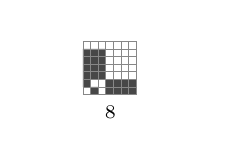
\begin{tikzpicture}[x=1mm,y=1mm,baseline=0mm]
\path[use as bounding box] (0,-.7) rectangle (21.5,11.9);
\begin{scope}[shift={(7.0,3.4)},x=0.97mm,y=0.97mm]
\fill[black!72] (0,5) rectangle (1,6) (1,5) rectangle (2,6) (2,5) rectangle (3,6) (0,4) rectangle (1,5) (1,4) rectangle (2,5) (2,4) rectangle (3,5) (0,3) rectangle (1,4) (1,3) rectangle (2,4) (2,3) rectangle (3,4) (0,2) rectangle (1,3) (1,2) rectangle (2,3) (2,2) rectangle (3,3) (0,1) rectangle (1,2) (3,1) rectangle (4,2) (4,1) rectangle (5,2) (5,1) rectangle (6,2) (6,1) rectangle (7,2) (1,0) rectangle (2,1) (3,0) rectangle (4,1) (4,0) rectangle (5,1) (5,0) rectangle (6,1) (6,0) rectangle (7,1);
\draw[black!47,line width=.16pt] (0,0)--(0,7) (0,0)--(7,0) (1,0)--(1,7) (0,1)--(7,1) (2,0)--(2,7) (0,2)--(7,2) (3,0)--(3,7) (0,3)--(7,3) (4,0)--(4,7) (0,4)--(7,4) (5,0)--(5,7) (0,5)--(7,5) (6,0)--(6,7) (0,6)--(7,6) (7,0)--(7,7) (0,7)--(7,7);
\end{scope}
\node[inner sep=0pt,font=\scriptsize] at (10.5,1.1) {$8$};
\end{tikzpicture} &
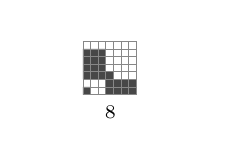
\begin{tikzpicture}[x=1mm,y=1mm,baseline=0mm]
\path[use as bounding box] (0,-.7) rectangle (21.5,11.9);
\begin{scope}[shift={(7.0,3.4)},x=0.97mm,y=0.97mm]
\fill[black!72] (0,5) rectangle (1,6) (1,5) rectangle (2,6) (2,5) rectangle (3,6) (0,4) rectangle (1,5) (1,4) rectangle (2,5) (2,4) rectangle (3,5) (0,3) rectangle (1,4) (1,3) rectangle (2,4) (2,3) rectangle (3,4) (0,2) rectangle (1,3) (1,2) rectangle (2,3) (2,2) rectangle (3,3) (3,2) rectangle (4,3) (3,1) rectangle (4,2) (4,1) rectangle (5,2) (5,1) rectangle (6,2) (6,1) rectangle (7,2) (0,0) rectangle (1,1) (3,0) rectangle (4,1) (4,0) rectangle (5,1) (5,0) rectangle (6,1) (6,0) rectangle (7,1);
\draw[black!47,line width=.16pt] (0,0)--(0,7) (0,0)--(7,0) (1,0)--(1,7) (0,1)--(7,1) (2,0)--(2,7) (0,2)--(7,2) (3,0)--(3,7) (0,3)--(7,3) (4,0)--(4,7) (0,4)--(7,4) (5,0)--(5,7) (0,5)--(7,5) (6,0)--(6,7) (0,6)--(7,6) (7,0)--(7,7) (0,7)--(7,7);
\end{scope}
\node[inner sep=0pt,font=\scriptsize] at (10.5,1.1) {$8$};
\end{tikzpicture} &
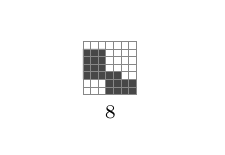
\begin{tikzpicture}[x=1mm,y=1mm,baseline=0mm]
\path[use as bounding box] (0,-.7) rectangle (21.5,11.9);
\begin{scope}[shift={(7.0,3.4)},x=0.97mm,y=0.97mm]
\fill[black!72] (0,5) rectangle (1,6) (1,5) rectangle (2,6) (2,5) rectangle (3,6) (0,4) rectangle (1,5) (1,4) rectangle (2,5) (2,4) rectangle (3,5) (0,3) rectangle (1,4) (1,3) rectangle (2,4) (2,3) rectangle (3,4) (0,2) rectangle (1,3) (1,2) rectangle (2,3) (2,2) rectangle (3,3) (3,2) rectangle (4,3) (4,2) rectangle (5,3) (3,1) rectangle (4,2) (4,1) rectangle (5,2) (5,1) rectangle (6,2) (6,1) rectangle (7,2) (3,0) rectangle (4,1) (4,0) rectangle (5,1) (5,0) rectangle (6,1) (6,0) rectangle (7,1);
\draw[black!47,line width=.16pt] (0,0)--(0,7) (0,0)--(7,0) (1,0)--(1,7) (0,1)--(7,1) (2,0)--(2,7) (0,2)--(7,2) (3,0)--(3,7) (0,3)--(7,3) (4,0)--(4,7) (0,4)--(7,4) (5,0)--(5,7) (0,5)--(7,5) (6,0)--(6,7) (0,6)--(7,6) (7,0)--(7,7) (0,7)--(7,7);
\end{scope}
\node[inner sep=0pt,font=\scriptsize] at (10.5,1.1) {$8$};
\end{tikzpicture} &
\begin{tikzpicture}[x=1mm,y=1mm,baseline=0mm]
\path[use as bounding box] (0,-.7) rectangle (21.5,11.9);
\begin{scope}[shift={(7.0,3.4)},x=0.97mm,y=0.97mm]
\fill[black!72] (0,5) rectangle (1,6) (1,5) rectangle (2,6) (2,5) rectangle (3,6) (0,4) rectangle (1,5) (1,4) rectangle (2,5) (2,4) rectangle (3,5) (0,3) rectangle (1,4) (1,3) rectangle (2,4) (2,3) rectangle (3,4) (3,2) rectangle (4,3) (4,2) rectangle (5,3) (5,2) rectangle (6,3) (6,2) rectangle (7,3) (3,1) rectangle (4,2) (4,1) rectangle (5,2) (5,1) rectangle (6,2) (6,1) rectangle (7,2) (0,0) rectangle (1,1) (3,0) rectangle (4,1) (4,0) rectangle (5,1) (5,0) rectangle (6,1) (6,0) rectangle (7,1);
\draw[black!47,line width=.16pt] (0,0)--(0,7) (0,0)--(7,0) (1,0)--(1,7) (0,1)--(7,1) (2,0)--(2,7) (0,2)--(7,2) (3,0)--(3,7) (0,3)--(7,3) (4,0)--(4,7) (0,4)--(7,4) (5,0)--(5,7) (0,5)--(7,5) (6,0)--(6,7) (0,6)--(7,6) (7,0)--(7,7) (0,7)--(7,7);
\end{scope}
\node[inner sep=0pt,font=\scriptsize] at (10.5,1.1) {$8^{[2]}$};
\end{tikzpicture} \\[.4mm]
\begin{tikzpicture}[x=1mm,y=1mm,baseline=0mm]
\path[use as bounding box] (0,-.7) rectangle (21.5,11.9);
\begin{scope}[shift={(7.0,3.4)},x=0.97mm,y=0.97mm]
\fill[black!72] (0,5) rectangle (1,6) (1,5) rectangle (2,6) (2,5) rectangle (3,6) (0,4) rectangle (1,5) (1,4) rectangle (2,5) (2,4) rectangle (3,5) (0,3) rectangle (1,4) (1,3) rectangle (2,4) (2,3) rectangle (3,4) (3,3) rectangle (4,4) (0,2) rectangle (1,3) (1,2) rectangle (2,3) (2,2) rectangle (3,3) (3,2) rectangle (4,3) (3,1) rectangle (4,2) (4,1) rectangle (5,2) (5,1) rectangle (6,2) (6,1) rectangle (7,2) (3,0) rectangle (4,1) (4,0) rectangle (5,1) (5,0) rectangle (6,1) (6,0) rectangle (7,1);
\draw[black!47,line width=.16pt] (0,0)--(0,7) (0,0)--(7,0) (1,0)--(1,7) (0,1)--(7,1) (2,0)--(2,7) (0,2)--(7,2) (3,0)--(3,7) (0,3)--(7,3) (4,0)--(4,7) (0,4)--(7,4) (5,0)--(5,7) (0,5)--(7,5) (6,0)--(6,7) (0,6)--(7,6) (7,0)--(7,7) (0,7)--(7,7);
\end{scope}
\node[inner sep=0pt,font=\scriptsize] at (10.5,1.1) {$8$};
\end{tikzpicture} &
\begin{tikzpicture}[x=1mm,y=1mm,baseline=0mm]
\path[use as bounding box] (0,-.7) rectangle (21.5,11.9);
\begin{scope}[shift={(7.0,3.4)},x=0.97mm,y=0.97mm]
\fill[black!72] (0,5) rectangle (1,6) (1,5) rectangle (2,6) (2,5) rectangle (3,6) (0,4) rectangle (1,5) (1,4) rectangle (2,5) (2,4) rectangle (3,5) (0,3) rectangle (1,4) (1,3) rectangle (2,4) (2,3) rectangle (3,4) (3,3) rectangle (4,4) (0,2) rectangle (1,3) (1,2) rectangle (2,3) (2,2) rectangle (3,3) (4,2) rectangle (5,3) (3,1) rectangle (4,2) (4,1) rectangle (5,2) (5,1) rectangle (6,2) (6,1) rectangle (7,2) (3,0) rectangle (4,1) (4,0) rectangle (5,1) (5,0) rectangle (6,1) (6,0) rectangle (7,1);
\draw[black!47,line width=.16pt] (0,0)--(0,7) (0,0)--(7,0) (1,0)--(1,7) (0,1)--(7,1) (2,0)--(2,7) (0,2)--(7,2) (3,0)--(3,7) (0,3)--(7,3) (4,0)--(4,7) (0,4)--(7,4) (5,0)--(5,7) (0,5)--(7,5) (6,0)--(6,7) (0,6)--(7,6) (7,0)--(7,7) (0,7)--(7,7);
\end{scope}
\node[inner sep=0pt,font=\scriptsize] at (10.5,1.1) {$8$};
\end{tikzpicture} &
\begin{tikzpicture}[x=1mm,y=1mm,baseline=0mm]
\path[use as bounding box] (0,-.7) rectangle (21.5,11.9);
\begin{scope}[shift={(7.0,3.4)},x=0.97mm,y=0.97mm]
\fill[black!72] (0,5) rectangle (1,6) (1,5) rectangle (2,6) (2,5) rectangle (3,6) (0,4) rectangle (1,5) (1,4) rectangle (2,5) (2,4) rectangle (3,5) (0,3) rectangle (1,4) (1,3) rectangle (2,4) (2,3) rectangle (3,4) (3,3) rectangle (4,4) (3,2) rectangle (4,3) (4,2) rectangle (5,3) (5,2) rectangle (6,3) (6,2) rectangle (7,3) (3,1) rectangle (4,2) (4,1) rectangle (5,2) (5,1) rectangle (6,2) (6,1) rectangle (7,2) (3,0) rectangle (4,1) (4,0) rectangle (5,1) (5,0) rectangle (6,1) (6,0) rectangle (7,1);
\draw[black!47,line width=.16pt] (0,0)--(0,7) (0,0)--(7,0) (1,0)--(1,7) (0,1)--(7,1) (2,0)--(2,7) (0,2)--(7,2) (3,0)--(3,7) (0,3)--(7,3) (4,0)--(4,7) (0,4)--(7,4) (5,0)--(5,7) (0,5)--(7,5) (6,0)--(6,7) (0,6)--(7,6) (7,0)--(7,7) (0,7)--(7,7);
\end{scope}
\node[inner sep=0pt,font=\scriptsize] at (10.5,1.1) {$8^{[2]}$};
\end{tikzpicture} &
\begin{tikzpicture}[x=1mm,y=1mm,baseline=0mm]
\path[use as bounding box] (0,-.7) rectangle (21.5,11.9);
\begin{scope}[shift={(7.0,3.4)},x=0.97mm,y=0.97mm]
\fill[black!72] (0,5) rectangle (1,6) (1,5) rectangle (2,6) (2,5) rectangle (3,6) (0,4) rectangle (1,5) (1,4) rectangle (2,5) (2,4) rectangle (3,5) (3,3) rectangle (4,4) (4,3) rectangle (5,4) (5,3) rectangle (6,4) (6,3) rectangle (7,4) (3,2) rectangle (4,3) (4,2) rectangle (5,3) (5,2) rectangle (6,3) (6,2) rectangle (7,3) (3,1) rectangle (4,2) (4,1) rectangle (5,2) (5,1) rectangle (6,2) (6,1) rectangle (7,2) (3,0) rectangle (4,1) (4,0) rectangle (5,1) (5,0) rectangle (6,1) (6,0) rectangle (7,1);
\draw[black!47,line width=.16pt] (0,0)--(0,7) (0,0)--(7,0) (1,0)--(1,7) (0,1)--(7,1) (2,0)--(2,7) (0,2)--(7,2) (3,0)--(3,7) (0,3)--(7,3) (4,0)--(4,7) (0,4)--(7,4) (5,0)--(5,7) (0,5)--(7,5) (6,0)--(6,7) (0,6)--(7,6) (7,0)--(7,7) (0,7)--(7,7);
\end{scope}
\node[inner sep=0pt,font=\scriptsize] at (10.5,1.1) {$8^{[2]}$};
\end{tikzpicture} &
\begin{tikzpicture}[x=1mm,y=1mm,baseline=0mm]
\path[use as bounding box] (0,-.7) rectangle (21.5,11.9);
\begin{scope}[shift={(7.0,3.4)},x=0.97mm,y=0.97mm]
\fill[black!72] (0,6) rectangle (1,7) (0,5) rectangle (1,6) (1,5) rectangle (2,6) (0,4) rectangle (1,5) (1,4) rectangle (2,5) (0,3) rectangle (1,4) (1,3) rectangle (2,4) (2,2) rectangle (3,3) (3,2) rectangle (4,3) (4,2) rectangle (5,3) (5,2) rectangle (6,3) (6,2) rectangle (7,3) (2,1) rectangle (3,2) (3,1) rectangle (4,2) (4,1) rectangle (5,2) (5,1) rectangle (6,2) (6,1) rectangle (7,2) (2,0) rectangle (3,1) (3,0) rectangle (4,1) (4,0) rectangle (5,1) (5,0) rectangle (6,1) (6,0) rectangle (7,1);
\draw[black!47,line width=.16pt] (0,0)--(0,7) (0,0)--(7,0) (1,0)--(1,7) (0,1)--(7,1) (2,0)--(2,7) (0,2)--(7,2) (3,0)--(3,7) (0,3)--(7,3) (4,0)--(4,7) (0,4)--(7,4) (5,0)--(5,7) (0,5)--(7,5) (6,0)--(6,7) (0,6)--(7,6) (7,0)--(7,7) (0,7)--(7,7);
\end{scope}
\node[inner sep=0pt,font=\scriptsize] at (10.5,1.1) {$8$};
\end{tikzpicture} \\[.4mm]
\begin{tikzpicture}[x=1mm,y=1mm,baseline=0mm]
\path[use as bounding box] (0,-.7) rectangle (21.5,11.9);
\begin{scope}[shift={(7.0,3.4)},x=0.97mm,y=0.97mm]
\fill[black!72] (0,6) rectangle (1,7) (1,5) rectangle (2,6) (2,5) rectangle (3,6) (1,4) rectangle (2,5) (2,4) rectangle (3,5) (1,3) rectangle (2,4) (2,3) rectangle (3,4) (0,2) rectangle (1,3) (3,2) rectangle (4,3) (4,2) rectangle (5,3) (5,2) rectangle (6,3) (6,2) rectangle (7,3) (0,1) rectangle (1,2) (3,1) rectangle (4,2) (4,1) rectangle (5,2) (5,1) rectangle (6,2) (6,1) rectangle (7,2) (0,0) rectangle (1,1) (3,0) rectangle (4,1) (4,0) rectangle (5,1) (5,0) rectangle (6,1) (6,0) rectangle (7,1);
\draw[black!47,line width=.16pt] (0,0)--(0,7) (0,0)--(7,0) (1,0)--(1,7) (0,1)--(7,1) (2,0)--(2,7) (0,2)--(7,2) (3,0)--(3,7) (0,3)--(7,3) (4,0)--(4,7) (0,4)--(7,4) (5,0)--(5,7) (0,5)--(7,5) (6,0)--(6,7) (0,6)--(7,6) (7,0)--(7,7) (0,7)--(7,7);
\end{scope}
\node[inner sep=0pt,font=\scriptsize] at (10.5,1.1) {$8$};
\end{tikzpicture} &
\begin{tikzpicture}[x=1mm,y=1mm,baseline=0mm]
\path[use as bounding box] (0,-.7) rectangle (21.5,11.9);
\begin{scope}[shift={(7.0,3.4)},x=0.97mm,y=0.97mm]
\fill[black!72] (0,6) rectangle (1,7) (0,5) rectangle (1,6) (1,5) rectangle (2,6) (2,5) rectangle (3,6) (0,4) rectangle (1,5) (1,4) rectangle (2,5) (2,4) rectangle (3,5) (0,3) rectangle (1,4) (1,3) rectangle (2,4) (2,3) rectangle (3,4) (0,2) rectangle (1,3) (1,2) rectangle (2,3) (2,2) rectangle (3,3) (3,1) rectangle (4,2) (4,1) rectangle (5,2) (5,1) rectangle (6,2) (6,1) rectangle (7,2) (0,0) rectangle (1,1) (3,0) rectangle (4,1) (4,0) rectangle (5,1) (5,0) rectangle (6,1) (6,0) rectangle (7,1);
\draw[black!47,line width=.16pt] (0,0)--(0,7) (0,0)--(7,0) (1,0)--(1,7) (0,1)--(7,1) (2,0)--(2,7) (0,2)--(7,2) (3,0)--(3,7) (0,3)--(7,3) (4,0)--(4,7) (0,4)--(7,4) (5,0)--(5,7) (0,5)--(7,5) (6,0)--(6,7) (0,6)--(7,6) (7,0)--(7,7) (0,7)--(7,7);
\end{scope}
\node[inner sep=0pt,font=\scriptsize] at (10.5,1.1) {$8$};
\end{tikzpicture} &
\begin{tikzpicture}[x=1mm,y=1mm,baseline=0mm]
\path[use as bounding box] (0,-.7) rectangle (21.5,11.9);
\begin{scope}[shift={(7.0,3.4)},x=0.97mm,y=0.97mm]
\fill[black!72] (0,6) rectangle (1,7) (0,5) rectangle (1,6) (1,5) rectangle (2,6) (2,5) rectangle (3,6) (0,4) rectangle (1,5) (1,4) rectangle (2,5) (2,4) rectangle (3,5) (0,3) rectangle (1,4) (1,3) rectangle (2,4) (2,3) rectangle (3,4) (0,2) rectangle (1,3) (1,2) rectangle (2,3) (2,2) rectangle (3,3) (3,1) rectangle (4,2) (4,1) rectangle (5,2) (5,1) rectangle (6,2) (6,1) rectangle (7,2) (1,0) rectangle (2,1) (3,0) rectangle (4,1) (4,0) rectangle (5,1) (5,0) rectangle (6,1) (6,0) rectangle (7,1);
\draw[black!47,line width=.16pt] (0,0)--(0,7) (0,0)--(7,0) (1,0)--(1,7) (0,1)--(7,1) (2,0)--(2,7) (0,2)--(7,2) (3,0)--(3,7) (0,3)--(7,3) (4,0)--(4,7) (0,4)--(7,4) (5,0)--(5,7) (0,5)--(7,5) (6,0)--(6,7) (0,6)--(7,6) (7,0)--(7,7) (0,7)--(7,7);
\end{scope}
\node[inner sep=0pt,font=\scriptsize] at (10.5,1.1) {$8^{[2]}$};
\end{tikzpicture} &
\begin{tikzpicture}[x=1mm,y=1mm,baseline=0mm]
\path[use as bounding box] (0,-.7) rectangle (21.5,11.9);
\begin{scope}[shift={(7.0,3.4)},x=0.97mm,y=0.97mm]
\fill[black!72] (0,6) rectangle (1,7) (0,5) rectangle (1,6) (1,5) rectangle (2,6) (2,5) rectangle (3,6) (0,4) rectangle (1,5) (1,4) rectangle (2,5) (2,4) rectangle (3,5) (0,3) rectangle (1,4) (1,3) rectangle (2,4) (2,3) rectangle (3,4) (0,2) rectangle (1,3) (1,2) rectangle (2,3) (2,2) rectangle (3,3) (3,2) rectangle (4,3) (3,1) rectangle (4,2) (4,1) rectangle (5,2) (5,1) rectangle (6,2) (6,1) rectangle (7,2) (3,0) rectangle (4,1) (4,0) rectangle (5,1) (5,0) rectangle (6,1) (6,0) rectangle (7,1);
\draw[black!47,line width=.16pt] (0,0)--(0,7) (0,0)--(7,0) (1,0)--(1,7) (0,1)--(7,1) (2,0)--(2,7) (0,2)--(7,2) (3,0)--(3,7) (0,3)--(7,3) (4,0)--(4,7) (0,4)--(7,4) (5,0)--(5,7) (0,5)--(7,5) (6,0)--(6,7) (0,6)--(7,6) (7,0)--(7,7) (0,7)--(7,7);
\end{scope}
\node[inner sep=0pt,font=\scriptsize] at (10.5,1.1) {$8$};
\end{tikzpicture} &
\begin{tikzpicture}[x=1mm,y=1mm,baseline=0mm]
\path[use as bounding box] (0,-.7) rectangle (21.5,11.9);
\begin{scope}[shift={(7.0,3.4)},x=0.97mm,y=0.97mm]
\fill[black!72] (0,6) rectangle (1,7) (0,5) rectangle (1,6) (1,5) rectangle (2,6) (2,5) rectangle (3,6) (0,4) rectangle (1,5) (1,4) rectangle (2,5) (2,4) rectangle (3,5) (0,3) rectangle (1,4) (1,3) rectangle (2,4) (2,3) rectangle (3,4) (3,2) rectangle (4,3) (4,2) rectangle (5,3) (5,2) rectangle (6,3) (6,2) rectangle (7,3) (3,1) rectangle (4,2) (4,1) rectangle (5,2) (5,1) rectangle (6,2) (6,1) rectangle (7,2) (3,0) rectangle (4,1) (4,0) rectangle (5,1) (5,0) rectangle (6,1) (6,0) rectangle (7,1);
\draw[black!47,line width=.16pt] (0,0)--(0,7) (0,0)--(7,0) (1,0)--(1,7) (0,1)--(7,1) (2,0)--(2,7) (0,2)--(7,2) (3,0)--(3,7) (0,3)--(7,3) (4,0)--(4,7) (0,4)--(7,4) (5,0)--(5,7) (0,5)--(7,5) (6,0)--(6,7) (0,6)--(7,6) (7,0)--(7,7) (0,7)--(7,7);
\end{scope}
\node[inner sep=0pt,font=\scriptsize] at (10.5,1.1) {$8^{[2]}$};
\end{tikzpicture} \\[.4mm]
\begin{tikzpicture}[x=1mm,y=1mm,baseline=0mm]
\path[use as bounding box] (0,-.7) rectangle (21.5,11.9);
\begin{scope}[shift={(7.0,3.4)},x=0.97mm,y=0.97mm]
\fill[black!72] (0,6) rectangle (1,7) (1,5) rectangle (2,6) (2,5) rectangle (3,6) (3,5) rectangle (4,6) (1,4) rectangle (2,5) (2,4) rectangle (3,5) (3,4) rectangle (4,5) (1,3) rectangle (2,4) (2,3) rectangle (3,4) (3,3) rectangle (4,4) (1,2) rectangle (2,3) (2,2) rectangle (3,3) (3,2) rectangle (4,3) (0,1) rectangle (1,2) (4,1) rectangle (5,2) (5,1) rectangle (6,2) (6,1) rectangle (7,2) (0,0) rectangle (1,1) (1,0) rectangle (2,1) (4,0) rectangle (5,1) (5,0) rectangle (6,1) (6,0) rectangle (7,1);
\draw[black!47,line width=.16pt] (0,0)--(0,7) (0,0)--(7,0) (1,0)--(1,7) (0,1)--(7,1) (2,0)--(2,7) (0,2)--(7,2) (3,0)--(3,7) (0,3)--(7,3) (4,0)--(4,7) (0,4)--(7,4) (5,0)--(5,7) (0,5)--(7,5) (6,0)--(6,7) (0,6)--(7,6) (7,0)--(7,7) (0,7)--(7,7);
\end{scope}
\node[inner sep=0pt,font=\scriptsize] at (10.5,1.1) {$8$};
\end{tikzpicture} &
\begin{tikzpicture}[x=1mm,y=1mm,baseline=0mm]
\path[use as bounding box] (0,-.7) rectangle (21.5,11.9);
\begin{scope}[shift={(7.0,3.4)},x=0.97mm,y=0.97mm]
\fill[black!72] (0,6) rectangle (1,7) (1,5) rectangle (2,6) (2,5) rectangle (3,6) (3,5) rectangle (4,6) (1,4) rectangle (2,5) (2,4) rectangle (3,5) (3,4) rectangle (4,5) (1,3) rectangle (2,4) (2,3) rectangle (3,4) (3,3) rectangle (4,4) (0,2) rectangle (1,3) (1,2) rectangle (2,3) (2,2) rectangle (3,3) (3,2) rectangle (4,3) (0,1) rectangle (1,2) (4,1) rectangle (5,2) (5,1) rectangle (6,2) (6,1) rectangle (7,2) (0,0) rectangle (1,1) (4,0) rectangle (5,1) (5,0) rectangle (6,1) (6,0) rectangle (7,1);
\draw[black!47,line width=.16pt] (0,0)--(0,7) (0,0)--(7,0) (1,0)--(1,7) (0,1)--(7,1) (2,0)--(2,7) (0,2)--(7,2) (3,0)--(3,7) (0,3)--(7,3) (4,0)--(4,7) (0,4)--(7,4) (5,0)--(5,7) (0,5)--(7,5) (6,0)--(6,7) (0,6)--(7,6) (7,0)--(7,7) (0,7)--(7,7);
\end{scope}
\node[inner sep=0pt,font=\scriptsize] at (10.5,1.1) {$8$};
\end{tikzpicture} &
\begin{tikzpicture}[x=1mm,y=1mm,baseline=0mm]
\path[use as bounding box] (0,-.7) rectangle (21.5,11.9);
\begin{scope}[shift={(7.0,3.4)},x=0.97mm,y=0.97mm]
\fill[black!72] (0,6) rectangle (1,7) (1,5) rectangle (2,6) (2,5) rectangle (3,6) (3,5) rectangle (4,6) (1,4) rectangle (2,5) (2,4) rectangle (3,5) (3,4) rectangle (4,5) (1,3) rectangle (2,4) (2,3) rectangle (3,4) (3,3) rectangle (4,4) (1,2) rectangle (2,3) (2,2) rectangle (3,3) (3,2) rectangle (4,3) (4,2) rectangle (5,3) (0,1) rectangle (1,2) (4,1) rectangle (5,2) (5,1) rectangle (6,2) (6,1) rectangle (7,2) (0,0) rectangle (1,1) (4,0) rectangle (5,1) (5,0) rectangle (6,1) (6,0) rectangle (7,1);
\draw[black!47,line width=.16pt] (0,0)--(0,7) (0,0)--(7,0) (1,0)--(1,7) (0,1)--(7,1) (2,0)--(2,7) (0,2)--(7,2) (3,0)--(3,7) (0,3)--(7,3) (4,0)--(4,7) (0,4)--(7,4) (5,0)--(5,7) (0,5)--(7,5) (6,0)--(6,7) (0,6)--(7,6) (7,0)--(7,7) (0,7)--(7,7);
\end{scope}
\node[inner sep=0pt,font=\scriptsize] at (10.5,1.1) {$8^{[2]}$};
\end{tikzpicture} &
\begin{tikzpicture}[x=1mm,y=1mm,baseline=0mm]
\path[use as bounding box] (0,-.7) rectangle (21.5,11.9);
\begin{scope}[shift={(7.0,3.4)},x=0.97mm,y=0.97mm]
\fill[black!72] (0,6) rectangle (1,7) (1,5) rectangle (2,6) (2,5) rectangle (3,6) (3,5) rectangle (4,6) (1,4) rectangle (2,5) (2,4) rectangle (3,5) (3,4) rectangle (4,5) (1,3) rectangle (2,4) (2,3) rectangle (3,4) (3,3) rectangle (4,4) (0,2) rectangle (1,3) (4,2) rectangle (5,3) (5,2) rectangle (6,3) (6,2) rectangle (7,3) (0,1) rectangle (1,2) (4,1) rectangle (5,2) (5,1) rectangle (6,2) (6,1) rectangle (7,2) (0,0) rectangle (1,1) (4,0) rectangle (5,1) (5,0) rectangle (6,1) (6,0) rectangle (7,1);
\draw[black!47,line width=.16pt] (0,0)--(0,7) (0,0)--(7,0) (1,0)--(1,7) (0,1)--(7,1) (2,0)--(2,7) (0,2)--(7,2) (3,0)--(3,7) (0,3)--(7,3) (4,0)--(4,7) (0,4)--(7,4) (5,0)--(5,7) (0,5)--(7,5) (6,0)--(6,7) (0,6)--(7,6) (7,0)--(7,7) (0,7)--(7,7);
\end{scope}
\node[inner sep=0pt,font=\scriptsize] at (10.5,1.1) {$8^{[2]}$};
\end{tikzpicture} &
\begin{tikzpicture}[x=1mm,y=1mm,baseline=0mm]
\path[use as bounding box] (0,-.7) rectangle (21.5,11.9);
\begin{scope}[shift={(7.0,3.4)},x=0.97mm,y=0.97mm]
\fill[black!72] (0,6) rectangle (1,7) (1,6) rectangle (2,7) (0,5) rectangle (1,6) (1,5) rectangle (2,6) (0,4) rectangle (1,5) (1,4) rectangle (2,5) (0,3) rectangle (1,4) (1,3) rectangle (2,4) (2,2) rectangle (3,3) (3,2) rectangle (4,3) (4,2) rectangle (5,3) (5,2) rectangle (6,3) (2,1) rectangle (3,2) (3,1) rectangle (4,2) (4,1) rectangle (5,2) (5,1) rectangle (6,2) (6,1) rectangle (7,2) (2,0) rectangle (3,1) (3,0) rectangle (4,1) (4,0) rectangle (5,1) (5,0) rectangle (6,1) (6,0) rectangle (7,1);
\draw[black!47,line width=.16pt] (0,0)--(0,7) (0,0)--(7,0) (1,0)--(1,7) (0,1)--(7,1) (2,0)--(2,7) (0,2)--(7,2) (3,0)--(3,7) (0,3)--(7,3) (4,0)--(4,7) (0,4)--(7,4) (5,0)--(5,7) (0,5)--(7,5) (6,0)--(6,7) (0,6)--(7,6) (7,0)--(7,7) (0,7)--(7,7);
\end{scope}
\node[inner sep=0pt,font=\scriptsize] at (10.5,1.1) {$8$};
\end{tikzpicture} \\[.4mm]
\begin{tikzpicture}[x=1mm,y=1mm,baseline=0mm]
\path[use as bounding box] (0,-.7) rectangle (21.5,11.9);
\begin{scope}[shift={(7.0,3.4)},x=0.97mm,y=0.97mm]
\fill[black!72] (0,6) rectangle (1,7) (1,6) rectangle (2,7) (0,5) rectangle (1,6) (1,5) rectangle (2,6) (0,4) rectangle (1,5) (1,4) rectangle (2,5) (0,3) rectangle (1,4) (1,3) rectangle (2,4) (2,3) rectangle (3,4) (3,2) rectangle (4,3) (4,2) rectangle (5,3) (5,2) rectangle (6,3) (6,2) rectangle (7,3) (3,1) rectangle (4,2) (4,1) rectangle (5,2) (5,1) rectangle (6,2) (6,1) rectangle (7,2) (2,0) rectangle (3,1) (3,0) rectangle (4,1) (4,0) rectangle (5,1) (5,0) rectangle (6,1) (6,0) rectangle (7,1);
\draw[black!47,line width=.16pt] (0,0)--(0,7) (0,0)--(7,0) (1,0)--(1,7) (0,1)--(7,1) (2,0)--(2,7) (0,2)--(7,2) (3,0)--(3,7) (0,3)--(7,3) (4,0)--(4,7) (0,4)--(7,4) (5,0)--(5,7) (0,5)--(7,5) (6,0)--(6,7) (0,6)--(7,6) (7,0)--(7,7) (0,7)--(7,7);
\end{scope}
\node[inner sep=0pt,font=\scriptsize] at (10.5,1.1) {$8$};
\end{tikzpicture} &
\begin{tikzpicture}[x=1mm,y=1mm,baseline=0mm]
\path[use as bounding box] (0,-.7) rectangle (21.5,11.9);
\begin{scope}[shift={(7.0,3.4)},x=0.97mm,y=0.97mm]
\fill[black!72] (0,6) rectangle (1,7) (1,6) rectangle (2,7) (0,5) rectangle (1,6) (1,5) rectangle (2,6) (0,4) rectangle (1,5) (1,4) rectangle (2,5) (2,4) rectangle (3,5) (0,3) rectangle (1,4) (1,3) rectangle (2,4) (2,3) rectangle (3,4) (3,2) rectangle (4,3) (4,2) rectangle (5,3) (5,2) rectangle (6,3) (6,2) rectangle (7,3) (3,1) rectangle (4,2) (4,1) rectangle (5,2) (5,1) rectangle (6,2) (6,1) rectangle (7,2) (3,0) rectangle (4,1) (4,0) rectangle (5,1) (5,0) rectangle (6,1) (6,0) rectangle (7,1);
\draw[black!47,line width=.16pt] (0,0)--(0,7) (0,0)--(7,0) (1,0)--(1,7) (0,1)--(7,1) (2,0)--(2,7) (0,2)--(7,2) (3,0)--(3,7) (0,3)--(7,3) (4,0)--(4,7) (0,4)--(7,4) (5,0)--(5,7) (0,5)--(7,5) (6,0)--(6,7) (0,6)--(7,6) (7,0)--(7,7) (0,7)--(7,7);
\end{scope}
\node[inner sep=0pt,font=\scriptsize] at (10.5,1.1) {$8$};
\end{tikzpicture} \\[.4mm]
\end{tabular}
\caption{Cross adjacencies tested in the connected case, part 2 of 2.}
\label{fig:nine-qfourteen-connected-last}
\end{figure}

\begin{figure}[!htbp]
\centering
\begin{tabular}{@{}c@{\hspace{1.6mm}}c@{\hspace{1.6mm}}c@{\hspace{1.6mm}}c@{\hspace{1.6mm}}c@{}}
\begin{tikzpicture}[x=1mm,y=1mm,baseline=0mm]
\path[use as bounding box] (0,-.7) rectangle (21.5,11.9);
\begin{scope}[shift={(7.0,3.4)},x=0.97mm,y=0.97mm]
\fill[black!72] (1,6) rectangle (2,7) (2,6) rectangle (3,7) (3,6) rectangle (4,7) (4,6) rectangle (5,7) (5,6) rectangle (6,7) (6,6) rectangle (7,7) (1,5) rectangle (2,6) (2,5) rectangle (3,6) (3,5) rectangle (4,6) (4,5) rectangle (5,6) (5,5) rectangle (6,6) (6,5) rectangle (7,6) (1,4) rectangle (2,5) (2,4) rectangle (3,5) (3,4) rectangle (4,5) (4,4) rectangle (5,5) (5,4) rectangle (6,5) (6,4) rectangle (7,5) (1,3) rectangle (2,4) (2,3) rectangle (3,4) (3,3) rectangle (4,4) (4,3) rectangle (5,4) (5,3) rectangle (6,4) (6,3) rectangle (7,4) (0,2) rectangle (1,3) (0,1) rectangle (1,2) (0,0) rectangle (1,1);
\draw[black!47,line width=.16pt] (0,0)--(0,7) (0,0)--(7,0) (1,0)--(1,7) (0,1)--(7,1) (2,0)--(2,7) (0,2)--(7,2) (3,0)--(3,7) (0,3)--(7,3) (4,0)--(4,7) (0,4)--(7,4) (5,0)--(5,7) (0,5)--(7,5) (6,0)--(6,7) (0,6)--(7,6) (7,0)--(7,7) (0,7)--(7,7);
\end{scope}
\node[inner sep=0pt,font=\scriptsize] at (10.5,1.1) {$0\!-\!3^{[2]}$};
\end{tikzpicture} &
\begin{tikzpicture}[x=1mm,y=1mm,baseline=0mm]
\path[use as bounding box] (0,-.7) rectangle (21.5,11.9);
\begin{scope}[shift={(7.0,3.4)},x=0.97mm,y=0.97mm]
\fill[black!72] (2,6) rectangle (3,7) (3,6) rectangle (4,7) (4,6) rectangle (5,7) (5,6) rectangle (6,7) (6,6) rectangle (7,7) (2,5) rectangle (3,6) (3,5) rectangle (4,6) (4,5) rectangle (5,6) (5,5) rectangle (6,6) (6,5) rectangle (7,6) (2,4) rectangle (3,5) (3,4) rectangle (4,5) (4,4) rectangle (5,5) (5,4) rectangle (6,5) (6,4) rectangle (7,5) (2,3) rectangle (3,4) (3,3) rectangle (4,4) (4,3) rectangle (5,4) (5,3) rectangle (6,4) (6,3) rectangle (7,4) (0,2) rectangle (1,3) (1,2) rectangle (2,3) (0,1) rectangle (1,2) (1,1) rectangle (2,2) (0,0) rectangle (1,1) (1,0) rectangle (2,1);
\draw[black!47,line width=.16pt] (0,0)--(0,7) (0,0)--(7,0) (1,0)--(1,7) (0,1)--(7,1) (2,0)--(2,7) (0,2)--(7,2) (3,0)--(3,7) (0,3)--(7,3) (4,0)--(4,7) (0,4)--(7,4) (5,0)--(5,7) (0,5)--(7,5) (6,0)--(6,7) (0,6)--(7,6) (7,0)--(7,7) (0,7)--(7,7);
\end{scope}
\node[inner sep=0pt,font=\scriptsize] at (10.5,1.1) {$0\!-\!4^{[2]}$};
\end{tikzpicture} &
\begin{tikzpicture}[x=1mm,y=1mm,baseline=0mm]
\path[use as bounding box] (0,-.7) rectangle (21.5,11.9);
\begin{scope}[shift={(7.0,3.4)},x=0.97mm,y=0.97mm]
\fill[black!72] (3,6) rectangle (4,7) (4,6) rectangle (5,7) (5,6) rectangle (6,7) (6,6) rectangle (7,7) (3,5) rectangle (4,6) (4,5) rectangle (5,6) (5,5) rectangle (6,6) (6,5) rectangle (7,6) (3,4) rectangle (4,5) (4,4) rectangle (5,5) (5,4) rectangle (6,5) (6,4) rectangle (7,5) (3,3) rectangle (4,4) (4,3) rectangle (5,4) (5,3) rectangle (6,4) (6,3) rectangle (7,4) (0,2) rectangle (1,3) (1,2) rectangle (2,3) (2,2) rectangle (3,3) (0,1) rectangle (1,2) (1,1) rectangle (2,2) (2,1) rectangle (3,2) (0,0) rectangle (1,1) (1,0) rectangle (2,1) (2,0) rectangle (3,1);
\draw[black!47,line width=.16pt] (0,0)--(0,7) (0,0)--(7,0) (1,0)--(1,7) (0,1)--(7,1) (2,0)--(2,7) (0,2)--(7,2) (3,0)--(3,7) (0,3)--(7,3) (4,0)--(4,7) (0,4)--(7,4) (5,0)--(5,7) (0,5)--(7,5) (6,0)--(6,7) (0,6)--(7,6) (7,0)--(7,7) (0,7)--(7,7);
\end{scope}
\node[inner sep=0pt,font=\scriptsize] at (10.5,1.1) {$0\!-\!5$};
\end{tikzpicture} &
\begin{tikzpicture}[x=1mm,y=1mm,baseline=0mm]
\path[use as bounding box] (0,-.7) rectangle (21.5,11.9);
\begin{scope}[shift={(7.0,3.4)},x=0.97mm,y=0.97mm]
\fill[black!72] (4,6) rectangle (5,7) (5,6) rectangle (6,7) (6,6) rectangle (7,7) (4,5) rectangle (5,6) (5,5) rectangle (6,6) (6,5) rectangle (7,6) (4,4) rectangle (5,5) (5,4) rectangle (6,5) (6,4) rectangle (7,5) (4,3) rectangle (5,4) (5,3) rectangle (6,4) (6,3) rectangle (7,4) (0,2) rectangle (1,3) (1,2) rectangle (2,3) (2,2) rectangle (3,3) (3,2) rectangle (4,3) (0,1) rectangle (1,2) (1,1) rectangle (2,2) (2,1) rectangle (3,2) (3,1) rectangle (4,2) (0,0) rectangle (1,1) (1,0) rectangle (2,1) (2,0) rectangle (3,1) (3,0) rectangle (4,1);
\draw[black!47,line width=.16pt] (0,0)--(0,7) (0,0)--(7,0) (1,0)--(1,7) (0,1)--(7,1) (2,0)--(2,7) (0,2)--(7,2) (3,0)--(3,7) (0,3)--(7,3) (4,0)--(4,7) (0,4)--(7,4) (5,0)--(5,7) (0,5)--(7,5) (6,0)--(6,7) (0,6)--(7,6) (7,0)--(7,7) (0,7)--(7,7);
\end{scope}
\node[inner sep=0pt,font=\scriptsize] at (10.5,1.1) {$0\!-\!6$};
\end{tikzpicture} &
\begin{tikzpicture}[x=1mm,y=1mm,baseline=0mm]
\path[use as bounding box] (0,-.7) rectangle (21.5,11.9);
\begin{scope}[shift={(7.0,3.4)},x=0.97mm,y=0.97mm]
\fill[black!72] (5,6) rectangle (6,7) (6,6) rectangle (7,7) (5,5) rectangle (6,6) (6,5) rectangle (7,6) (5,4) rectangle (6,5) (6,4) rectangle (7,5) (5,3) rectangle (6,4) (6,3) rectangle (7,4) (0,2) rectangle (1,3) (1,2) rectangle (2,3) (2,2) rectangle (3,3) (3,2) rectangle (4,3) (4,2) rectangle (5,3) (0,1) rectangle (1,2) (1,1) rectangle (2,2) (2,1) rectangle (3,2) (3,1) rectangle (4,2) (4,1) rectangle (5,2) (0,0) rectangle (1,1) (1,0) rectangle (2,1) (2,0) rectangle (3,1) (3,0) rectangle (4,1) (4,0) rectangle (5,1);
\draw[black!47,line width=.16pt] (0,0)--(0,7) (0,0)--(7,0) (1,0)--(1,7) (0,1)--(7,1) (2,0)--(2,7) (0,2)--(7,2) (3,0)--(3,7) (0,3)--(7,3) (4,0)--(4,7) (0,4)--(7,4) (5,0)--(5,7) (0,5)--(7,5) (6,0)--(6,7) (0,6)--(7,6) (7,0)--(7,7) (0,7)--(7,7);
\end{scope}
\node[inner sep=0pt,font=\scriptsize] at (10.5,1.1) {$0\!-\!7^{[2]}$};
\end{tikzpicture} \\[.4mm]
\begin{tikzpicture}[x=1mm,y=1mm,baseline=0mm]
\path[use as bounding box] (0,-.7) rectangle (21.5,11.9);
\begin{scope}[shift={(7.0,3.4)},x=0.97mm,y=0.97mm]
\fill[black!72] (2,6) rectangle (3,7) (3,6) rectangle (4,7) (4,6) rectangle (5,7) (5,6) rectangle (6,7) (6,6) rectangle (7,7) (2,5) rectangle (3,6) (3,5) rectangle (4,6) (4,5) rectangle (5,6) (5,5) rectangle (6,6) (6,5) rectangle (7,6) (2,4) rectangle (3,5) (3,4) rectangle (4,5) (4,4) rectangle (5,5) (5,4) rectangle (6,5) (6,4) rectangle (7,5) (2,3) rectangle (3,4) (3,3) rectangle (4,4) (4,3) rectangle (5,4) (5,3) rectangle (6,4) (6,3) rectangle (7,4) (2,2) rectangle (3,3) (3,2) rectangle (4,3) (4,2) rectangle (5,3) (5,2) rectangle (6,3) (6,2) rectangle (7,3) (0,1) rectangle (1,2) (1,1) rectangle (2,2) (0,0) rectangle (1,1) (1,0) rectangle (2,1);
\draw[black!47,line width=.16pt] (0,0)--(0,7) (0,0)--(7,0) (1,0)--(1,7) (0,1)--(7,1) (2,0)--(2,7) (0,2)--(7,2) (3,0)--(3,7) (0,3)--(7,3) (4,0)--(4,7) (0,4)--(7,4) (5,0)--(5,7) (0,5)--(7,5) (6,0)--(6,7) (0,6)--(7,6) (7,0)--(7,7) (0,7)--(7,7);
\end{scope}
\node[inner sep=0pt,font=\scriptsize] at (10.5,1.1) {$0\!-\!1$};
\end{tikzpicture} &
\begin{tikzpicture}[x=1mm,y=1mm,baseline=0mm]
\path[use as bounding box] (0,-.7) rectangle (21.5,11.9);
\begin{scope}[shift={(7.0,3.4)},x=0.97mm,y=0.97mm]
\fill[black!72] (3,6) rectangle (4,7) (4,6) rectangle (5,7) (5,6) rectangle (6,7) (6,6) rectangle (7,7) (3,5) rectangle (4,6) (4,5) rectangle (5,6) (5,5) rectangle (6,6) (6,5) rectangle (7,6) (3,4) rectangle (4,5) (4,4) rectangle (5,5) (5,4) rectangle (6,5) (6,4) rectangle (7,5) (0,3) rectangle (1,4) (1,3) rectangle (2,4) (2,3) rectangle (3,4) (6,3) rectangle (7,4) (0,2) rectangle (1,3) (1,2) rectangle (2,3) (2,2) rectangle (3,3) (6,2) rectangle (7,3) (0,1) rectangle (1,2) (1,1) rectangle (2,2) (2,1) rectangle (3,2) (6,1) rectangle (7,2) (0,0) rectangle (1,1) (1,0) rectangle (2,1) (2,0) rectangle (3,1) (3,0) rectangle (4,1) (4,0) rectangle (5,1) (5,0) rectangle (6,1);
\draw[black!47,line width=.16pt] (0,0)--(0,7) (0,0)--(7,0) (1,0)--(1,7) (0,1)--(7,1) (2,0)--(2,7) (0,2)--(7,2) (3,0)--(3,7) (0,3)--(7,3) (4,0)--(4,7) (0,4)--(7,4) (5,0)--(5,7) (0,5)--(7,5) (6,0)--(6,7) (0,6)--(7,6) (7,0)--(7,7) (0,7)--(7,7);
\end{scope}
\node[inner sep=0pt,font=\scriptsize] at (10.5,1.1) {$0$};
\end{tikzpicture} &
\begin{tikzpicture}[x=1mm,y=1mm,baseline=0mm]
\path[use as bounding box] (0,-.7) rectangle (21.5,11.9);
\begin{scope}[shift={(7.0,3.4)},x=0.97mm,y=0.97mm]
\fill[black!72] (4,6) rectangle (5,7) (5,6) rectangle (6,7) (6,6) rectangle (7,7) (4,5) rectangle (5,6) (5,5) rectangle (6,6) (6,5) rectangle (7,6) (4,4) rectangle (5,5) (5,4) rectangle (6,5) (6,4) rectangle (7,5) (0,3) rectangle (1,4) (1,3) rectangle (2,4) (2,3) rectangle (3,4) (3,3) rectangle (4,4) (6,3) rectangle (7,4) (0,2) rectangle (1,3) (1,2) rectangle (2,3) (2,2) rectangle (3,3) (3,2) rectangle (4,3) (6,2) rectangle (7,3) (0,1) rectangle (1,2) (1,1) rectangle (2,2) (2,1) rectangle (3,2) (3,1) rectangle (4,2) (6,1) rectangle (7,2) (0,0) rectangle (1,1) (1,0) rectangle (2,1) (2,0) rectangle (3,1) (3,0) rectangle (4,1) (4,0) rectangle (5,1) (5,0) rectangle (6,1);
\draw[black!47,line width=.16pt] (0,0)--(0,7) (0,0)--(7,0) (1,0)--(1,7) (0,1)--(7,1) (2,0)--(2,7) (0,2)--(7,2) (3,0)--(3,7) (0,3)--(7,3) (4,0)--(4,7) (0,4)--(7,4) (5,0)--(5,7) (0,5)--(7,5) (6,0)--(6,7) (0,6)--(7,6) (7,0)--(7,7) (0,7)--(7,7);
\end{scope}
\node[inner sep=0pt,font=\scriptsize] at (10.5,1.1) {$0^{[2]}$};
\end{tikzpicture} &
\begin{tikzpicture}[x=1mm,y=1mm,baseline=0mm]
\path[use as bounding box] (0,-.7) rectangle (21.5,11.9);
\begin{scope}[shift={(7.0,3.4)},x=0.97mm,y=0.97mm]
\fill[black!72] (4,6) rectangle (5,7) (5,6) rectangle (6,7) (6,6) rectangle (7,7) (4,5) rectangle (5,6) (5,5) rectangle (6,6) (6,5) rectangle (7,6) (4,4) rectangle (5,5) (5,4) rectangle (6,5) (6,4) rectangle (7,5) (0,3) rectangle (1,4) (1,3) rectangle (2,4) (2,3) rectangle (3,4) (3,3) rectangle (4,4) (0,2) rectangle (1,3) (1,2) rectangle (2,3) (2,2) rectangle (3,3) (3,2) rectangle (4,3) (0,1) rectangle (1,2) (1,1) rectangle (2,2) (2,1) rectangle (3,2) (3,1) rectangle (4,2) (0,0) rectangle (1,1) (1,0) rectangle (2,1) (2,0) rectangle (3,1) (3,0) rectangle (4,1) (4,0) rectangle (5,1) (5,0) rectangle (6,1) (6,0) rectangle (7,1);
\draw[black!47,line width=.16pt] (0,0)--(0,7) (0,0)--(7,0) (1,0)--(1,7) (0,1)--(7,1) (2,0)--(2,7) (0,2)--(7,2) (3,0)--(3,7) (0,3)--(7,3) (4,0)--(4,7) (0,4)--(7,4) (5,0)--(5,7) (0,5)--(7,5) (6,0)--(6,7) (0,6)--(7,6) (7,0)--(7,7) (0,7)--(7,7);
\end{scope}
\node[inner sep=0pt,font=\scriptsize] at (10.5,1.1) {$0\!-\!2^{[2]}$};
\end{tikzpicture} &
\begin{tikzpicture}[x=1mm,y=1mm,baseline=0mm]
\path[use as bounding box] (0,-.7) rectangle (21.5,11.9);
\begin{scope}[shift={(7.0,3.4)},x=0.97mm,y=0.97mm]
\fill[black!72] (5,6) rectangle (6,7) (6,6) rectangle (7,7) (5,5) rectangle (6,6) (6,5) rectangle (7,6) (5,4) rectangle (6,5) (6,4) rectangle (7,5) (0,3) rectangle (1,4) (1,3) rectangle (2,4) (2,3) rectangle (3,4) (3,3) rectangle (4,4) (4,3) rectangle (5,4) (6,3) rectangle (7,4) (0,2) rectangle (1,3) (1,2) rectangle (2,3) (2,2) rectangle (3,3) (3,2) rectangle (4,3) (4,2) rectangle (5,3) (6,2) rectangle (7,3) (0,1) rectangle (1,2) (1,1) rectangle (2,2) (2,1) rectangle (3,2) (3,1) rectangle (4,2) (4,1) rectangle (5,2) (5,1) rectangle (6,2) (0,0) rectangle (1,1) (1,0) rectangle (2,1) (2,0) rectangle (3,1) (3,0) rectangle (4,1) (4,0) rectangle (5,1) (5,0) rectangle (6,1);
\draw[black!47,line width=.16pt] (0,0)--(0,7) (0,0)--(7,0) (1,0)--(1,7) (0,1)--(7,1) (2,0)--(2,7) (0,2)--(7,2) (3,0)--(3,7) (0,3)--(7,3) (4,0)--(4,7) (0,4)--(7,4) (5,0)--(5,7) (0,5)--(7,5) (6,0)--(6,7) (0,6)--(7,6) (7,0)--(7,7) (0,7)--(7,7);
\end{scope}
\node[inner sep=0pt,font=\scriptsize] at (10.5,1.1) {$0^{[2]}$};
\end{tikzpicture} \\[.4mm]
\begin{tikzpicture}[x=1mm,y=1mm,baseline=0mm]
\path[use as bounding box] (0,-.7) rectangle (21.5,11.9);
\begin{scope}[shift={(7.0,3.4)},x=0.97mm,y=0.97mm]
\fill[black!72] (5,6) rectangle (6,7) (6,6) rectangle (7,7) (5,5) rectangle (6,6) (6,5) rectangle (7,6) (5,4) rectangle (6,5) (6,4) rectangle (7,5) (0,3) rectangle (1,4) (1,3) rectangle (2,4) (2,3) rectangle (3,4) (3,3) rectangle (4,4) (4,3) rectangle (5,4) (6,3) rectangle (7,4) (0,2) rectangle (1,3) (1,2) rectangle (2,3) (2,2) rectangle (3,3) (3,2) rectangle (4,3) (4,2) rectangle (5,3) (6,2) rectangle (7,3) (0,1) rectangle (1,2) (1,1) rectangle (2,2) (2,1) rectangle (3,2) (3,1) rectangle (4,2) (4,1) rectangle (5,2) (6,1) rectangle (7,2) (0,0) rectangle (1,1) (1,0) rectangle (2,1) (2,0) rectangle (3,1) (3,0) rectangle (4,1) (4,0) rectangle (5,1) (5,0) rectangle (6,1);
\draw[black!47,line width=.16pt] (0,0)--(0,7) (0,0)--(7,0) (1,0)--(1,7) (0,1)--(7,1) (2,0)--(2,7) (0,2)--(7,2) (3,0)--(3,7) (0,3)--(7,3) (4,0)--(4,7) (0,4)--(7,4) (5,0)--(5,7) (0,5)--(7,5) (6,0)--(6,7) (0,6)--(7,6) (7,0)--(7,7) (0,7)--(7,7);
\end{scope}
\node[inner sep=0pt,font=\scriptsize] at (10.5,1.1) {$0^{[2]}$};
\end{tikzpicture} &
\begin{tikzpicture}[x=1mm,y=1mm,baseline=0mm]
\path[use as bounding box] (0,-.7) rectangle (21.5,11.9);
\begin{scope}[shift={(7.0,3.4)},x=0.97mm,y=0.97mm]
\fill[black!72] (5,6) rectangle (6,7) (6,6) rectangle (7,7) (5,5) rectangle (6,6) (6,5) rectangle (7,6) (5,4) rectangle (6,5) (6,4) rectangle (7,5) (0,3) rectangle (1,4) (1,3) rectangle (2,4) (2,3) rectangle (3,4) (3,3) rectangle (4,4) (4,3) rectangle (5,4) (0,2) rectangle (1,3) (1,2) rectangle (2,3) (2,2) rectangle (3,3) (3,2) rectangle (4,3) (4,2) rectangle (5,3) (0,1) rectangle (1,2) (1,1) rectangle (2,2) (2,1) rectangle (3,2) (3,1) rectangle (4,2) (4,1) rectangle (5,2) (0,0) rectangle (1,1) (1,0) rectangle (2,1) (2,0) rectangle (3,1) (3,0) rectangle (4,1) (4,0) rectangle (5,1) (5,0) rectangle (6,1) (6,0) rectangle (7,1);
\draw[black!47,line width=.16pt] (0,0)--(0,7) (0,0)--(7,0) (1,0)--(1,7) (0,1)--(7,1) (2,0)--(2,7) (0,2)--(7,2) (3,0)--(3,7) (0,3)--(7,3) (4,0)--(4,7) (0,4)--(7,4) (5,0)--(5,7) (0,5)--(7,5) (6,0)--(6,7) (0,6)--(7,6) (7,0)--(7,7) (0,7)--(7,7);
\end{scope}
\node[inner sep=0pt,font=\scriptsize] at (10.5,1.1) {$0\!-\!2^{[2]}$};
\end{tikzpicture} &
\begin{tikzpicture}[x=1mm,y=1mm,baseline=0mm]
\path[use as bounding box] (0,-.7) rectangle (21.5,11.9);
\begin{scope}[shift={(7.0,3.4)},x=0.97mm,y=0.97mm]
\fill[black!72] (6,6) rectangle (7,7) (6,5) rectangle (7,6) (6,4) rectangle (7,5) (0,3) rectangle (1,4) (1,3) rectangle (2,4) (2,3) rectangle (3,4) (3,3) rectangle (4,4) (4,3) rectangle (5,4) (5,3) rectangle (6,4) (0,2) rectangle (1,3) (1,2) rectangle (2,3) (2,2) rectangle (3,3) (3,2) rectangle (4,3) (4,2) rectangle (5,3) (5,2) rectangle (6,3) (0,1) rectangle (1,2) (1,1) rectangle (2,2) (2,1) rectangle (3,2) (3,1) rectangle (4,2) (4,1) rectangle (5,2) (5,1) rectangle (6,2) (0,0) rectangle (1,1) (1,0) rectangle (2,1) (2,0) rectangle (3,1) (3,0) rectangle (4,1) (4,0) rectangle (5,1) (5,0) rectangle (6,1) (6,0) rectangle (7,1);
\draw[black!47,line width=.16pt] (0,0)--(0,7) (0,0)--(7,0) (1,0)--(1,7) (0,1)--(7,1) (2,0)--(2,7) (0,2)--(7,2) (3,0)--(3,7) (0,3)--(7,3) (4,0)--(4,7) (0,4)--(7,4) (5,0)--(5,7) (0,5)--(7,5) (6,0)--(6,7) (0,6)--(7,6) (7,0)--(7,7) (0,7)--(7,7);
\end{scope}
\node[inner sep=0pt,font=\scriptsize] at (10.5,1.1) {$0\!-\!2^{[2]}$};
\end{tikzpicture} &
\begin{tikzpicture}[x=1mm,y=1mm,baseline=0mm]
\path[use as bounding box] (0,-.7) rectangle (21.5,11.9);
\begin{scope}[shift={(7.0,3.4)},x=0.97mm,y=0.97mm]
\fill[black!72] (1,6) rectangle (2,7) (2,6) rectangle (3,7) (3,6) rectangle (4,7) (4,6) rectangle (5,7) (5,6) rectangle (6,7) (6,6) rectangle (7,7) (1,5) rectangle (2,6) (2,5) rectangle (3,6) (3,5) rectangle (4,6) (4,5) rectangle (5,6) (5,5) rectangle (6,6) (6,5) rectangle (7,6) (1,4) rectangle (2,5) (2,4) rectangle (3,5) (3,4) rectangle (4,5) (4,4) rectangle (5,5) (5,4) rectangle (6,5) (6,4) rectangle (7,5) (1,3) rectangle (2,4) (2,3) rectangle (3,4) (3,3) rectangle (4,4) (4,3) rectangle (5,4) (5,3) rectangle (6,4) (6,3) rectangle (7,4) (0,2) rectangle (1,3) (6,2) rectangle (7,3) (0,1) rectangle (1,2) (6,1) rectangle (7,2) (0,0) rectangle (1,1) (6,0) rectangle (7,1);
\draw[black!47,line width=.16pt] (0,0)--(0,7) (0,0)--(7,0) (1,0)--(1,7) (0,1)--(7,1) (2,0)--(2,7) (0,2)--(7,2) (3,0)--(3,7) (0,3)--(7,3) (4,0)--(4,7) (0,4)--(7,4) (5,0)--(5,7) (0,5)--(7,5) (6,0)--(6,7) (0,6)--(7,6) (7,0)--(7,7) (0,7)--(7,7);
\end{scope}
\node[inner sep=0pt,font=\scriptsize] at (10.5,1.1) {$0^{[2]}$};
\end{tikzpicture} &
\begin{tikzpicture}[x=1mm,y=1mm,baseline=0mm]
\path[use as bounding box] (0,-.7) rectangle (21.5,11.9);
\begin{scope}[shift={(7.0,3.4)},x=0.97mm,y=0.97mm]
\fill[black!72] (2,6) rectangle (3,7) (3,6) rectangle (4,7) (4,6) rectangle (5,7) (5,6) rectangle (6,7) (6,6) rectangle (7,7) (2,5) rectangle (3,6) (3,5) rectangle (4,6) (4,5) rectangle (5,6) (5,5) rectangle (6,6) (6,5) rectangle (7,6) (2,4) rectangle (3,5) (3,4) rectangle (4,5) (4,4) rectangle (5,5) (5,4) rectangle (6,5) (6,4) rectangle (7,5) (2,3) rectangle (3,4) (3,3) rectangle (4,4) (4,3) rectangle (5,4) (5,3) rectangle (6,4) (6,3) rectangle (7,4) (0,2) rectangle (1,3) (1,2) rectangle (2,3) (6,2) rectangle (7,3) (0,1) rectangle (1,2) (1,1) rectangle (2,2) (6,1) rectangle (7,2) (0,0) rectangle (1,1) (1,0) rectangle (2,1) (6,0) rectangle (7,1);
\draw[black!47,line width=.16pt] (0,0)--(0,7) (0,0)--(7,0) (1,0)--(1,7) (0,1)--(7,1) (2,0)--(2,7) (0,2)--(7,2) (3,0)--(3,7) (0,3)--(7,3) (4,0)--(4,7) (0,4)--(7,4) (5,0)--(5,7) (0,5)--(7,5) (6,0)--(6,7) (0,6)--(7,6) (7,0)--(7,7) (0,7)--(7,7);
\end{scope}
\node[inner sep=0pt,font=\scriptsize] at (10.5,1.1) {$0\!-\!1^{[2]}$};
\end{tikzpicture} \\[.4mm]
\begin{tikzpicture}[x=1mm,y=1mm,baseline=0mm]
\path[use as bounding box] (0,-.7) rectangle (21.5,11.9);
\begin{scope}[shift={(7.0,3.4)},x=0.97mm,y=0.97mm]
\fill[black!72] (4,6) rectangle (5,7) (5,6) rectangle (6,7) (6,6) rectangle (7,7) (4,5) rectangle (5,6) (5,5) rectangle (6,6) (6,5) rectangle (7,6) (4,4) rectangle (5,5) (5,4) rectangle (6,5) (6,4) rectangle (7,5) (4,3) rectangle (5,4) (5,3) rectangle (6,4) (6,3) rectangle (7,4) (0,2) rectangle (1,3) (1,2) rectangle (2,3) (2,2) rectangle (3,3) (3,2) rectangle (4,3) (5,2) rectangle (6,3) (6,2) rectangle (7,3) (0,1) rectangle (1,2) (1,1) rectangle (2,2) (2,1) rectangle (3,2) (3,1) rectangle (4,2) (5,1) rectangle (6,2) (6,1) rectangle (7,2) (0,0) rectangle (1,1) (1,0) rectangle (2,1) (2,0) rectangle (3,1) (3,0) rectangle (4,1) (4,0) rectangle (5,1);
\draw[black!47,line width=.16pt] (0,0)--(0,7) (0,0)--(7,0) (1,0)--(1,7) (0,1)--(7,1) (2,0)--(2,7) (0,2)--(7,2) (3,0)--(3,7) (0,3)--(7,3) (4,0)--(4,7) (0,4)--(7,4) (5,0)--(5,7) (0,5)--(7,5) (6,0)--(6,7) (0,6)--(7,6) (7,0)--(7,7) (0,7)--(7,7);
\end{scope}
\node[inner sep=0pt,font=\scriptsize] at (10.5,1.1) {$0\!-\!1$};
\end{tikzpicture} &
\begin{tikzpicture}[x=1mm,y=1mm,baseline=0mm]
\path[use as bounding box] (0,-.7) rectangle (21.5,11.9);
\begin{scope}[shift={(7.0,3.4)},x=0.97mm,y=0.97mm]
\fill[black!72] (4,6) rectangle (5,7) (5,6) rectangle (6,7) (6,6) rectangle (7,7) (4,5) rectangle (5,6) (5,5) rectangle (6,6) (6,5) rectangle (7,6) (4,4) rectangle (5,5) (5,4) rectangle (6,5) (6,4) rectangle (7,5) (4,3) rectangle (5,4) (5,3) rectangle (6,4) (6,3) rectangle (7,4) (0,2) rectangle (1,3) (1,2) rectangle (2,3) (2,2) rectangle (3,3) (3,2) rectangle (4,3) (6,2) rectangle (7,3) (0,1) rectangle (1,2) (1,1) rectangle (2,2) (2,1) rectangle (3,2) (3,1) rectangle (4,2) (6,1) rectangle (7,2) (0,0) rectangle (1,1) (1,0) rectangle (2,1) (2,0) rectangle (3,1) (3,0) rectangle (4,1) (4,0) rectangle (5,1) (5,0) rectangle (6,1);
\draw[black!47,line width=.16pt] (0,0)--(0,7) (0,0)--(7,0) (1,0)--(1,7) (0,1)--(7,1) (2,0)--(2,7) (0,2)--(7,2) (3,0)--(3,7) (0,3)--(7,3) (4,0)--(4,7) (0,4)--(7,4) (5,0)--(5,7) (0,5)--(7,5) (6,0)--(6,7) (0,6)--(7,6) (7,0)--(7,7) (0,7)--(7,7);
\end{scope}
\node[inner sep=0pt,font=\scriptsize] at (10.5,1.1) {$0\!-\!2$};
\end{tikzpicture} &
\begin{tikzpicture}[x=1mm,y=1mm,baseline=0mm]
\path[use as bounding box] (0,-.7) rectangle (21.5,11.9);
\begin{scope}[shift={(7.0,3.4)},x=0.97mm,y=0.97mm]
\fill[black!72] (4,6) rectangle (5,7) (5,6) rectangle (6,7) (6,6) rectangle (7,7) (4,5) rectangle (5,6) (5,5) rectangle (6,6) (6,5) rectangle (7,6) (4,4) rectangle (5,5) (5,4) rectangle (6,5) (6,4) rectangle (7,5) (4,3) rectangle (5,4) (5,3) rectangle (6,4) (6,3) rectangle (7,4) (0,2) rectangle (1,3) (1,2) rectangle (2,3) (2,2) rectangle (3,3) (3,2) rectangle (4,3) (0,1) rectangle (1,2) (1,1) rectangle (2,2) (2,1) rectangle (3,2) (3,1) rectangle (4,2) (0,0) rectangle (1,1) (1,0) rectangle (2,1) (2,0) rectangle (3,1) (3,0) rectangle (4,1) (4,0) rectangle (5,1) (5,0) rectangle (6,1) (6,0) rectangle (7,1);
\draw[black!47,line width=.16pt] (0,0)--(0,7) (0,0)--(7,0) (1,0)--(1,7) (0,1)--(7,1) (2,0)--(2,7) (0,2)--(7,2) (3,0)--(3,7) (0,3)--(7,3) (4,0)--(4,7) (0,4)--(7,4) (5,0)--(5,7) (0,5)--(7,5) (6,0)--(6,7) (0,6)--(7,6) (7,0)--(7,7) (0,7)--(7,7);
\end{scope}
\node[inner sep=0pt,font=\scriptsize] at (10.5,1.1) {$0\!-\!3^{[2]}$};
\end{tikzpicture} &
\begin{tikzpicture}[x=1mm,y=1mm,baseline=0mm]
\path[use as bounding box] (0,-.7) rectangle (21.5,11.9);
\begin{scope}[shift={(7.0,3.4)},x=0.97mm,y=0.97mm]
\fill[black!72] (5,6) rectangle (6,7) (6,6) rectangle (7,7) (5,5) rectangle (6,6) (6,5) rectangle (7,6) (5,4) rectangle (6,5) (6,4) rectangle (7,5) (5,3) rectangle (6,4) (6,3) rectangle (7,4) (0,2) rectangle (1,3) (1,2) rectangle (2,3) (2,2) rectangle (3,3) (3,2) rectangle (4,3) (4,2) rectangle (5,3) (6,2) rectangle (7,3) (0,1) rectangle (1,2) (1,1) rectangle (2,2) (2,1) rectangle (3,2) (3,1) rectangle (4,2) (4,1) rectangle (5,2) (6,1) rectangle (7,2) (0,0) rectangle (1,1) (1,0) rectangle (2,1) (2,0) rectangle (3,1) (3,0) rectangle (4,1) (4,0) rectangle (5,1) (5,0) rectangle (6,1);
\draw[black!47,line width=.16pt] (0,0)--(0,7) (0,0)--(7,0) (1,0)--(1,7) (0,1)--(7,1) (2,0)--(2,7) (0,2)--(7,2) (3,0)--(3,7) (0,3)--(7,3) (4,0)--(4,7) (0,4)--(7,4) (5,0)--(5,7) (0,5)--(7,5) (6,0)--(6,7) (0,6)--(7,6) (7,0)--(7,7) (0,7)--(7,7);
\end{scope}
\node[inner sep=0pt,font=\scriptsize] at (10.5,1.1) {$0\!-\!4^{[2]}$};
\end{tikzpicture} &
\begin{tikzpicture}[x=1mm,y=1mm,baseline=0mm]
\path[use as bounding box] (0,-.7) rectangle (21.5,11.9);
\begin{scope}[shift={(7.0,3.4)},x=0.97mm,y=0.97mm]
\fill[black!72] (5,6) rectangle (6,7) (6,6) rectangle (7,7) (5,5) rectangle (6,6) (6,5) rectangle (7,6) (5,4) rectangle (6,5) (6,4) rectangle (7,5) (5,3) rectangle (6,4) (6,3) rectangle (7,4) (0,2) rectangle (1,3) (1,2) rectangle (2,3) (2,2) rectangle (3,3) (3,2) rectangle (4,3) (4,2) rectangle (5,3) (0,1) rectangle (1,2) (1,1) rectangle (2,2) (2,1) rectangle (3,2) (3,1) rectangle (4,2) (4,1) rectangle (5,2) (0,0) rectangle (1,1) (1,0) rectangle (2,1) (2,0) rectangle (3,1) (3,0) rectangle (4,1) (4,0) rectangle (5,1) (5,0) rectangle (6,1) (6,0) rectangle (7,1);
\draw[black!47,line width=.16pt] (0,0)--(0,7) (0,0)--(7,0) (1,0)--(1,7) (0,1)--(7,1) (2,0)--(2,7) (0,2)--(7,2) (3,0)--(3,7) (0,3)--(7,3) (4,0)--(4,7) (0,4)--(7,4) (5,0)--(5,7) (0,5)--(7,5) (6,0)--(6,7) (0,6)--(7,6) (7,0)--(7,7) (0,7)--(7,7);
\end{scope}
\node[inner sep=0pt,font=\scriptsize] at (10.5,1.1) {$0\!-\!5^{[2]}$};
\end{tikzpicture} \\[.4mm]
\begin{tikzpicture}[x=1mm,y=1mm,baseline=0mm]
\path[use as bounding box] (0,-.7) rectangle (21.5,11.9);
\begin{scope}[shift={(7.0,3.4)},x=0.97mm,y=0.97mm]
\fill[black!72] (5,6) rectangle (6,7) (6,6) rectangle (7,7) (5,5) rectangle (6,6) (6,5) rectangle (7,6) (5,4) rectangle (6,5) (6,4) rectangle (7,5) (5,3) rectangle (6,4) (6,3) rectangle (7,4) (0,2) rectangle (1,3) (1,2) rectangle (2,3) (2,2) rectangle (3,3) (3,2) rectangle (4,3) (4,2) rectangle (5,3) (6,2) rectangle (7,3) (0,1) rectangle (1,2) (1,1) rectangle (2,2) (2,1) rectangle (3,2) (3,1) rectangle (4,2) (4,1) rectangle (5,2) (6,1) rectangle (7,2) (0,0) rectangle (1,1) (1,0) rectangle (2,1) (2,0) rectangle (3,1) (3,0) rectangle (4,1) (4,0) rectangle (5,1) (6,0) rectangle (7,1);
\draw[black!47,line width=.16pt] (0,0)--(0,7) (0,0)--(7,0) (1,0)--(1,7) (0,1)--(7,1) (2,0)--(2,7) (0,2)--(7,2) (3,0)--(3,7) (0,3)--(7,3) (4,0)--(4,7) (0,4)--(7,4) (5,0)--(5,7) (0,5)--(7,5) (6,0)--(6,7) (0,6)--(7,6) (7,0)--(7,7) (0,7)--(7,7);
\end{scope}
\node[inner sep=0pt,font=\scriptsize] at (10.5,1.1) {$0\!-\!4^{[2]}$};
\end{tikzpicture} &
\begin{tikzpicture}[x=1mm,y=1mm,baseline=0mm]
\path[use as bounding box] (0,-.7) rectangle (21.5,11.9);
\begin{scope}[shift={(7.0,3.4)},x=0.97mm,y=0.97mm]
\fill[black!72] (5,6) rectangle (6,7) (6,6) rectangle (7,7) (5,5) rectangle (6,6) (6,5) rectangle (7,6) (5,4) rectangle (6,5) (6,4) rectangle (7,5) (0,3) rectangle (1,4) (1,3) rectangle (2,4) (2,3) rectangle (3,4) (3,3) rectangle (4,4) (4,3) rectangle (5,4) (0,2) rectangle (1,3) (1,2) rectangle (2,3) (2,2) rectangle (3,3) (3,2) rectangle (4,3) (4,2) rectangle (5,3) (0,1) rectangle (1,2) (1,1) rectangle (2,2) (2,1) rectangle (3,2) (3,1) rectangle (4,2) (4,1) rectangle (5,2) (5,1) rectangle (6,2) (6,1) rectangle (7,2) (0,0) rectangle (1,1) (1,0) rectangle (2,1) (2,0) rectangle (3,1) (3,0) rectangle (4,1) (4,0) rectangle (5,1) (5,0) rectangle (6,1) (6,0) rectangle (7,1);
\draw[black!47,line width=.16pt] (0,0)--(0,7) (0,0)--(7,0) (1,0)--(1,7) (0,1)--(7,1) (2,0)--(2,7) (0,2)--(7,2) (3,0)--(3,7) (0,3)--(7,3) (4,0)--(4,7) (0,4)--(7,4) (5,0)--(5,7) (0,5)--(7,5) (6,0)--(6,7) (0,6)--(7,6) (7,0)--(7,7) (0,7)--(7,7);
\end{scope}
\node[inner sep=0pt,font=\scriptsize] at (10.5,1.1) {$0^{[2]}$};
\end{tikzpicture} &
\begin{tikzpicture}[x=1mm,y=1mm,baseline=0mm]
\path[use as bounding box] (0,-.7) rectangle (21.5,11.9);
\begin{scope}[shift={(7.0,3.4)},x=0.97mm,y=0.97mm]
\fill[black!72] (6,6) rectangle (7,7) (6,5) rectangle (7,6) (6,4) rectangle (7,5) (0,3) rectangle (1,4) (1,3) rectangle (2,4) (2,3) rectangle (3,4) (3,3) rectangle (4,4) (4,3) rectangle (5,4) (5,3) rectangle (6,4) (0,2) rectangle (1,3) (1,2) rectangle (2,3) (2,2) rectangle (3,3) (3,2) rectangle (4,3) (4,2) rectangle (5,3) (5,2) rectangle (6,3) (0,1) rectangle (1,2) (1,1) rectangle (2,2) (2,1) rectangle (3,2) (3,1) rectangle (4,2) (4,1) rectangle (5,2) (5,1) rectangle (6,2) (6,1) rectangle (7,2) (0,0) rectangle (1,1) (1,0) rectangle (2,1) (2,0) rectangle (3,1) (3,0) rectangle (4,1) (4,0) rectangle (5,1) (5,0) rectangle (6,1) (6,0) rectangle (7,1);
\draw[black!47,line width=.16pt] (0,0)--(0,7) (0,0)--(7,0) (1,0)--(1,7) (0,1)--(7,1) (2,0)--(2,7) (0,2)--(7,2) (3,0)--(3,7) (0,3)--(7,3) (4,0)--(4,7) (0,4)--(7,4) (5,0)--(5,7) (0,5)--(7,5) (6,0)--(6,7) (0,6)--(7,6) (7,0)--(7,7) (0,7)--(7,7);
\end{scope}
\node[inner sep=0pt,font=\scriptsize] at (10.5,1.1) {$0\!-\!1^{[2]}$};
\end{tikzpicture} &
\begin{tikzpicture}[x=1mm,y=1mm,baseline=0mm]
\path[use as bounding box] (0,-.7) rectangle (21.5,11.9);
\begin{scope}[shift={(7.0,3.4)},x=0.97mm,y=0.97mm]
\fill[black!72] (4,6) rectangle (5,7) (5,6) rectangle (6,7) (6,6) rectangle (7,7) (4,5) rectangle (5,6) (5,5) rectangle (6,6) (6,5) rectangle (7,6) (4,4) rectangle (5,5) (5,4) rectangle (6,5) (6,4) rectangle (7,5) (4,3) rectangle (5,4) (5,3) rectangle (6,4) (6,3) rectangle (7,4) (0,2) rectangle (1,3) (1,2) rectangle (2,3) (2,2) rectangle (3,3) (3,2) rectangle (4,3) (5,2) rectangle (6,3) (6,2) rectangle (7,3) (0,1) rectangle (1,2) (1,1) rectangle (2,2) (2,1) rectangle (3,2) (3,1) rectangle (4,2) (4,1) rectangle (5,2) (6,1) rectangle (7,2) (0,0) rectangle (1,1) (1,0) rectangle (2,1) (2,0) rectangle (3,1) (3,0) rectangle (4,1) (4,0) rectangle (5,1) (5,0) rectangle (6,1);
\draw[black!47,line width=.16pt] (0,0)--(0,7) (0,0)--(7,0) (1,0)--(1,7) (0,1)--(7,1) (2,0)--(2,7) (0,2)--(7,2) (3,0)--(3,7) (0,3)--(7,3) (4,0)--(4,7) (0,4)--(7,4) (5,0)--(5,7) (0,5)--(7,5) (6,0)--(6,7) (0,6)--(7,6) (7,0)--(7,7) (0,7)--(7,7);
\end{scope}
\node[inner sep=0pt,font=\scriptsize] at (10.5,1.1) {$0$};
\end{tikzpicture} &
\begin{tikzpicture}[x=1mm,y=1mm,baseline=0mm]
\path[use as bounding box] (0,-.7) rectangle (21.5,11.9);
\begin{scope}[shift={(7.0,3.4)},x=0.97mm,y=0.97mm]
\fill[black!72] (4,6) rectangle (5,7) (5,6) rectangle (6,7) (6,6) rectangle (7,7) (4,5) rectangle (5,6) (5,5) rectangle (6,6) (6,5) rectangle (7,6) (4,4) rectangle (5,5) (5,4) rectangle (6,5) (6,4) rectangle (7,5) (4,3) rectangle (5,4) (5,3) rectangle (6,4) (6,3) rectangle (7,4) (0,2) rectangle (1,3) (1,2) rectangle (2,3) (2,2) rectangle (3,3) (3,2) rectangle (4,3) (6,2) rectangle (7,3) (0,1) rectangle (1,2) (1,1) rectangle (2,2) (2,1) rectangle (3,2) (3,1) rectangle (4,2) (4,1) rectangle (5,2) (5,1) rectangle (6,2) (0,0) rectangle (1,1) (1,0) rectangle (2,1) (2,0) rectangle (3,1) (3,0) rectangle (4,1) (4,0) rectangle (5,1) (5,0) rectangle (6,1) (6,0) rectangle (7,1);
\draw[black!47,line width=.16pt] (0,0)--(0,7) (0,0)--(7,0) (1,0)--(1,7) (0,1)--(7,1) (2,0)--(2,7) (0,2)--(7,2) (3,0)--(3,7) (0,3)--(7,3) (4,0)--(4,7) (0,4)--(7,4) (5,0)--(5,7) (0,5)--(7,5) (6,0)--(6,7) (0,6)--(7,6) (7,0)--(7,7) (0,7)--(7,7);
\end{scope}
\node[inner sep=0pt,font=\scriptsize] at (10.5,1.1) {$0^{[2]}$};
\end{tikzpicture} \\[.4mm]
\begin{tikzpicture}[x=1mm,y=1mm,baseline=0mm]
\path[use as bounding box] (0,-.7) rectangle (21.5,11.9);
\begin{scope}[shift={(7.0,3.4)},x=0.97mm,y=0.97mm]
\fill[black!72] (4,6) rectangle (5,7) (5,6) rectangle (6,7) (6,6) rectangle (7,7) (4,5) rectangle (5,6) (5,5) rectangle (6,6) (6,5) rectangle (7,6) (4,4) rectangle (5,5) (5,4) rectangle (6,5) (6,4) rectangle (7,5) (4,3) rectangle (5,4) (5,3) rectangle (6,4) (6,3) rectangle (7,4) (0,2) rectangle (1,3) (1,2) rectangle (2,3) (2,2) rectangle (3,3) (3,2) rectangle (4,3) (0,1) rectangle (1,2) (1,1) rectangle (2,2) (2,1) rectangle (3,2) (3,1) rectangle (4,2) (4,1) rectangle (5,2) (5,1) rectangle (6,2) (6,1) rectangle (7,2) (0,0) rectangle (1,1) (1,0) rectangle (2,1) (2,0) rectangle (3,1) (3,0) rectangle (4,1) (4,0) rectangle (5,1) (5,0) rectangle (6,1) (6,0) rectangle (7,1);
\draw[black!47,line width=.16pt] (0,0)--(0,7) (0,0)--(7,0) (1,0)--(1,7) (0,1)--(7,1) (2,0)--(2,7) (0,2)--(7,2) (3,0)--(3,7) (0,3)--(7,3) (4,0)--(4,7) (0,4)--(7,4) (5,0)--(5,7) (0,5)--(7,5) (6,0)--(6,7) (0,6)--(7,6) (7,0)--(7,7) (0,7)--(7,7);
\end{scope}
\node[inner sep=0pt,font=\scriptsize] at (10.5,1.1) {$0^{[2]}$};
\end{tikzpicture} &
\begin{tikzpicture}[x=1mm,y=1mm,baseline=0mm]
\path[use as bounding box] (0,-.7) rectangle (21.5,11.9);
\begin{scope}[shift={(7.0,3.4)},x=0.97mm,y=0.97mm]
\fill[black!72] (4,6) rectangle (5,7) (5,6) rectangle (6,7) (6,6) rectangle (7,7) (4,5) rectangle (5,6) (5,5) rectangle (6,6) (6,5) rectangle (7,6) (4,4) rectangle (5,5) (5,4) rectangle (6,5) (6,4) rectangle (7,5) (4,3) rectangle (5,4) (5,3) rectangle (6,4) (6,3) rectangle (7,4) (0,2) rectangle (1,3) (1,2) rectangle (2,3) (2,2) rectangle (3,3) (3,2) rectangle (4,3) (6,2) rectangle (7,3) (0,1) rectangle (1,2) (1,1) rectangle (2,2) (2,1) rectangle (3,2) (3,1) rectangle (4,2) (6,1) rectangle (7,2) (0,0) rectangle (1,1) (1,0) rectangle (2,1) (2,0) rectangle (3,1) (3,0) rectangle (4,1) (4,0) rectangle (5,1) (5,0) rectangle (6,1) (6,0) rectangle (7,1);
\draw[black!47,line width=.16pt] (0,0)--(0,7) (0,0)--(7,0) (1,0)--(1,7) (0,1)--(7,1) (2,0)--(2,7) (0,2)--(7,2) (3,0)--(3,7) (0,3)--(7,3) (4,0)--(4,7) (0,4)--(7,4) (5,0)--(5,7) (0,5)--(7,5) (6,0)--(6,7) (0,6)--(7,6) (7,0)--(7,7) (0,7)--(7,7);
\end{scope}
\node[inner sep=0pt,font=\scriptsize] at (10.5,1.1) {$0\!-\!1$};
\end{tikzpicture} &
\begin{tikzpicture}[x=1mm,y=1mm,baseline=0mm]
\path[use as bounding box] (0,-.7) rectangle (21.5,11.9);
\begin{scope}[shift={(7.0,3.4)},x=0.97mm,y=0.97mm]
\fill[black!72] (5,6) rectangle (6,7) (6,6) rectangle (7,7) (5,5) rectangle (6,6) (6,5) rectangle (7,6) (5,4) rectangle (6,5) (6,4) rectangle (7,5) (5,3) rectangle (6,4) (6,3) rectangle (7,4) (0,2) rectangle (1,3) (1,2) rectangle (2,3) (2,2) rectangle (3,3) (3,2) rectangle (4,3) (4,2) rectangle (5,3) (6,2) rectangle (7,3) (0,1) rectangle (1,2) (1,1) rectangle (2,2) (2,1) rectangle (3,2) (3,1) rectangle (4,2) (4,1) rectangle (5,2) (5,1) rectangle (6,2) (0,0) rectangle (1,1) (1,0) rectangle (2,1) (2,0) rectangle (3,1) (3,0) rectangle (4,1) (4,0) rectangle (5,1) (5,0) rectangle (6,1) (6,0) rectangle (7,1);
\draw[black!47,line width=.16pt] (0,0)--(0,7) (0,0)--(7,0) (1,0)--(1,7) (0,1)--(7,1) (2,0)--(2,7) (0,2)--(7,2) (3,0)--(3,7) (0,3)--(7,3) (4,0)--(4,7) (0,4)--(7,4) (5,0)--(5,7) (0,5)--(7,5) (6,0)--(6,7) (0,6)--(7,6) (7,0)--(7,7) (0,7)--(7,7);
\end{scope}
\node[inner sep=0pt,font=\scriptsize] at (10.5,1.1) {$0\!-\!3^{[2]}$};
\end{tikzpicture} &
\begin{tikzpicture}[x=1mm,y=1mm,baseline=0mm]
\path[use as bounding box] (0,-.7) rectangle (21.5,11.9);
\begin{scope}[shift={(7.0,3.4)},x=0.97mm,y=0.97mm]
\fill[black!72] (5,6) rectangle (6,7) (6,6) rectangle (7,7) (5,5) rectangle (6,6) (6,5) rectangle (7,6) (5,4) rectangle (6,5) (6,4) rectangle (7,5) (5,3) rectangle (6,4) (6,3) rectangle (7,4) (0,2) rectangle (1,3) (1,2) rectangle (2,3) (2,2) rectangle (3,3) (3,2) rectangle (4,3) (4,2) rectangle (5,3) (0,1) rectangle (1,2) (1,1) rectangle (2,2) (2,1) rectangle (3,2) (3,1) rectangle (4,2) (4,1) rectangle (5,2) (5,1) rectangle (6,2) (6,1) rectangle (7,2) (0,0) rectangle (1,1) (1,0) rectangle (2,1) (2,0) rectangle (3,1) (3,0) rectangle (4,1) (4,0) rectangle (5,1) (5,0) rectangle (6,1) (6,0) rectangle (7,1);
\draw[black!47,line width=.16pt] (0,0)--(0,7) (0,0)--(7,0) (1,0)--(1,7) (0,1)--(7,1) (2,0)--(2,7) (0,2)--(7,2) (3,0)--(3,7) (0,3)--(7,3) (4,0)--(4,7) (0,4)--(7,4) (5,0)--(5,7) (0,5)--(7,5) (6,0)--(6,7) (0,6)--(7,6) (7,0)--(7,7) (0,7)--(7,7);
\end{scope}
\node[inner sep=0pt,font=\scriptsize] at (10.5,1.1) {$0\!-\!3^{[2]}$};
\end{tikzpicture} &
\begin{tikzpicture}[x=1mm,y=1mm,baseline=0mm]
\path[use as bounding box] (0,-.7) rectangle (21.5,11.9);
\begin{scope}[shift={(7.0,3.4)},x=0.97mm,y=0.97mm]
\fill[black!72] (5,6) rectangle (6,7) (6,6) rectangle (7,7) (5,5) rectangle (6,6) (6,5) rectangle (7,6) (5,4) rectangle (6,5) (6,4) rectangle (7,5) (5,3) rectangle (6,4) (6,3) rectangle (7,4) (0,2) rectangle (1,3) (1,2) rectangle (2,3) (2,2) rectangle (3,3) (3,2) rectangle (4,3) (4,2) rectangle (5,3) (6,2) rectangle (7,3) (0,1) rectangle (1,2) (1,1) rectangle (2,2) (2,1) rectangle (3,2) (3,1) rectangle (4,2) (4,1) rectangle (5,2) (6,1) rectangle (7,2) (0,0) rectangle (1,1) (1,0) rectangle (2,1) (2,0) rectangle (3,1) (3,0) rectangle (4,1) (4,0) rectangle (5,1) (5,0) rectangle (6,1) (6,0) rectangle (7,1);
\draw[black!47,line width=.16pt] (0,0)--(0,7) (0,0)--(7,0) (1,0)--(1,7) (0,1)--(7,1) (2,0)--(2,7) (0,2)--(7,2) (3,0)--(3,7) (0,3)--(7,3) (4,0)--(4,7) (0,4)--(7,4) (5,0)--(5,7) (0,5)--(7,5) (6,0)--(6,7) (0,6)--(7,6) (7,0)--(7,7) (0,7)--(7,7);
\end{scope}
\node[inner sep=0pt,font=\scriptsize] at (10.5,1.1) {$0\!-\!3^{[2]}$};
\end{tikzpicture} \\[.4mm]
\begin{tikzpicture}[x=1mm,y=1mm,baseline=0mm]
\path[use as bounding box] (0,-.7) rectangle (21.5,11.9);
\begin{scope}[shift={(7.0,3.4)},x=0.97mm,y=0.97mm]
\fill[black!72] (6,6) rectangle (7,7) (6,5) rectangle (7,6) (6,4) rectangle (7,5) (0,3) rectangle (1,4) (1,3) rectangle (2,4) (2,3) rectangle (3,4) (3,3) rectangle (4,4) (4,3) rectangle (5,4) (5,3) rectangle (6,4) (0,2) rectangle (1,3) (1,2) rectangle (2,3) (2,2) rectangle (3,3) (3,2) rectangle (4,3) (4,2) rectangle (5,3) (5,2) rectangle (6,3) (6,2) rectangle (7,3) (0,1) rectangle (1,2) (1,1) rectangle (2,2) (2,1) rectangle (3,2) (3,1) rectangle (4,2) (4,1) rectangle (5,2) (5,1) rectangle (6,2) (6,1) rectangle (7,2) (0,0) rectangle (1,1) (1,0) rectangle (2,1) (2,0) rectangle (3,1) (3,0) rectangle (4,1) (4,0) rectangle (5,1) (5,0) rectangle (6,1) (6,0) rectangle (7,1);
\draw[black!47,line width=.16pt] (0,0)--(0,7) (0,0)--(7,0) (1,0)--(1,7) (0,1)--(7,1) (2,0)--(2,7) (0,2)--(7,2) (3,0)--(3,7) (0,3)--(7,3) (4,0)--(4,7) (0,4)--(7,4) (5,0)--(5,7) (0,5)--(7,5) (6,0)--(6,7) (0,6)--(7,6) (7,0)--(7,7) (0,7)--(7,7);
\end{scope}
\node[inner sep=0pt,font=\scriptsize] at (10.5,1.1) {$0^{[2]}$};
\end{tikzpicture} &
\begin{tikzpicture}[x=1mm,y=1mm,baseline=0mm]
\path[use as bounding box] (0,-.7) rectangle (21.5,11.9);
\begin{scope}[shift={(7.0,3.4)},x=0.97mm,y=0.97mm]
\fill[black!72] (5,6) rectangle (6,7) (6,6) rectangle (7,7) (5,5) rectangle (6,6) (6,5) rectangle (7,6) (5,4) rectangle (6,5) (6,4) rectangle (7,5) (5,3) rectangle (6,4) (6,3) rectangle (7,4) (0,2) rectangle (1,3) (1,2) rectangle (2,3) (2,2) rectangle (3,3) (3,2) rectangle (4,3) (4,2) rectangle (5,3) (6,2) rectangle (7,3) (0,1) rectangle (1,2) (1,1) rectangle (2,2) (2,1) rectangle (3,2) (3,1) rectangle (4,2) (4,1) rectangle (5,2) (5,1) rectangle (6,2) (6,1) rectangle (7,2) (0,0) rectangle (1,1) (1,0) rectangle (2,1) (2,0) rectangle (3,1) (3,0) rectangle (4,1) (4,0) rectangle (5,1) (5,0) rectangle (6,1) (6,0) rectangle (7,1);
\draw[black!47,line width=.16pt] (0,0)--(0,7) (0,0)--(7,0) (1,0)--(1,7) (0,1)--(7,1) (2,0)--(2,7) (0,2)--(7,2) (3,0)--(3,7) (0,3)--(7,3) (4,0)--(4,7) (0,4)--(7,4) (5,0)--(5,7) (0,5)--(7,5) (6,0)--(6,7) (0,6)--(7,6) (7,0)--(7,7) (0,7)--(7,7);
\end{scope}
\node[inner sep=0pt,font=\scriptsize] at (10.5,1.1) {$0\!-\!2^{[2]}$};
\end{tikzpicture} &
\begin{tikzpicture}[x=1mm,y=1mm,baseline=0mm]
\path[use as bounding box] (0,-.7) rectangle (21.5,11.9);
\begin{scope}[shift={(7.0,3.4)},x=0.97mm,y=0.97mm]
\fill[black!72] (5,6) rectangle (6,7) (6,6) rectangle (7,7) (5,5) rectangle (6,6) (6,5) rectangle (7,6) (5,4) rectangle (6,5) (6,4) rectangle (7,5) (5,3) rectangle (6,4) (6,3) rectangle (7,4) (0,2) rectangle (1,3) (1,2) rectangle (2,3) (2,2) rectangle (3,3) (3,2) rectangle (4,3) (4,2) rectangle (5,3) (5,2) rectangle (6,3) (6,2) rectangle (7,3) (0,1) rectangle (1,2) (1,1) rectangle (2,2) (2,1) rectangle (3,2) (3,1) rectangle (4,2) (4,1) rectangle (5,2) (5,1) rectangle (6,2) (6,1) rectangle (7,2) (0,0) rectangle (1,1) (1,0) rectangle (2,1) (2,0) rectangle (3,1) (3,0) rectangle (4,1) (4,0) rectangle (5,1) (5,0) rectangle (6,1) (6,0) rectangle (7,1);
\draw[black!47,line width=.16pt] (0,0)--(0,7) (0,0)--(7,0) (1,0)--(1,7) (0,1)--(7,1) (2,0)--(2,7) (0,2)--(7,2) (3,0)--(3,7) (0,3)--(7,3) (4,0)--(4,7) (0,4)--(7,4) (5,0)--(5,7) (0,5)--(7,5) (6,0)--(6,7) (0,6)--(7,6) (7,0)--(7,7) (0,7)--(7,7);
\end{scope}
\node[inner sep=0pt,font=\scriptsize] at (10.5,1.1) {$0\!-\!1^{[2]}$};
\end{tikzpicture} \\[.4mm]
\end{tabular}
\caption{Forced cross adjacencies when each component of the graph of nonadjacent pairs has order at most nine.}
\label{fig:nine-qfourteen-split}
\end{figure}

\FloatBarrier

For the stronger bound on $b$, let $p$ count the two-edge
path components, let $a$ count the single-edge components,
and let $T$ be the union of their vertex sets. Let $E$ count the
unordered pairs of adjacent vertices in $T$ that belong to different
components of the graph of double pairs. Of these pairs, let $x$
count those with both endpoints at path centers and let $y$ count
those with exactly one endpoint at a path center.
Counting degrees at the centers and joining edges between
marked edges of distinct components gives
\[
 2x+y\le5p,\qquad
 E\ge4\binom{p}{2}+2ap+\binom{a}{2}-3x-y.
\]
For instance, if two path centers are nonadjacent and are
adjacent to $u$ and $v$ leaves of the other path, respectively,
then for $(2-u)(2-v)$ pairs of marked edges the only possible
joining edge has a leaf of each path as its endpoints. The vertices of $T$ have
total capacity at most $19p+14a-2E$ for edges leaving $T$.
Put $c=a+p$, so $b=c+p$. If $p=0$, each component has at most
14 edges to the other components, giving $b=c\leq15$. If $p>0$,
each path center has at most five neighbors outside its component.
Both leaves must be adjacent to each component missed by the center.
The 19 available incidences at the three vertices of the path give
$2(c-1)-5\leq19$, so $c\leq13$. Moreover,
$3x+y\leq5p+\min\{\binom{p}{2},\lfloor5p/2\rfloor\}$.
Substituting this bound in the inequality for $E$ and using
$2E\leq19p+14a$ gives $p\leq8,7,5,2$, respectively, for
$c=10,11,12,13$. For $c\leq9$, $b=c+p\leq18$. Thus $b\leq18$.
If $b=18$, the only feasible component counts are
$(a,p)=(4,7),(2,8),(0,9)$, as shown in
\textbf{Figure~\ref{fig:nine-double-components}}. The figure shows
only double pairs. Vertices in distinct components may still be
adjacent in the host. In these cases, counting the
possible witnesses at the centers gives at most $2,60,54$
marks other than the double pairs, respectively. Each bound
is less than the required $98-36=62$.
\textbf{Appendix~\ref{app:multi-nine}} identifies the calculation
for each component count. Therefore $b\leq17$.
\begin{figure}[!htbp]
\centering
\begingroup
\newcommand{\ninePair}{\begin{tikzpicture}[x=1mm,y=1mm,baseline=-.6mm]
\draw[marked edge,line width=.5pt] (0,0) to[bend left=23] (2.5,0)
 (0,0) to[bend right=23] (2.5,0);
\fill (0,0) circle[radius=.30mm] (2.5,0) circle[radius=.30mm];
\end{tikzpicture}}
\newcommand{\ninePath}{\begin{tikzpicture}[x=1mm,y=1mm,baseline=-.6mm]
\foreach \x/\y in {0/2.5,2.5/5}{
\draw[marked edge,line width=.5pt] (\x,0) to[bend left=23] (\y,0)
 (\x,0) to[bend right=23] (\y,0);}
\fill (0,0) circle[radius=.30mm] (2.5,0) circle[radius=.30mm]
 (5,0) circle[radius=.30mm];
\end{tikzpicture}}
\begin{tabular}{@{}r@{\hspace{4mm}}l@{}}
$(4,7)$ & \ninePair\ \ninePair\ \ninePair\ \ninePair\quad
 \ninePath\ \ninePath\ \ninePath\ \ninePath\ \ninePath\ \ninePath\ \ninePath\\
$(2,8)$ & \ninePair\ \ninePair\quad
 \ninePath\ \ninePath\ \ninePath\ \ninePath\ \ninePath\ \ninePath\ \ninePath\ \ninePath\\
$(0,9)$ & \ninePath\ \ninePath\ \ninePath\ \ninePath\ \ninePath\ \ninePath\ \ninePath\ \ninePath\ \ninePath
\end{tabular}
\endgroup
\caption{The three possible lists of double-pair components for $b=18$.
Each label gives $(a,p)$.}
\label{fig:nine-double-components}
\end{figure}


Let $n=|V(G)|$. The degree sum $9n\ge2m=196$ gives $n\ge22$.
If $n=22$, the total marked degree deficiency is two. Each
double pair has an unmarked spoke, so the host is 9-regular
and has exactly one unmarked edge $uv$. Every double pair
meets $\{u,v\}$. A vertex of $C=V(G)\setminus\{u,v\}$ cannot
have double pairs to both $u$ and $v$, because the pairs
would form a path whose edge from $C$ to $u$ has a common
host neighbor $v$. Thus every vertex of $C$ sends at most
three marked copies to $\{u,v\}$. The graph $G[C]$ is
simple, has minimum degree at least six, and all its edges
are marked. In particular, it has no induced $2K_2$.

Suppose first that $G[C]$ is triangle-free. Any shortest odd
cycle of length at least seven would contain an induced
$2K_2$. If $G[C]$ were bipartite, it would have a single
component, since it has no isolated vertices and no induced
$2K_2$. The neighborhoods on either side would be nested
under inclusion, giving a vertex adjacent to the entire
other side. The degree bound would then give $|C|\le18$.
Therefore $G[C]$ contains an induced cycle of five marked
edges. Use the vertices of this cycle as the anchors for
the sets $U_i$ in \textbf{Section~\ref{sec:exact}}.
A vertex of $C$ cannot have one anchor neighbor or two
consecutive anchor neighbors, since a marked edge to an
anchor would lack a witness to the opposite cycle edge.
If it has no anchor neighbor, the anchor neighbors of
each of its marked neighbors must cover the five cycle
edges, so there must be at least three. Only $u,v$ can
have three anchor neighbors, since $G[C]$ is triangle-free.
They cannot account for the marked degree nine of a vertex
of $C$. Consequently $C\subseteq B=\bigcup_i U_i$.

Each vertex of $\{u,v\}\setminus B$ has at least three
anchor neighbors. Indeed, it has marked degree eight.
With no anchor neighbor it has no possible marked neighbor
in $C$, and with one neighbor or two consecutive neighbors
one of its marked anchor edges would lack a witness to the
opposite cycle edge. Two nonconsecutive anchor neighbors would
place the vertex in one of the $U_i$, as $uv$ is the only unmarked
edge and neither endpoint is an anchor. If both $u,v$ are outside
$B$, their anchor incidences exceed the slack $R\le45-2\cdot20=5$. If
exactly one is outside, the three units of slack occur at
distinct anchors, so every vertex in $B$ has at most one
unit beyond its required degree to the neighboring classes.
The exterior vertex cannot have a double pair to $B$.
The endpoint of $uv$ in $B$ spends its only unit on $uv$
and cannot have a double pair either. If both $u,v$ lie in
$B$, then $R=1$. A double pair between consecutive classes
would require positive slack in both classes, and a double
pair otherwise would require two units at each end. These
cases give $b=0$, a contradiction.

If $G[C]$ contains a triangle, all three edges are marked. The
order-22 count indexed in \textbf{Appendix~\ref{app:multi-nine}}
shows that the triangle dominates the host, that no exterior vertex
has three triangle neighbors, and that at most two have two
triangle neighbors. Write $t$ for the number with two such neighbors.
\textbf{Figure~\ref{fig:nine-triangle-neighbors}} shows the four
possibilities, up to a permutation of the triangle vertices. At
$t=2$, the two vertices can meet the same pair of triangle vertices
or two different pairs.
\begin{figure}[!htbp]
\centering
\begingroup
\newcommand{\nineTriangle}[3]{\begin{tikzpicture}[x=1mm,y=1mm,baseline=-.8mm]
\path[use as bounding box] (-4,-1) rectangle (18,13);
\coordinate (A) at (1,2); \coordinate (B) at (7,2); \coordinate (C) at (4,7.2);
\coordinate (X) at (4,-.7);
\ifnum#2=1\coordinate (Y) at (4,1.15);\else\coordinate (Y) at (9,7.1);\fi
\draw[marked edge] (A)--(B)--(C)--cycle;
\ifnum#1>0\draw[black!75,line width=.55pt] (A)--(X)--(B);
\fill[white] (X) circle[radius=.48mm];\draw (X) circle[radius=.48mm];\fi
\ifnum#1=2
 \ifnum#2=1
 \draw[black!75,line width=.55pt] (A)--(Y)--(B);
 \else \draw[black!75,line width=.55pt] (C)--(Y)--(B);\fi
 \fill[white] (Y) circle[radius=.48mm];\draw (Y) circle[radius=.48mm];\fi
\foreach \x in {A,B,C}{\fill (\x) circle[radius=.4mm];}
\node[font=\scriptsize,inner sep=0pt] at (4,10.6) {#3};
\end{tikzpicture}}
\nineTriangle{0}{0}{$t=0$}\quad\nineTriangle{1}{0}{$t=1$}\quad
\nineTriangle{2}{1}{$t=2$, same}\quad\nineTriangle{2}{0}{$t=2$, distinct}
\endgroup
\caption{A marked triangle and the $t$ exterior vertices with two
triangle neighbors. Each thin line is a required host adjacency.}
\label{fig:nine-triangle-neighbors}
\end{figure}

Group the vertices with exactly one triangle
neighbor according to that neighbor. A marked edge between two
of the groups must have a joining edge to every marked spoke in
the third group. This reduces the sum of its endpoint degrees
in the first two groups by at least the size of the third group.
If zero or one vertex has two triangle neighbors, the bounds for
all three pairs of groups sum to at most 70 or 65, respectively,
while at least 74 or 67 marks are needed. With two such vertices,
each pair of groups needs 20 marks and has Ore-degree at most nine.
The order-22 count excludes equality in both cases with $t=2$.

For $n=23$, let $\beta$ count unmarked edges, let $Q$ be
their set of endpoints and put $C=V(G)\setminus Q$.
Counting marked and unmarked degrees gives
\[
 11=9\cdot23-196=\sum_v(9-d_G(v))+2\beta.
\]
Thus $1\le\beta\le5$, and $k=|Q|\le2\beta$. Every edge
of $G[C]$ is marked and simple, since every double pair
meets $Q$. There are at least $98-9k+2\beta>0$ such
edges, and $G[C]$ has no induced $2K_2$.

For a marked triangle in a host of order 23, the degree counts at
vertices with no triangle neighbor show that the triangle dominates
the host. No exterior vertex has three triangle neighbors. If two
vertices each have two triangle neighbors, their sets of triangle
neighbors coincide or differ. The two Boolean checks
in \textbf{Appendix~\ref{app:multi-nine}} exclude the last two diagrams
in \textbf{Figure~\ref{fig:nine-triangle-neighbors}}.
The count of unmarked edges leaving the triangle gives at least one
and at most three such edges. Thus a triangle cannot lie in $G[C]$,
as none of its vertices would be incident with an unmarked edge.
Suppose that $G[C]$ contains an induced five-cycle. Every edge from
one of its vertices to a vertex outside the cycle is marked. Let $h$
count vertices with at least three neighbors on the cycle and $z$
those with none. The other $23-h-z$ vertices have two nonconsecutive
cycle neighbors, since a marked spoke must have a joining edge to
the opposite cycle edge. Each of the $h$ vertices belongs to $Q$,
as three cycle neighbors include two adjacent vertices. The
restrictions on marked triangles force each to have exactly three
cycle neighbors. A vertex with no cycle neighbor can have a marked
edge only to one of these $h$ vertices. Each such vertex uses three
units of degree on the cycle and at least one on an unmarked edge,
leaving at most five marked edges to the $z$ vertices. Counting
cycle incidences and marked degree deficiencies gives
\[
  2(23-h-z)+3h\leq45,\qquad 9z-4h\leq11 .
\]
Each of the $h$ vertices forms a marked triangle with two cycle
vertices and therefore sees all $z$ vertices, since that triangle
dominates the host. In particular $z\leq6$. The order-23 reduction
excludes the resulting pairs $(z,h)$ by applying the same degree
constraints to these triangles, as detailed in the calculation
indexed in \textbf{Appendix~\ref{app:multi-nine}}.

If the host has no marked triangle, then $G[C]$ is triangle-free.
Suppose that it contains an induced five-cycle. Every edge incident
with one of the five cycle vertices is marked, by the definition of
$C$. A vertex with three neighbors on the cycle therefore belongs to
a marked triangle. A vertex with just one cycle neighbor has a marked
spoke with no joining edge to the opposite cycle edge. A vertex with
no cycle neighbor cannot be a marked endpoint, since its partner on
a marked edge would need neighbors covering all five cycle edges,
and such a cover has size at least three. Every vertex of the reduced
host is a marked endpoint. Thus each of its 23 vertices, including
the five cycle vertices, has exactly two cycle neighbors. The five
cycle vertices would then have total degree at least $2\cdot23>45$.

In either case $G[C]$ has no triangle or induced five-cycle, and
a shortest odd cycle of length at least seven would contain an
induced $2K_2$. Hence $G[C]$ is bipartite with a single nontrivial component.
Two incomparable neighborhoods on one side would yield an
induced $2K_2$, so this component is a chain graph. Its two
sides have sizes $a\le c\le9$. Write $i=23-k-a-c$ for the
number of isolated vertices of $G[C]$.

If the host has a marked triangle, we enumerate the simple
unmarked graph on $Q$ by connected components with at most
five edges in total. For each unmarked graph we enumerate
the parameters $a,c,i$ with $ac\ge B_0=98-9k+2\beta$.
If a vertex in $Q$ is joined by a marked edge to an isolated vertex
of $G[C]$, its neighbors in the chain must cover all chain edges.
Let $\tau_0$
be the minimum of $a,c$ and the values $r+t$ with
$1\le r<a$, $1\le t<c$ and $ac-(a-r)(c-t)\ge B_0$.
A cover containing $r$ and $t$ vertices on the respective
sides leaves $(a-r)(c-t)$ pairs unavailable, so every cover
has size at least $\tau_0$. A vertex in $Q$ of unmarked
degree $d_0$ can contribute at most
$\max(0,\min(9-d_0-\tau_0,2i,i+2))$ marks to the isolates.
The bounds $2i$ and $i+2$ use the double multiplicity cap
and the component structure of the double pairs,
respectively. There are at least $9i-(11-2\beta)$ marks
to these isolates, by the degree deficiency bound above.
The inequalities leave $0,0,4,21,87$ configurations for
$\beta=1,\ldots,5$, respectively.

Encode the chain graph by its bipartite adjacency matrix
with nested rows and columns, both ordered by decreasing
size. The first row and first column consist of ones,
because the chain graph is connected and nontrivial.
The formulas add weighted degree constraints and the
requirement that each two disjoint marked edges have adjacent endpoints, as well as
the constraints on marked triangles, repeated root
neighborhoods, and deletion of two vertices recorded in
the order-23 reduction.

If the host has no marked triangle, let $x\in Q$ have a marked neighbor
that is isolated in $G[C]$. Its neighbors in the chain cover every
chain edge and form an independent set, since every edge incident
with a vertex of $C$ is marked. An
independent vertex cover of a connected bipartite graph
is a part of its bipartition. These constraints and the
degree bounds give the remaining finite list for the triangle-free
case. Each of these 18 formulas has the same unmarked graph and
chain dimensions as one of the 112 marked-triangle cases.

\textbf{Figures~\ref{fig:nine-chain-1}--\ref{fig:nine-chain-6}}
show the 112 configurations. The graph on the left of each panel
gives every unmarked edge on $Q$. The $a$-by-$c$ matrix on the right
specifies the chain on the other nonisolated vertices. A filled cell
is a required marked edge. An open cell may be filled only if every
cell above it in its column and to its left in its row is also filled.
The label $(a,c,i)$ gives the part sizes and the number of isolated
vertices of $G[C]$. A star identifies a configuration also tested
under the hypothesis that the host has no marked triangle.
The constraints above determine which additional edges may join
$Q$ to $C$. All 112 formulas for the marked-triangle case and all
18 for the triangle-free case are unsatisfiable, as verified in
\textbf{Appendix~\ref{app:multi-nine}}. Thus $n\geq24$.
% Generated by generate_nine_templates.py from the archived order-23 instances.
\begin{figure}[!htbp]
\centering
\begin{tabular}{@{}c@{\hspace{2.5mm}}c@{\hspace{2.5mm}}c@{\hspace{2.5mm}}c@{}}
\begin{tikzpicture}[x=1mm,y=1mm,baseline=0mm]
\path[use as bounding box] (0,-1) rectangle (27,11);
\draw[black!78,line width=.43pt] (5.40,7.10)--(3.95,5.70) (5.40,7.10)--(6.85,5.70);
\fill (5.40,7.10) circle[radius=.38mm];
\fill (3.95,5.70) circle[radius=.38mm];
\fill (6.85,5.70) circle[radius=.38mm];
\draw[black!78,line width=.43pt] (8.45,6.40)--(10.85,6.40);
\fill (8.45,6.40) circle[radius=.38mm];
\fill (10.85,6.40) circle[radius=.38mm];
\begin{scope}[shift={(17.265,2.765)},x=0.83mm,y=0.83mm]
\fill[blue!65!black] (0,0) rectangle (1,9) (0,8) rectangle (9,9);
\draw[black!48,line width=.16pt] (0,0)--(0,9) (1,0)--(1,9) (2,0)--(2,9) (3,0)--(3,9) (4,0)--(4,9) (5,0)--(5,9) (6,0)--(6,9) (7,0)--(7,9) (8,0)--(8,9) (9,0)--(9,9) (0,0)--(9,0) (0,1)--(9,1) (0,2)--(9,2) (0,3)--(9,3) (0,4)--(9,4) (0,5)--(9,5) (0,6)--(9,6) (0,7)--(9,7) (0,8)--(9,8) (0,9)--(9,9);
\end{scope}
\node[font=\scriptsize,inner sep=0pt] at (13,.35) {$(9,9,0)$};
\end{tikzpicture} &
\begin{tikzpicture}[x=1mm,y=1mm,baseline=0mm]
\path[use as bounding box] (0,-1) rectangle (27,11);
\draw[black!78,line width=.43pt] (2.20,6.40)--(4.60,6.40);
\fill (2.20,6.40) circle[radius=.38mm];
\fill (4.60,6.40) circle[radius=.38mm];
\draw[black!78,line width=.43pt] (6.20,6.40)--(8.60,6.40);
\fill (6.20,6.40) circle[radius=.38mm];
\fill (8.60,6.40) circle[radius=.38mm];
\draw[black!78,line width=.43pt] (10.20,6.40)--(12.60,6.40);
\fill (10.20,6.40) circle[radius=.38mm];
\fill (12.60,6.40) circle[radius=.38mm];
\begin{scope}[shift={(17.265,3.595)},x=0.83mm,y=0.83mm]
\fill[blue!65!black] (0,0) rectangle (1,7) (0,6) rectangle (9,7);
\draw[black!48,line width=.16pt] (0,0)--(0,7) (1,0)--(1,7) (2,0)--(2,7) (3,0)--(3,7) (4,0)--(4,7) (5,0)--(5,7) (6,0)--(6,7) (7,0)--(7,7) (8,0)--(8,7) (9,0)--(9,7) (0,0)--(9,0) (0,1)--(9,1) (0,2)--(9,2) (0,3)--(9,3) (0,4)--(9,4) (0,5)--(9,5) (0,6)--(9,6) (0,7)--(9,7);
\end{scope}
\node[font=\scriptsize,inner sep=0pt] at (13,.35) {$(7,9,1)$};
\end{tikzpicture} &
\begin{tikzpicture}[x=1mm,y=1mm,baseline=0mm]
\path[use as bounding box] (0,-1) rectangle (27,11);
\draw[black!78,line width=.43pt] (2.20,6.40)--(4.60,6.40);
\fill (2.20,6.40) circle[radius=.38mm];
\fill (4.60,6.40) circle[radius=.38mm];
\draw[black!78,line width=.43pt] (6.20,6.40)--(8.60,6.40);
\fill (6.20,6.40) circle[radius=.38mm];
\fill (8.60,6.40) circle[radius=.38mm];
\draw[black!78,line width=.43pt] (10.20,6.40)--(12.60,6.40);
\fill (10.20,6.40) circle[radius=.38mm];
\fill (12.60,6.40) circle[radius=.38mm];
\begin{scope}[shift={(17.680,3.180)},x=0.83mm,y=0.83mm]
\fill[blue!65!black] (0,0) rectangle (1,8) (0,7) rectangle (8,8);
\draw[black!48,line width=.16pt] (0,0)--(0,8) (1,0)--(1,8) (2,0)--(2,8) (3,0)--(3,8) (4,0)--(4,8) (5,0)--(5,8) (6,0)--(6,8) (7,0)--(7,8) (8,0)--(8,8) (0,0)--(8,0) (0,1)--(8,1) (0,2)--(8,2) (0,3)--(8,3) (0,4)--(8,4) (0,5)--(8,5) (0,6)--(8,6) (0,7)--(8,7) (0,8)--(8,8);
\end{scope}
\node[font=\scriptsize,inner sep=0pt] at (13,.35) {$(8,8,1)$};
\end{tikzpicture} &
\begin{tikzpicture}[x=1mm,y=1mm,baseline=0mm]
\path[use as bounding box] (0,-1) rectangle (27,11);
\draw[black!78,line width=.43pt] (2.20,6.40)--(4.60,6.40);
\fill (2.20,6.40) circle[radius=.38mm];
\fill (4.60,6.40) circle[radius=.38mm];
\draw[black!78,line width=.43pt] (6.20,6.40)--(8.60,6.40);
\fill (6.20,6.40) circle[radius=.38mm];
\fill (8.60,6.40) circle[radius=.38mm];
\draw[black!78,line width=.43pt] (10.20,6.40)--(12.60,6.40);
\fill (10.20,6.40) circle[radius=.38mm];
\fill (12.60,6.40) circle[radius=.38mm];
\begin{scope}[shift={(17.265,3.180)},x=0.83mm,y=0.83mm]
\fill[blue!65!black] (0,0) rectangle (1,8) (0,7) rectangle (9,8);
\draw[black!48,line width=.16pt] (0,0)--(0,8) (1,0)--(1,8) (2,0)--(2,8) (3,0)--(3,8) (4,0)--(4,8) (5,0)--(5,8) (6,0)--(6,8) (7,0)--(7,8) (8,0)--(8,8) (9,0)--(9,8) (0,0)--(9,0) (0,1)--(9,1) (0,2)--(9,2) (0,3)--(9,3) (0,4)--(9,4) (0,5)--(9,5) (0,6)--(9,6) (0,7)--(9,7) (0,8)--(9,8);
\end{scope}
\node[font=\scriptsize,inner sep=0pt] at (13,.35) {$(8,9,0)$};
\end{tikzpicture} \\[.5mm]
\end{tabular}
\caption{Order-23 templates with 3 unmarked edges. Each panel gives the unmarked graph, the chain matrix and $(a,c,i)$.}
\label{fig:nine-chain-1}
\end{figure}

\begin{figure}[!htbp]
\centering
\begin{tabular}{@{}c@{\hspace{2.5mm}}c@{\hspace{2.5mm}}c@{\hspace{2.5mm}}c@{}}
\begin{tikzpicture}[x=1mm,y=1mm,baseline=0mm]
\path[use as bounding box] (0,-1) rectangle (27,11);
\draw[black!78,line width=.43pt] (7.40,5.45)--(4.93,7.35) (7.40,5.45)--(6.58,7.35) (7.40,5.45)--(8.23,7.35) (7.40,5.45)--(9.88,7.35);
\fill (7.40,5.45) circle[radius=.38mm];
\fill (4.93,7.35) circle[radius=.38mm];
\fill (6.58,7.35) circle[radius=.38mm];
\fill (8.23,7.35) circle[radius=.38mm];
\fill (9.88,7.35) circle[radius=.38mm];
\begin{scope}[shift={(17.265,2.765)},x=0.83mm,y=0.83mm]
\fill[blue!65!black] (0,0) rectangle (1,9) (0,8) rectangle (9,9);
\draw[black!48,line width=.16pt] (0,0)--(0,9) (1,0)--(1,9) (2,0)--(2,9) (3,0)--(3,9) (4,0)--(4,9) (5,0)--(5,9) (6,0)--(6,9) (7,0)--(7,9) (8,0)--(8,9) (9,0)--(9,9) (0,0)--(9,0) (0,1)--(9,1) (0,2)--(9,2) (0,3)--(9,3) (0,4)--(9,4) (0,5)--(9,5) (0,6)--(9,6) (0,7)--(9,7) (0,8)--(9,8) (0,9)--(9,9);
\end{scope}
\node[font=\scriptsize,inner sep=0pt] at (13,.35) {$(9,9,0)$};
\end{tikzpicture} &
\begin{tikzpicture}[x=1mm,y=1mm,baseline=0mm]
\path[use as bounding box] (0,-1) rectangle (27,11);
\draw[black!78,line width=.43pt] (7.40,4.50)--(5.75,6.40) (7.40,4.50)--(7.40,6.40) (7.40,4.50)--(9.05,6.40) (5.75,6.40)--(5.75,8.30);
\fill (7.40,4.50) circle[radius=.38mm];
\fill (5.75,6.40) circle[radius=.38mm];
\fill (7.40,6.40) circle[radius=.38mm];
\fill (9.05,6.40) circle[radius=.38mm];
\fill (5.75,8.30) circle[radius=.38mm];
\begin{scope}[shift={(17.265,2.765)},x=0.83mm,y=0.83mm]
\fill[blue!65!black] (0,0) rectangle (1,9) (0,8) rectangle (9,9);
\draw[black!48,line width=.16pt] (0,0)--(0,9) (1,0)--(1,9) (2,0)--(2,9) (3,0)--(3,9) (4,0)--(4,9) (5,0)--(5,9) (6,0)--(6,9) (7,0)--(7,9) (8,0)--(8,9) (9,0)--(9,9) (0,0)--(9,0) (0,1)--(9,1) (0,2)--(9,2) (0,3)--(9,3) (0,4)--(9,4) (0,5)--(9,5) (0,6)--(9,6) (0,7)--(9,7) (0,8)--(9,8) (0,9)--(9,9);
\end{scope}
\node[font=\scriptsize,inner sep=0pt] at (13,.35) {$(9,9,0)$};
\end{tikzpicture} &
\begin{tikzpicture}[x=1mm,y=1mm,baseline=0mm]
\path[use as bounding box] (0,-1) rectangle (27,11);
\draw[black!78,line width=.43pt] (7.40,5.70)--(5.95,7.10) (7.40,5.70)--(8.85,7.10) (5.95,7.10)--(4.50,5.70) (8.85,7.10)--(10.30,5.70);
\fill (7.40,5.70) circle[radius=.38mm];
\fill (5.95,7.10) circle[radius=.38mm];
\fill (8.85,7.10) circle[radius=.38mm];
\fill (4.50,5.70) circle[radius=.38mm];
\fill (10.30,5.70) circle[radius=.38mm];
\begin{scope}[shift={(17.265,2.765)},x=0.83mm,y=0.83mm]
\fill[blue!65!black] (0,0) rectangle (1,9) (0,8) rectangle (9,9);
\draw[black!48,line width=.16pt] (0,0)--(0,9) (1,0)--(1,9) (2,0)--(2,9) (3,0)--(3,9) (4,0)--(4,9) (5,0)--(5,9) (6,0)--(6,9) (7,0)--(7,9) (8,0)--(8,9) (9,0)--(9,9) (0,0)--(9,0) (0,1)--(9,1) (0,2)--(9,2) (0,3)--(9,3) (0,4)--(9,4) (0,5)--(9,5) (0,6)--(9,6) (0,7)--(9,7) (0,8)--(9,8) (0,9)--(9,9);
\end{scope}
\node[font=\scriptsize,inner sep=0pt] at (13,.35) {$(9,9,0)$};
\end{tikzpicture} &
\begin{tikzpicture}[x=1mm,y=1mm,baseline=0mm]
\path[use as bounding box] (0,-1) rectangle (27,11);
\draw[black!78,line width=.43pt] (5.40,7.83)--(3.75,4.98) (5.40,7.83)--(7.05,4.97) (3.75,4.98)--(7.05,4.97);
\fill (5.40,7.83) circle[radius=.38mm];
\fill (3.75,4.98) circle[radius=.38mm];
\fill (7.05,4.97) circle[radius=.38mm];
\draw[black!78,line width=.43pt] (8.65,6.40)--(11.05,6.40);
\fill (8.65,6.40) circle[radius=.38mm];
\fill (11.05,6.40) circle[radius=.38mm];
\begin{scope}[shift={(17.265,2.765)},x=0.83mm,y=0.83mm]
\fill[blue!65!black] (0,0) rectangle (1,9) (0,8) rectangle (9,9);
\draw[black!48,line width=.16pt] (0,0)--(0,9) (1,0)--(1,9) (2,0)--(2,9) (3,0)--(3,9) (4,0)--(4,9) (5,0)--(5,9) (6,0)--(6,9) (7,0)--(7,9) (8,0)--(8,9) (9,0)--(9,9) (0,0)--(9,0) (0,1)--(9,1) (0,2)--(9,2) (0,3)--(9,3) (0,4)--(9,4) (0,5)--(9,5) (0,6)--(9,6) (0,7)--(9,7) (0,8)--(9,8) (0,9)--(9,9);
\end{scope}
\node[font=\scriptsize,inner sep=0pt] at (13,.35) {$(9,9,0)$};
\end{tikzpicture} \\[.5mm]
\begin{tikzpicture}[x=1mm,y=1mm,baseline=0mm]
\path[use as bounding box] (0,-1) rectangle (27,11);
\draw[black!78,line width=.43pt] (5.15,7.10)--(3.70,5.70) (5.15,7.10)--(6.60,5.70);
\fill (5.15,7.10) circle[radius=.38mm];
\fill (3.70,5.70) circle[radius=.38mm];
\fill (6.60,5.70) circle[radius=.38mm];
\draw[black!78,line width=.43pt] (9.65,7.10)--(8.20,5.70) (9.65,7.10)--(11.10,5.70);
\fill (9.65,7.10) circle[radius=.38mm];
\fill (8.20,5.70) circle[radius=.38mm];
\fill (11.10,5.70) circle[radius=.38mm];
\begin{scope}[shift={(17.265,3.180)},x=0.83mm,y=0.83mm]
\fill[blue!65!black] (0,0) rectangle (1,8) (0,7) rectangle (9,8);
\draw[black!48,line width=.16pt] (0,0)--(0,8) (1,0)--(1,8) (2,0)--(2,8) (3,0)--(3,8) (4,0)--(4,8) (5,0)--(5,8) (6,0)--(6,8) (7,0)--(7,8) (8,0)--(8,8) (9,0)--(9,8) (0,0)--(9,0) (0,1)--(9,1) (0,2)--(9,2) (0,3)--(9,3) (0,4)--(9,4) (0,5)--(9,5) (0,6)--(9,6) (0,7)--(9,7) (0,8)--(9,8);
\end{scope}
\node[font=\scriptsize,inner sep=0pt] at (13,.35) {$(8,9,0)$};
\end{tikzpicture} &
\begin{tikzpicture}[x=1mm,y=1mm,baseline=0mm]
\path[use as bounding box] (0,-1) rectangle (27,11);
\draw[black!78,line width=.43pt] (5.40,5.45)--(3.75,7.35) (5.40,5.45)--(5.40,7.35) (5.40,5.45)--(7.05,7.35);
\fill (5.40,5.45) circle[radius=.38mm];
\fill (3.75,7.35) circle[radius=.38mm];
\fill (5.40,7.35) circle[radius=.38mm];
\fill (7.05,7.35) circle[radius=.38mm];
\draw[black!78,line width=.43pt] (8.65,6.40)--(11.05,6.40);
\fill (8.65,6.40) circle[radius=.38mm];
\fill (11.05,6.40) circle[radius=.38mm];
\begin{scope}[shift={(17.265,3.180)},x=0.83mm,y=0.83mm]
\fill[blue!65!black] (0,0) rectangle (1,8) (0,7) rectangle (9,8);
\draw[black!48,line width=.16pt] (0,0)--(0,8) (1,0)--(1,8) (2,0)--(2,8) (3,0)--(3,8) (4,0)--(4,8) (5,0)--(5,8) (6,0)--(6,8) (7,0)--(7,8) (8,0)--(8,8) (9,0)--(9,8) (0,0)--(9,0) (0,1)--(9,1) (0,2)--(9,2) (0,3)--(9,3) (0,4)--(9,4) (0,5)--(9,5) (0,6)--(9,6) (0,7)--(9,7) (0,8)--(9,8);
\end{scope}
\node[font=\scriptsize,inner sep=0pt] at (13,.35) {$(8,9,0)$};
\end{tikzpicture} &
\begin{tikzpicture}[x=1mm,y=1mm,baseline=0mm]
\path[use as bounding box] (0,-1) rectangle (27,11);
\draw[black!78,line width=.43pt] (4.68,7.10)--(6.12,5.70) (4.68,7.10)--(3.23,5.70) (6.12,5.70)--(7.58,7.10);
\fill (4.68,7.10) circle[radius=.38mm];
\fill (6.12,5.70) circle[radius=.38mm];
\fill (3.23,5.70) circle[radius=.38mm];
\fill (7.58,7.10) circle[radius=.38mm];
\draw[black!78,line width=.43pt] (9.18,6.40)--(11.58,6.40);
\fill (9.18,6.40) circle[radius=.38mm];
\fill (11.58,6.40) circle[radius=.38mm];
\begin{scope}[shift={(17.265,3.180)},x=0.83mm,y=0.83mm]
\fill[blue!65!black] (0,0) rectangle (1,8) (0,7) rectangle (9,8);
\draw[black!48,line width=.16pt] (0,0)--(0,8) (1,0)--(1,8) (2,0)--(2,8) (3,0)--(3,8) (4,0)--(4,8) (5,0)--(5,8) (6,0)--(6,8) (7,0)--(7,8) (8,0)--(8,8) (9,0)--(9,8) (0,0)--(9,0) (0,1)--(9,1) (0,2)--(9,2) (0,3)--(9,3) (0,4)--(9,4) (0,5)--(9,5) (0,6)--(9,6) (0,7)--(9,7) (0,8)--(9,8);
\end{scope}
\node[font=\scriptsize,inner sep=0pt] at (13,.35) {$(8,9,0)$};
\end{tikzpicture} &
\begin{tikzpicture}[x=1mm,y=1mm,baseline=0mm]
\path[use as bounding box] (0,-1) rectangle (27,11);
\draw[black!78,line width=.43pt] (3.40,7.10)--(1.95,5.70) (3.40,7.10)--(4.85,5.70);
\fill (3.40,7.10) circle[radius=.38mm];
\fill (1.95,5.70) circle[radius=.38mm];
\fill (4.85,5.70) circle[radius=.38mm];
\draw[black!78,line width=.43pt] (6.45,6.40)--(8.85,6.40);
\fill (6.45,6.40) circle[radius=.38mm];
\fill (8.85,6.40) circle[radius=.38mm];
\draw[black!78,line width=.43pt] (10.45,6.40)--(12.85,6.40);
\fill (10.45,6.40) circle[radius=.38mm];
\fill (12.85,6.40) circle[radius=.38mm];
\begin{scope}[shift={(17.265,4.425)},x=0.83mm,y=0.83mm]
\fill[blue!65!black] (0,0) rectangle (1,5) (0,4) rectangle (9,5);
\draw[black!48,line width=.16pt] (0,0)--(0,5) (1,0)--(1,5) (2,0)--(2,5) (3,0)--(3,5) (4,0)--(4,5) (5,0)--(5,5) (6,0)--(6,5) (7,0)--(7,5) (8,0)--(8,5) (9,0)--(9,5) (0,0)--(9,0) (0,1)--(9,1) (0,2)--(9,2) (0,3)--(9,3) (0,4)--(9,4) (0,5)--(9,5);
\end{scope}
\node[font=\scriptsize,inner sep=0pt] at (13,.35) {$(5,9,2)$};
\end{tikzpicture} \\[.5mm]
\begin{tikzpicture}[x=1mm,y=1mm,baseline=0mm]
\path[use as bounding box] (0,-1) rectangle (27,11);
\draw[black!78,line width=.43pt] (3.40,7.10)--(1.95,5.70) (3.40,7.10)--(4.85,5.70);
\fill (3.40,7.10) circle[radius=.38mm];
\fill (1.95,5.70) circle[radius=.38mm];
\fill (4.85,5.70) circle[radius=.38mm];
\draw[black!78,line width=.43pt] (6.45,6.40)--(8.85,6.40);
\fill (6.45,6.40) circle[radius=.38mm];
\fill (8.85,6.40) circle[radius=.38mm];
\draw[black!78,line width=.43pt] (10.45,6.40)--(12.85,6.40);
\fill (10.45,6.40) circle[radius=.38mm];
\fill (12.85,6.40) circle[radius=.38mm];
\begin{scope}[shift={(17.265,4.010)},x=0.83mm,y=0.83mm]
\fill[blue!65!black] (0,0) rectangle (1,6) (0,5) rectangle (9,6);
\draw[black!48,line width=.16pt] (0,0)--(0,6) (1,0)--(1,6) (2,0)--(2,6) (3,0)--(3,6) (4,0)--(4,6) (5,0)--(5,6) (6,0)--(6,6) (7,0)--(7,6) (8,0)--(8,6) (9,0)--(9,6) (0,0)--(9,0) (0,1)--(9,1) (0,2)--(9,2) (0,3)--(9,3) (0,4)--(9,4) (0,5)--(9,5) (0,6)--(9,6);
\end{scope}
\node[font=\scriptsize,inner sep=0pt] at (13,.35) {$(6,9,1)$};
\end{tikzpicture} &
\begin{tikzpicture}[x=1mm,y=1mm,baseline=0mm]
\path[use as bounding box] (0,-1) rectangle (27,11);
\draw[black!78,line width=.43pt] (3.40,7.10)--(1.95,5.70) (3.40,7.10)--(4.85,5.70);
\fill (3.40,7.10) circle[radius=.38mm];
\fill (1.95,5.70) circle[radius=.38mm];
\fill (4.85,5.70) circle[radius=.38mm];
\draw[black!78,line width=.43pt] (6.45,6.40)--(8.85,6.40);
\fill (6.45,6.40) circle[radius=.38mm];
\fill (8.85,6.40) circle[radius=.38mm];
\draw[black!78,line width=.43pt] (10.45,6.40)--(12.85,6.40);
\fill (10.45,6.40) circle[radius=.38mm];
\fill (12.85,6.40) circle[radius=.38mm];
\begin{scope}[shift={(17.680,3.595)},x=0.83mm,y=0.83mm]
\fill[blue!65!black] (0,0) rectangle (1,7) (0,6) rectangle (8,7);
\draw[black!48,line width=.16pt] (0,0)--(0,7) (1,0)--(1,7) (2,0)--(2,7) (3,0)--(3,7) (4,0)--(4,7) (5,0)--(5,7) (6,0)--(6,7) (7,0)--(7,7) (8,0)--(8,7) (0,0)--(8,0) (0,1)--(8,1) (0,2)--(8,2) (0,3)--(8,3) (0,4)--(8,4) (0,5)--(8,5) (0,6)--(8,6) (0,7)--(8,7);
\end{scope}
\node[font=\scriptsize,inner sep=0pt] at (13,.35) {$(7,8,1)$};
\end{tikzpicture} &
\begin{tikzpicture}[x=1mm,y=1mm,baseline=0mm]
\path[use as bounding box] (0,-1) rectangle (27,11);
\draw[black!78,line width=.43pt] (3.40,7.10)--(1.95,5.70) (3.40,7.10)--(4.85,5.70);
\fill (3.40,7.10) circle[radius=.38mm];
\fill (1.95,5.70) circle[radius=.38mm];
\fill (4.85,5.70) circle[radius=.38mm];
\draw[black!78,line width=.43pt] (6.45,6.40)--(8.85,6.40);
\fill (6.45,6.40) circle[radius=.38mm];
\fill (8.85,6.40) circle[radius=.38mm];
\draw[black!78,line width=.43pt] (10.45,6.40)--(12.85,6.40);
\fill (10.45,6.40) circle[radius=.38mm];
\fill (12.85,6.40) circle[radius=.38mm];
\begin{scope}[shift={(17.265,3.595)},x=0.83mm,y=0.83mm]
\fill[blue!65!black] (0,0) rectangle (1,7) (0,6) rectangle (9,7);
\draw[black!48,line width=.16pt] (0,0)--(0,7) (1,0)--(1,7) (2,0)--(2,7) (3,0)--(3,7) (4,0)--(4,7) (5,0)--(5,7) (6,0)--(6,7) (7,0)--(7,7) (8,0)--(8,7) (9,0)--(9,7) (0,0)--(9,0) (0,1)--(9,1) (0,2)--(9,2) (0,3)--(9,3) (0,4)--(9,4) (0,5)--(9,5) (0,6)--(9,6) (0,7)--(9,7);
\end{scope}
\node[font=\scriptsize,inner sep=0pt] at (13,.35) {$(7,9,0)$};
\end{tikzpicture} &
\begin{tikzpicture}[x=1mm,y=1mm,baseline=0mm]
\path[use as bounding box] (0,-1) rectangle (27,11);
\draw[black!78,line width=.43pt] (3.40,7.10)--(1.95,5.70) (3.40,7.10)--(4.85,5.70);
\fill (3.40,7.10) circle[radius=.38mm];
\fill (1.95,5.70) circle[radius=.38mm];
\fill (4.85,5.70) circle[radius=.38mm];
\draw[black!78,line width=.43pt] (6.45,6.40)--(8.85,6.40);
\fill (6.45,6.40) circle[radius=.38mm];
\fill (8.85,6.40) circle[radius=.38mm];
\draw[black!78,line width=.43pt] (10.45,6.40)--(12.85,6.40);
\fill (10.45,6.40) circle[radius=.38mm];
\fill (12.85,6.40) circle[radius=.38mm];
\begin{scope}[shift={(17.680,3.180)},x=0.83mm,y=0.83mm]
\fill[blue!65!black] (0,0) rectangle (1,8) (0,7) rectangle (8,8);
\draw[black!48,line width=.16pt] (0,0)--(0,8) (1,0)--(1,8) (2,0)--(2,8) (3,0)--(3,8) (4,0)--(4,8) (5,0)--(5,8) (6,0)--(6,8) (7,0)--(7,8) (8,0)--(8,8) (0,0)--(8,0) (0,1)--(8,1) (0,2)--(8,2) (0,3)--(8,3) (0,4)--(8,4) (0,5)--(8,5) (0,6)--(8,6) (0,7)--(8,7) (0,8)--(8,8);
\end{scope}
\node[font=\scriptsize,inner sep=0pt] at (13,.35) {$(8,8,0)$};
\end{tikzpicture} \\[.5mm]
\begin{tikzpicture}[x=1mm,y=1mm,baseline=0mm]
\path[use as bounding box] (0,-1) rectangle (27,11);
\draw[black!78,line width=.43pt] (2.20,8.55)--(4.60,8.55);
\fill (2.20,8.55) circle[radius=.38mm];
\fill (4.60,8.55) circle[radius=.38mm];
\draw[black!78,line width=.43pt] (6.20,8.55)--(8.60,8.55);
\fill (6.20,8.55) circle[radius=.38mm];
\fill (8.60,8.55) circle[radius=.38mm];
\draw[black!78,line width=.43pt] (10.20,8.55)--(12.60,8.55);
\fill (10.20,8.55) circle[radius=.38mm];
\fill (12.60,8.55) circle[radius=.38mm];
\draw[black!78,line width=.43pt] (6.20,4.25)--(8.60,4.25);
\fill (6.20,4.25) circle[radius=.38mm];
\fill (8.60,4.25) circle[radius=.38mm];
\begin{scope}[shift={(17.265,4.840)},x=0.83mm,y=0.83mm]
\fill[blue!65!black] (0,0) rectangle (1,4) (0,3) rectangle (9,4);
\draw[black!48,line width=.16pt] (0,0)--(0,4) (1,0)--(1,4) (2,0)--(2,4) (3,0)--(3,4) (4,0)--(4,4) (5,0)--(5,4) (6,0)--(6,4) (7,0)--(7,4) (8,0)--(8,4) (9,0)--(9,4) (0,0)--(9,0) (0,1)--(9,1) (0,2)--(9,2) (0,3)--(9,3) (0,4)--(9,4);
\end{scope}
\node[font=\scriptsize,inner sep=0pt] at (13,.35) {$(4,9,2)$};
\end{tikzpicture} &
\begin{tikzpicture}[x=1mm,y=1mm,baseline=0mm]
\path[use as bounding box] (0,-1) rectangle (27,11);
\draw[black!78,line width=.43pt] (2.20,8.55)--(4.60,8.55);
\fill (2.20,8.55) circle[radius=.38mm];
\fill (4.60,8.55) circle[radius=.38mm];
\draw[black!78,line width=.43pt] (6.20,8.55)--(8.60,8.55);
\fill (6.20,8.55) circle[radius=.38mm];
\fill (8.60,8.55) circle[radius=.38mm];
\draw[black!78,line width=.43pt] (10.20,8.55)--(12.60,8.55);
\fill (10.20,8.55) circle[radius=.38mm];
\fill (12.60,8.55) circle[radius=.38mm];
\draw[black!78,line width=.43pt] (6.20,4.25)--(8.60,4.25);
\fill (6.20,4.25) circle[radius=.38mm];
\fill (8.60,4.25) circle[radius=.38mm];
\begin{scope}[shift={(18.095,4.425)},x=0.83mm,y=0.83mm]
\fill[blue!65!black] (0,0) rectangle (1,5) (0,4) rectangle (7,5);
\draw[black!48,line width=.16pt] (0,0)--(0,5) (1,0)--(1,5) (2,0)--(2,5) (3,0)--(3,5) (4,0)--(4,5) (5,0)--(5,5) (6,0)--(6,5) (7,0)--(7,5) (0,0)--(7,0) (0,1)--(7,1) (0,2)--(7,2) (0,3)--(7,3) (0,4)--(7,4) (0,5)--(7,5);
\end{scope}
\node[font=\scriptsize,inner sep=0pt] at (13,.35) {$(5,7,3)$};
\end{tikzpicture} &
\begin{tikzpicture}[x=1mm,y=1mm,baseline=0mm]
\path[use as bounding box] (0,-1) rectangle (27,11);
\draw[black!78,line width=.43pt] (2.20,8.55)--(4.60,8.55);
\fill (2.20,8.55) circle[radius=.38mm];
\fill (4.60,8.55) circle[radius=.38mm];
\draw[black!78,line width=.43pt] (6.20,8.55)--(8.60,8.55);
\fill (6.20,8.55) circle[radius=.38mm];
\fill (8.60,8.55) circle[radius=.38mm];
\draw[black!78,line width=.43pt] (10.20,8.55)--(12.60,8.55);
\fill (10.20,8.55) circle[radius=.38mm];
\fill (12.60,8.55) circle[radius=.38mm];
\draw[black!78,line width=.43pt] (6.20,4.25)--(8.60,4.25);
\fill (6.20,4.25) circle[radius=.38mm];
\fill (8.60,4.25) circle[radius=.38mm];
\begin{scope}[shift={(17.680,4.425)},x=0.83mm,y=0.83mm]
\fill[blue!65!black] (0,0) rectangle (1,5) (0,4) rectangle (8,5);
\draw[black!48,line width=.16pt] (0,0)--(0,5) (1,0)--(1,5) (2,0)--(2,5) (3,0)--(3,5) (4,0)--(4,5) (5,0)--(5,5) (6,0)--(6,5) (7,0)--(7,5) (8,0)--(8,5) (0,0)--(8,0) (0,1)--(8,1) (0,2)--(8,2) (0,3)--(8,3) (0,4)--(8,4) (0,5)--(8,5);
\end{scope}
\node[font=\scriptsize,inner sep=0pt] at (13,.35) {$(5,8,2)$};
\end{tikzpicture} &
\begin{tikzpicture}[x=1mm,y=1mm,baseline=0mm]
\path[use as bounding box] (0,-1) rectangle (27,11);
\draw[black!78,line width=.43pt] (2.20,8.55)--(4.60,8.55);
\fill (2.20,8.55) circle[radius=.38mm];
\fill (4.60,8.55) circle[radius=.38mm];
\draw[black!78,line width=.43pt] (6.20,8.55)--(8.60,8.55);
\fill (6.20,8.55) circle[radius=.38mm];
\fill (8.60,8.55) circle[radius=.38mm];
\draw[black!78,line width=.43pt] (10.20,8.55)--(12.60,8.55);
\fill (10.20,8.55) circle[radius=.38mm];
\fill (12.60,8.55) circle[radius=.38mm];
\draw[black!78,line width=.43pt] (6.20,4.25)--(8.60,4.25);
\fill (6.20,4.25) circle[radius=.38mm];
\fill (8.60,4.25) circle[radius=.38mm];
\begin{scope}[shift={(17.265,4.425)},x=0.83mm,y=0.83mm]
\fill[blue!65!black] (0,0) rectangle (1,5) (0,4) rectangle (9,5);
\draw[black!48,line width=.16pt] (0,0)--(0,5) (1,0)--(1,5) (2,0)--(2,5) (3,0)--(3,5) (4,0)--(4,5) (5,0)--(5,5) (6,0)--(6,5) (7,0)--(7,5) (8,0)--(8,5) (9,0)--(9,5) (0,0)--(9,0) (0,1)--(9,1) (0,2)--(9,2) (0,3)--(9,3) (0,4)--(9,4) (0,5)--(9,5);
\end{scope}
\node[font=\scriptsize,inner sep=0pt] at (13,.35) {$(5,9,1)$};
\end{tikzpicture} \\[.5mm]
\begin{tikzpicture}[x=1mm,y=1mm,baseline=0mm]
\path[use as bounding box] (0,-1) rectangle (27,11);
\draw[black!78,line width=.43pt] (2.20,8.55)--(4.60,8.55);
\fill (2.20,8.55) circle[radius=.38mm];
\fill (4.60,8.55) circle[radius=.38mm];
\draw[black!78,line width=.43pt] (6.20,8.55)--(8.60,8.55);
\fill (6.20,8.55) circle[radius=.38mm];
\fill (8.60,8.55) circle[radius=.38mm];
\draw[black!78,line width=.43pt] (10.20,8.55)--(12.60,8.55);
\fill (10.20,8.55) circle[radius=.38mm];
\fill (12.60,8.55) circle[radius=.38mm];
\draw[black!78,line width=.43pt] (6.20,4.25)--(8.60,4.25);
\fill (6.20,4.25) circle[radius=.38mm];
\fill (8.60,4.25) circle[radius=.38mm];
\begin{scope}[shift={(18.095,4.010)},x=0.83mm,y=0.83mm]
\fill[blue!65!black] (0,0) rectangle (1,6) (0,5) rectangle (7,6);
\draw[black!48,line width=.16pt] (0,0)--(0,6) (1,0)--(1,6) (2,0)--(2,6) (3,0)--(3,6) (4,0)--(4,6) (5,0)--(5,6) (6,0)--(6,6) (7,0)--(7,6) (0,0)--(7,0) (0,1)--(7,1) (0,2)--(7,2) (0,3)--(7,3) (0,4)--(7,4) (0,5)--(7,5) (0,6)--(7,6);
\end{scope}
\node[font=\scriptsize,inner sep=0pt] at (13,.35) {$(6,7,2)$};
\end{tikzpicture} &
\begin{tikzpicture}[x=1mm,y=1mm,baseline=0mm]
\path[use as bounding box] (0,-1) rectangle (27,11);
\draw[black!78,line width=.43pt] (2.20,8.55)--(4.60,8.55);
\fill (2.20,8.55) circle[radius=.38mm];
\fill (4.60,8.55) circle[radius=.38mm];
\draw[black!78,line width=.43pt] (6.20,8.55)--(8.60,8.55);
\fill (6.20,8.55) circle[radius=.38mm];
\fill (8.60,8.55) circle[radius=.38mm];
\draw[black!78,line width=.43pt] (10.20,8.55)--(12.60,8.55);
\fill (10.20,8.55) circle[radius=.38mm];
\fill (12.60,8.55) circle[radius=.38mm];
\draw[black!78,line width=.43pt] (6.20,4.25)--(8.60,4.25);
\fill (6.20,4.25) circle[radius=.38mm];
\fill (8.60,4.25) circle[radius=.38mm];
\begin{scope}[shift={(17.680,4.010)},x=0.83mm,y=0.83mm]
\fill[blue!65!black] (0,0) rectangle (1,6) (0,5) rectangle (8,6);
\draw[black!48,line width=.16pt] (0,0)--(0,6) (1,0)--(1,6) (2,0)--(2,6) (3,0)--(3,6) (4,0)--(4,6) (5,0)--(5,6) (6,0)--(6,6) (7,0)--(7,6) (8,0)--(8,6) (0,0)--(8,0) (0,1)--(8,1) (0,2)--(8,2) (0,3)--(8,3) (0,4)--(8,4) (0,5)--(8,5) (0,6)--(8,6);
\end{scope}
\node[font=\scriptsize,inner sep=0pt] at (13,.35) {$(6,8,1)$};
\end{tikzpicture} &
\begin{tikzpicture}[x=1mm,y=1mm,baseline=0mm]
\path[use as bounding box] (0,-1) rectangle (27,11);
\draw[black!78,line width=.43pt] (2.20,8.55)--(4.60,8.55);
\fill (2.20,8.55) circle[radius=.38mm];
\fill (4.60,8.55) circle[radius=.38mm];
\draw[black!78,line width=.43pt] (6.20,8.55)--(8.60,8.55);
\fill (6.20,8.55) circle[radius=.38mm];
\fill (8.60,8.55) circle[radius=.38mm];
\draw[black!78,line width=.43pt] (10.20,8.55)--(12.60,8.55);
\fill (10.20,8.55) circle[radius=.38mm];
\fill (12.60,8.55) circle[radius=.38mm];
\draw[black!78,line width=.43pt] (6.20,4.25)--(8.60,4.25);
\fill (6.20,4.25) circle[radius=.38mm];
\fill (8.60,4.25) circle[radius=.38mm];
\begin{scope}[shift={(17.265,4.010)},x=0.83mm,y=0.83mm]
\fill[blue!65!black] (0,0) rectangle (1,6) (0,5) rectangle (9,6);
\draw[black!48,line width=.16pt] (0,0)--(0,6) (1,0)--(1,6) (2,0)--(2,6) (3,0)--(3,6) (4,0)--(4,6) (5,0)--(5,6) (6,0)--(6,6) (7,0)--(7,6) (8,0)--(8,6) (9,0)--(9,6) (0,0)--(9,0) (0,1)--(9,1) (0,2)--(9,2) (0,3)--(9,3) (0,4)--(9,4) (0,5)--(9,5) (0,6)--(9,6);
\end{scope}
\node[font=\scriptsize,inner sep=0pt] at (13,.35) {$(6,9,0)^{*}$};
\end{tikzpicture} &
\begin{tikzpicture}[x=1mm,y=1mm,baseline=0mm]
\path[use as bounding box] (0,-1) rectangle (27,11);
\draw[black!78,line width=.43pt] (2.20,8.55)--(4.60,8.55);
\fill (2.20,8.55) circle[radius=.38mm];
\fill (4.60,8.55) circle[radius=.38mm];
\draw[black!78,line width=.43pt] (6.20,8.55)--(8.60,8.55);
\fill (6.20,8.55) circle[radius=.38mm];
\fill (8.60,8.55) circle[radius=.38mm];
\draw[black!78,line width=.43pt] (10.20,8.55)--(12.60,8.55);
\fill (10.20,8.55) circle[radius=.38mm];
\fill (12.60,8.55) circle[radius=.38mm];
\draw[black!78,line width=.43pt] (6.20,4.25)--(8.60,4.25);
\fill (6.20,4.25) circle[radius=.38mm];
\fill (8.60,4.25) circle[radius=.38mm];
\begin{scope}[shift={(18.095,3.595)},x=0.83mm,y=0.83mm]
\fill[blue!65!black] (0,0) rectangle (1,7) (0,6) rectangle (7,7);
\draw[black!48,line width=.16pt] (0,0)--(0,7) (1,0)--(1,7) (2,0)--(2,7) (3,0)--(3,7) (4,0)--(4,7) (5,0)--(5,7) (6,0)--(6,7) (7,0)--(7,7) (0,0)--(7,0) (0,1)--(7,1) (0,2)--(7,2) (0,3)--(7,3) (0,4)--(7,4) (0,5)--(7,5) (0,6)--(7,6) (0,7)--(7,7);
\end{scope}
\node[font=\scriptsize,inner sep=0pt] at (13,.35) {$(7,7,1)$};
\end{tikzpicture} \\[.5mm]
\begin{tikzpicture}[x=1mm,y=1mm,baseline=0mm]
\path[use as bounding box] (0,-1) rectangle (27,11);
\draw[black!78,line width=.43pt] (2.20,8.55)--(4.60,8.55);
\fill (2.20,8.55) circle[radius=.38mm];
\fill (4.60,8.55) circle[radius=.38mm];
\draw[black!78,line width=.43pt] (6.20,8.55)--(8.60,8.55);
\fill (6.20,8.55) circle[radius=.38mm];
\fill (8.60,8.55) circle[radius=.38mm];
\draw[black!78,line width=.43pt] (10.20,8.55)--(12.60,8.55);
\fill (10.20,8.55) circle[radius=.38mm];
\fill (12.60,8.55) circle[radius=.38mm];
\draw[black!78,line width=.43pt] (6.20,4.25)--(8.60,4.25);
\fill (6.20,4.25) circle[radius=.38mm];
\fill (8.60,4.25) circle[radius=.38mm];
\begin{scope}[shift={(17.680,3.595)},x=0.83mm,y=0.83mm]
\fill[blue!65!black] (0,0) rectangle (1,7) (0,6) rectangle (8,7);
\draw[black!48,line width=.16pt] (0,0)--(0,7) (1,0)--(1,7) (2,0)--(2,7) (3,0)--(3,7) (4,0)--(4,7) (5,0)--(5,7) (6,0)--(6,7) (7,0)--(7,7) (8,0)--(8,7) (0,0)--(8,0) (0,1)--(8,1) (0,2)--(8,2) (0,3)--(8,3) (0,4)--(8,4) (0,5)--(8,5) (0,6)--(8,6) (0,7)--(8,7);
\end{scope}
\node[font=\scriptsize,inner sep=0pt] at (13,.35) {$(7,8,0)^{*}$};
\end{tikzpicture} \\[.5mm]
\end{tabular}
\caption{Order-23 templates with 4 unmarked edges. Starred templates also occur in the triangle-free list.}
\label{fig:nine-chain-2}
\end{figure}

\begin{figure}[!htbp]
\centering
\begin{tabular}{@{}c@{\hspace{2.5mm}}c@{\hspace{2.5mm}}c@{\hspace{2.5mm}}c@{}}
\begin{tikzpicture}[x=1mm,y=1mm,baseline=0mm]
\path[use as bounding box] (0,-1) rectangle (27,11);
\draw[black!78,line width=.43pt] (7.40,8.12)--(5.59,6.81) (7.40,8.12)--(6.28,4.68) (7.40,8.12)--(8.52,4.68) (7.40,8.12)--(9.21,6.81) (5.59,6.81)--(6.28,4.68);
\fill (7.40,8.12) circle[radius=.38mm];
\fill (5.59,6.81) circle[radius=.38mm];
\fill (6.28,4.68) circle[radius=.38mm];
\fill (8.52,4.68) circle[radius=.38mm];
\fill (9.21,6.81) circle[radius=.38mm];
\begin{scope}[shift={(17.265,2.765)},x=0.83mm,y=0.83mm]
\fill[blue!65!black] (0,0) rectangle (1,9) (0,8) rectangle (9,9);
\draw[black!48,line width=.16pt] (0,0)--(0,9) (1,0)--(1,9) (2,0)--(2,9) (3,0)--(3,9) (4,0)--(4,9) (5,0)--(5,9) (6,0)--(6,9) (7,0)--(7,9) (8,0)--(8,9) (9,0)--(9,9) (0,0)--(9,0) (0,1)--(9,1) (0,2)--(9,2) (0,3)--(9,3) (0,4)--(9,4) (0,5)--(9,5) (0,6)--(9,6) (0,7)--(9,7) (0,8)--(9,8) (0,9)--(9,9);
\end{scope}
\node[font=\scriptsize,inner sep=0pt] at (13,.35) {$(9,9,0)$};
\end{tikzpicture} &
\begin{tikzpicture}[x=1mm,y=1mm,baseline=0mm]
\path[use as bounding box] (0,-1) rectangle (27,11);
\draw[black!78,line width=.43pt] (7.40,8.12)--(6.28,4.68) (7.40,8.12)--(5.59,6.81) (7.40,8.12)--(9.21,6.81) (6.28,4.68)--(5.59,6.81) (6.28,4.68)--(8.52,4.68);
\fill (7.40,8.12) circle[radius=.38mm];
\fill (6.28,4.68) circle[radius=.38mm];
\fill (5.59,6.81) circle[radius=.38mm];
\fill (9.21,6.81) circle[radius=.38mm];
\fill (8.52,4.68) circle[radius=.38mm];
\begin{scope}[shift={(17.265,2.765)},x=0.83mm,y=0.83mm]
\fill[blue!65!black] (0,0) rectangle (1,9) (0,8) rectangle (9,9);
\draw[black!48,line width=.16pt] (0,0)--(0,9) (1,0)--(1,9) (2,0)--(2,9) (3,0)--(3,9) (4,0)--(4,9) (5,0)--(5,9) (6,0)--(6,9) (7,0)--(7,9) (8,0)--(8,9) (9,0)--(9,9) (0,0)--(9,0) (0,1)--(9,1) (0,2)--(9,2) (0,3)--(9,3) (0,4)--(9,4) (0,5)--(9,5) (0,6)--(9,6) (0,7)--(9,7) (0,8)--(9,8) (0,9)--(9,9);
\end{scope}
\node[font=\scriptsize,inner sep=0pt] at (13,.35) {$(9,9,0)$};
\end{tikzpicture} &
\begin{tikzpicture}[x=1mm,y=1mm,baseline=0mm]
\path[use as bounding box] (0,-1) rectangle (27,11);
\draw[black!78,line width=.43pt] (7.40,8.12)--(5.59,6.81) (7.40,8.12)--(6.28,4.68) (7.40,8.12)--(9.21,6.81) (5.59,6.81)--(6.28,4.68) (9.21,6.81)--(8.52,4.68);
\fill (7.40,8.12) circle[radius=.38mm];
\fill (5.59,6.81) circle[radius=.38mm];
\fill (6.28,4.68) circle[radius=.38mm];
\fill (9.21,6.81) circle[radius=.38mm];
\fill (8.52,4.68) circle[radius=.38mm];
\begin{scope}[shift={(17.265,2.765)},x=0.83mm,y=0.83mm]
\fill[blue!65!black] (0,0) rectangle (1,9) (0,8) rectangle (9,9);
\draw[black!48,line width=.16pt] (0,0)--(0,9) (1,0)--(1,9) (2,0)--(2,9) (3,0)--(3,9) (4,0)--(4,9) (5,0)--(5,9) (6,0)--(6,9) (7,0)--(7,9) (8,0)--(8,9) (9,0)--(9,9) (0,0)--(9,0) (0,1)--(9,1) (0,2)--(9,2) (0,3)--(9,3) (0,4)--(9,4) (0,5)--(9,5) (0,6)--(9,6) (0,7)--(9,7) (0,8)--(9,8) (0,9)--(9,9);
\end{scope}
\node[font=\scriptsize,inner sep=0pt] at (13,.35) {$(9,9,0)$};
\end{tikzpicture} &
\begin{tikzpicture}[x=1mm,y=1mm,baseline=0mm]
\path[use as bounding box] (0,-1) rectangle (27,11);
\draw[black!78,line width=.43pt] (7.40,8.12)--(5.59,6.81) (7.40,8.12)--(8.52,4.68) (7.40,8.12)--(9.21,6.81) (5.59,6.81)--(6.28,4.68) (8.52,4.68)--(6.28,4.68);
\fill (7.40,8.12) circle[radius=.38mm];
\fill (5.59,6.81) circle[radius=.38mm];
\fill (8.52,4.68) circle[radius=.38mm];
\fill (6.28,4.68) circle[radius=.38mm];
\fill (9.21,6.81) circle[radius=.38mm];
\begin{scope}[shift={(17.265,2.765)},x=0.83mm,y=0.83mm]
\fill[blue!65!black] (0,0) rectangle (1,9) (0,8) rectangle (9,9);
\draw[black!48,line width=.16pt] (0,0)--(0,9) (1,0)--(1,9) (2,0)--(2,9) (3,0)--(3,9) (4,0)--(4,9) (5,0)--(5,9) (6,0)--(6,9) (7,0)--(7,9) (8,0)--(8,9) (9,0)--(9,9) (0,0)--(9,0) (0,1)--(9,1) (0,2)--(9,2) (0,3)--(9,3) (0,4)--(9,4) (0,5)--(9,5) (0,6)--(9,6) (0,7)--(9,7) (0,8)--(9,8) (0,9)--(9,9);
\end{scope}
\node[font=\scriptsize,inner sep=0pt] at (13,.35) {$(9,9,0)$};
\end{tikzpicture} \\[.5mm]
\begin{tikzpicture}[x=1mm,y=1mm,baseline=0mm]
\path[use as bounding box] (0,-1) rectangle (27,11);
\draw[black!78,line width=.43pt] (7.40,8.12)--(5.59,6.81) (7.40,8.12)--(9.21,6.81) (5.59,6.81)--(6.28,4.68) (9.21,6.81)--(8.52,4.68) (6.28,4.68)--(8.52,4.68);
\fill (7.40,8.12) circle[radius=.38mm];
\fill (5.59,6.81) circle[radius=.38mm];
\fill (9.21,6.81) circle[radius=.38mm];
\fill (6.28,4.68) circle[radius=.38mm];
\fill (8.52,4.68) circle[radius=.38mm];
\begin{scope}[shift={(17.265,2.765)},x=0.83mm,y=0.83mm]
\fill[blue!65!black] (0,0) rectangle (1,9) (0,8) rectangle (9,9);
\draw[black!48,line width=.16pt] (0,0)--(0,9) (1,0)--(1,9) (2,0)--(2,9) (3,0)--(3,9) (4,0)--(4,9) (5,0)--(5,9) (6,0)--(6,9) (7,0)--(7,9) (8,0)--(8,9) (9,0)--(9,9) (0,0)--(9,0) (0,1)--(9,1) (0,2)--(9,2) (0,3)--(9,3) (0,4)--(9,4) (0,5)--(9,5) (0,6)--(9,6) (0,7)--(9,7) (0,8)--(9,8) (0,9)--(9,9);
\end{scope}
\node[font=\scriptsize,inner sep=0pt] at (13,.35) {$(9,9,0)$};
\end{tikzpicture} &
\begin{tikzpicture}[x=1mm,y=1mm,baseline=0mm]
\path[use as bounding box] (0,-1) rectangle (27,11);
\draw[black!78,line width=.43pt] (7.40,5.45)--(4.10,7.35) (7.40,5.45)--(5.75,7.35) (7.40,5.45)--(7.40,7.35) (7.40,5.45)--(9.05,7.35) (7.40,5.45)--(10.70,7.35);
\fill (7.40,5.45) circle[radius=.38mm];
\fill (4.10,7.35) circle[radius=.38mm];
\fill (5.75,7.35) circle[radius=.38mm];
\fill (7.40,7.35) circle[radius=.38mm];
\fill (9.05,7.35) circle[radius=.38mm];
\fill (10.70,7.35) circle[radius=.38mm];
\begin{scope}[shift={(17.265,3.180)},x=0.83mm,y=0.83mm]
\fill[blue!65!black] (0,0) rectangle (1,8) (0,7) rectangle (9,8);
\draw[black!48,line width=.16pt] (0,0)--(0,8) (1,0)--(1,8) (2,0)--(2,8) (3,0)--(3,8) (4,0)--(4,8) (5,0)--(5,8) (6,0)--(6,8) (7,0)--(7,8) (8,0)--(8,8) (9,0)--(9,8) (0,0)--(9,0) (0,1)--(9,1) (0,2)--(9,2) (0,3)--(9,3) (0,4)--(9,4) (0,5)--(9,5) (0,6)--(9,6) (0,7)--(9,7) (0,8)--(9,8);
\end{scope}
\node[font=\scriptsize,inner sep=0pt] at (13,.35) {$(8,9,0)$};
\end{tikzpicture} &
\begin{tikzpicture}[x=1mm,y=1mm,baseline=0mm]
\path[use as bounding box] (0,-1) rectangle (27,11);
\draw[black!78,line width=.43pt] (7.40,4.50)--(4.93,6.40) (7.40,4.50)--(6.58,6.40) (7.40,4.50)--(8.23,6.40) (7.40,4.50)--(9.88,6.40) (4.93,6.40)--(4.93,8.30);
\fill (7.40,4.50) circle[radius=.38mm];
\fill (4.93,6.40) circle[radius=.38mm];
\fill (6.58,6.40) circle[radius=.38mm];
\fill (8.23,6.40) circle[radius=.38mm];
\fill (9.88,6.40) circle[radius=.38mm];
\fill (4.93,8.30) circle[radius=.38mm];
\begin{scope}[shift={(17.265,3.180)},x=0.83mm,y=0.83mm]
\fill[blue!65!black] (0,0) rectangle (1,8) (0,7) rectangle (9,8);
\draw[black!48,line width=.16pt] (0,0)--(0,8) (1,0)--(1,8) (2,0)--(2,8) (3,0)--(3,8) (4,0)--(4,8) (5,0)--(5,8) (6,0)--(6,8) (7,0)--(7,8) (8,0)--(8,8) (9,0)--(9,8) (0,0)--(9,0) (0,1)--(9,1) (0,2)--(9,2) (0,3)--(9,3) (0,4)--(9,4) (0,5)--(9,5) (0,6)--(9,6) (0,7)--(9,7) (0,8)--(9,8);
\end{scope}
\node[font=\scriptsize,inner sep=0pt] at (13,.35) {$(8,9,0)$};
\end{tikzpicture} &
\begin{tikzpicture}[x=1mm,y=1mm,baseline=0mm]
\path[use as bounding box] (0,-1) rectangle (27,11);
\draw[black!78,line width=.43pt] (7.95,4.50)--(5.75,6.40) (7.95,4.50)--(8.23,6.40) (7.95,4.50)--(9.88,6.40) (5.75,6.40)--(4.93,8.30) (5.75,6.40)--(6.58,8.30);
\fill (7.95,4.50) circle[radius=.38mm];
\fill (5.75,6.40) circle[radius=.38mm];
\fill (8.23,6.40) circle[radius=.38mm];
\fill (9.88,6.40) circle[radius=.38mm];
\fill (4.93,8.30) circle[radius=.38mm];
\fill (6.58,8.30) circle[radius=.38mm];
\begin{scope}[shift={(17.265,3.180)},x=0.83mm,y=0.83mm]
\fill[blue!65!black] (0,0) rectangle (1,8) (0,7) rectangle (9,8);
\draw[black!48,line width=.16pt] (0,0)--(0,8) (1,0)--(1,8) (2,0)--(2,8) (3,0)--(3,8) (4,0)--(4,8) (5,0)--(5,8) (6,0)--(6,8) (7,0)--(7,8) (8,0)--(8,8) (9,0)--(9,8) (0,0)--(9,0) (0,1)--(9,1) (0,2)--(9,2) (0,3)--(9,3) (0,4)--(9,4) (0,5)--(9,5) (0,6)--(9,6) (0,7)--(9,7) (0,8)--(9,8);
\end{scope}
\node[font=\scriptsize,inner sep=0pt] at (13,.35) {$(8,9,0)$};
\end{tikzpicture} \\[.5mm]
\begin{tikzpicture}[x=1mm,y=1mm,baseline=0mm]
\path[use as bounding box] (0,-1) rectangle (27,11);
\draw[black!78,line width=.43pt] (7.40,4.50)--(5.75,6.40) (7.40,4.50)--(7.40,6.40) (7.40,4.50)--(9.05,6.40) (5.75,6.40)--(5.75,8.30) (7.40,6.40)--(7.40,8.30);
\fill (7.40,4.50) circle[radius=.38mm];
\fill (5.75,6.40) circle[radius=.38mm];
\fill (7.40,6.40) circle[radius=.38mm];
\fill (9.05,6.40) circle[radius=.38mm];
\fill (5.75,8.30) circle[radius=.38mm];
\fill (7.40,8.30) circle[radius=.38mm];
\begin{scope}[shift={(17.265,3.180)},x=0.83mm,y=0.83mm]
\fill[blue!65!black] (0,0) rectangle (1,8) (0,7) rectangle (9,8);
\draw[black!48,line width=.16pt] (0,0)--(0,8) (1,0)--(1,8) (2,0)--(2,8) (3,0)--(3,8) (4,0)--(4,8) (5,0)--(5,8) (6,0)--(6,8) (7,0)--(7,8) (8,0)--(8,8) (9,0)--(9,8) (0,0)--(9,0) (0,1)--(9,1) (0,2)--(9,2) (0,3)--(9,3) (0,4)--(9,4) (0,5)--(9,5) (0,6)--(9,6) (0,7)--(9,7) (0,8)--(9,8);
\end{scope}
\node[font=\scriptsize,inner sep=0pt] at (13,.35) {$(8,9,0)$};
\end{tikzpicture} &
\begin{tikzpicture}[x=1mm,y=1mm,baseline=0mm]
\path[use as bounding box] (0,-1) rectangle (27,11);
\draw[black!78,line width=.43pt] (6.68,5.70)--(8.12,7.10) (6.68,5.70)--(5.23,7.10) (8.12,7.10)--(9.57,5.70) (5.23,7.10)--(3.78,5.70) (9.57,5.70)--(11.03,7.10);
\fill (6.68,5.70) circle[radius=.38mm];
\fill (8.12,7.10) circle[radius=.38mm];
\fill (5.23,7.10) circle[radius=.38mm];
\fill (9.57,5.70) circle[radius=.38mm];
\fill (3.78,5.70) circle[radius=.38mm];
\fill (11.03,7.10) circle[radius=.38mm];
\begin{scope}[shift={(17.265,3.180)},x=0.83mm,y=0.83mm]
\fill[blue!65!black] (0,0) rectangle (1,8) (0,7) rectangle (9,8);
\draw[black!48,line width=.16pt] (0,0)--(0,8) (1,0)--(1,8) (2,0)--(2,8) (3,0)--(3,8) (4,0)--(4,8) (5,0)--(5,8) (6,0)--(6,8) (7,0)--(7,8) (8,0)--(8,8) (9,0)--(9,8) (0,0)--(9,0) (0,1)--(9,1) (0,2)--(9,2) (0,3)--(9,3) (0,4)--(9,4) (0,5)--(9,5) (0,6)--(9,6) (0,7)--(9,7) (0,8)--(9,8);
\end{scope}
\node[font=\scriptsize,inner sep=0pt] at (13,.35) {$(8,9,0)$};
\end{tikzpicture} &
\begin{tikzpicture}[x=1mm,y=1mm,baseline=0mm]
\path[use as bounding box] (0,-1) rectangle (27,11);
\draw[black!78,line width=.43pt] (5.15,7.83)--(3.50,4.98) (5.15,7.83)--(6.80,4.97) (3.50,4.98)--(6.80,4.97);
\fill (5.15,7.83) circle[radius=.38mm];
\fill (3.50,4.98) circle[radius=.38mm];
\fill (6.80,4.97) circle[radius=.38mm];
\draw[black!78,line width=.43pt] (9.85,7.10)--(8.40,5.70) (9.85,7.10)--(11.30,5.70);
\fill (9.85,7.10) circle[radius=.38mm];
\fill (8.40,5.70) circle[radius=.38mm];
\fill (11.30,5.70) circle[radius=.38mm];
\begin{scope}[shift={(17.265,3.180)},x=0.83mm,y=0.83mm]
\fill[blue!65!black] (0,0) rectangle (1,8) (0,7) rectangle (9,8);
\draw[black!48,line width=.16pt] (0,0)--(0,8) (1,0)--(1,8) (2,0)--(2,8) (3,0)--(3,8) (4,0)--(4,8) (5,0)--(5,8) (6,0)--(6,8) (7,0)--(7,8) (8,0)--(8,8) (9,0)--(9,8) (0,0)--(9,0) (0,1)--(9,1) (0,2)--(9,2) (0,3)--(9,3) (0,4)--(9,4) (0,5)--(9,5) (0,6)--(9,6) (0,7)--(9,7) (0,8)--(9,8);
\end{scope}
\node[font=\scriptsize,inner sep=0pt] at (13,.35) {$(8,9,0)$};
\end{tikzpicture} &
\begin{tikzpicture}[x=1mm,y=1mm,baseline=0mm]
\path[use as bounding box] (0,-1) rectangle (27,11);
\draw[black!78,line width=.43pt] (7.40,3.55)--(5.75,5.45) (7.40,3.55)--(7.40,5.45) (7.40,3.55)--(9.05,5.45) (5.75,5.45)--(5.75,7.35) (5.75,7.35)--(5.75,9.25);
\fill (7.40,3.55) circle[radius=.38mm];
\fill (5.75,5.45) circle[radius=.38mm];
\fill (5.75,7.35) circle[radius=.38mm];
\fill (7.40,5.45) circle[radius=.38mm];
\fill (9.05,5.45) circle[radius=.38mm];
\fill (5.75,9.25) circle[radius=.38mm];
\begin{scope}[shift={(17.265,3.180)},x=0.83mm,y=0.83mm]
\fill[blue!65!black] (0,0) rectangle (1,8) (0,7) rectangle (9,8);
\draw[black!48,line width=.16pt] (0,0)--(0,8) (1,0)--(1,8) (2,0)--(2,8) (3,0)--(3,8) (4,0)--(4,8) (5,0)--(5,8) (6,0)--(6,8) (7,0)--(7,8) (8,0)--(8,8) (9,0)--(9,8) (0,0)--(9,0) (0,1)--(9,1) (0,2)--(9,2) (0,3)--(9,3) (0,4)--(9,4) (0,5)--(9,5) (0,6)--(9,6) (0,7)--(9,7) (0,8)--(9,8);
\end{scope}
\node[font=\scriptsize,inner sep=0pt] at (13,.35) {$(8,9,0)$};
\end{tikzpicture} \\[.5mm]
\begin{tikzpicture}[x=1mm,y=1mm,baseline=0mm]
\path[use as bounding box] (0,-1) rectangle (27,11);
\draw[black!78,line width=.43pt] (5.40,8.30)--(3.50,6.40) (5.40,8.30)--(5.40,4.50) (5.40,8.30)--(7.30,6.40) (3.50,6.40)--(5.40,4.50);
\fill (5.40,8.30) circle[radius=.38mm];
\fill (3.50,6.40) circle[radius=.38mm];
\fill (5.40,4.50) circle[radius=.38mm];
\fill (7.30,6.40) circle[radius=.38mm];
\draw[black!78,line width=.43pt] (8.90,6.40)--(11.30,6.40);
\fill (8.90,6.40) circle[radius=.38mm];
\fill (11.30,6.40) circle[radius=.38mm];
\begin{scope}[shift={(17.265,3.180)},x=0.83mm,y=0.83mm]
\fill[blue!65!black] (0,0) rectangle (1,8) (0,7) rectangle (9,8);
\draw[black!48,line width=.16pt] (0,0)--(0,8) (1,0)--(1,8) (2,0)--(2,8) (3,0)--(3,8) (4,0)--(4,8) (5,0)--(5,8) (6,0)--(6,8) (7,0)--(7,8) (8,0)--(8,8) (9,0)--(9,8) (0,0)--(9,0) (0,1)--(9,1) (0,2)--(9,2) (0,3)--(9,3) (0,4)--(9,4) (0,5)--(9,5) (0,6)--(9,6) (0,7)--(9,7) (0,8)--(9,8);
\end{scope}
\node[font=\scriptsize,inner sep=0pt] at (13,.35) {$(8,9,0)$};
\end{tikzpicture} &
\begin{tikzpicture}[x=1mm,y=1mm,baseline=0mm]
\path[use as bounding box] (0,-1) rectangle (27,11);
\draw[black!78,line width=.43pt] (5.40,8.30)--(3.50,6.40) (5.40,8.30)--(7.30,6.40) (3.50,6.40)--(5.40,4.50) (7.30,6.40)--(5.40,4.50);
\fill (5.40,8.30) circle[radius=.38mm];
\fill (3.50,6.40) circle[radius=.38mm];
\fill (7.30,6.40) circle[radius=.38mm];
\fill (5.40,4.50) circle[radius=.38mm];
\draw[black!78,line width=.43pt] (8.90,6.40)--(11.30,6.40);
\fill (8.90,6.40) circle[radius=.38mm];
\fill (11.30,6.40) circle[radius=.38mm];
\begin{scope}[shift={(17.265,3.180)},x=0.83mm,y=0.83mm]
\fill[blue!65!black] (0,0) rectangle (1,8) (0,7) rectangle (9,8);
\draw[black!48,line width=.16pt] (0,0)--(0,8) (1,0)--(1,8) (2,0)--(2,8) (3,0)--(3,8) (4,0)--(4,8) (5,0)--(5,8) (6,0)--(6,8) (7,0)--(7,8) (8,0)--(8,8) (9,0)--(9,8) (0,0)--(9,0) (0,1)--(9,1) (0,2)--(9,2) (0,3)--(9,3) (0,4)--(9,4) (0,5)--(9,5) (0,6)--(9,6) (0,7)--(9,7) (0,8)--(9,8);
\end{scope}
\node[font=\scriptsize,inner sep=0pt] at (13,.35) {$(8,9,0)$};
\end{tikzpicture} &
\begin{tikzpicture}[x=1mm,y=1mm,baseline=0mm]
\path[use as bounding box] (0,-1) rectangle (27,11);
\draw[black!78,line width=.43pt] (5.15,5.45)--(3.50,7.35) (5.15,5.45)--(5.15,7.35) (5.15,5.45)--(6.80,7.35);
\fill (5.15,5.45) circle[radius=.38mm];
\fill (3.50,7.35) circle[radius=.38mm];
\fill (5.15,7.35) circle[radius=.38mm];
\fill (6.80,7.35) circle[radius=.38mm];
\draw[black!78,line width=.43pt] (9.85,7.10)--(8.40,5.70) (9.85,7.10)--(11.30,5.70);
\fill (9.85,7.10) circle[radius=.38mm];
\fill (8.40,5.70) circle[radius=.38mm];
\fill (11.30,5.70) circle[radius=.38mm];
\begin{scope}[shift={(17.265,4.425)},x=0.83mm,y=0.83mm]
\fill[blue!65!black] (0,0) rectangle (1,5) (0,4) rectangle (9,5);
\draw[black!48,line width=.16pt] (0,0)--(0,5) (1,0)--(1,5) (2,0)--(2,5) (3,0)--(3,5) (4,0)--(4,5) (5,0)--(5,5) (6,0)--(6,5) (7,0)--(7,5) (8,0)--(8,5) (9,0)--(9,5) (0,0)--(9,0) (0,1)--(9,1) (0,2)--(9,2) (0,3)--(9,3) (0,4)--(9,4) (0,5)--(9,5);
\end{scope}
\node[font=\scriptsize,inner sep=0pt] at (13,.35) {$(5,9,2)$};
\end{tikzpicture} &
\begin{tikzpicture}[x=1mm,y=1mm,baseline=0mm]
\path[use as bounding box] (0,-1) rectangle (27,11);
\draw[black!78,line width=.43pt] (5.15,5.45)--(3.50,7.35) (5.15,5.45)--(5.15,7.35) (5.15,5.45)--(6.80,7.35);
\fill (5.15,5.45) circle[radius=.38mm];
\fill (3.50,7.35) circle[radius=.38mm];
\fill (5.15,7.35) circle[radius=.38mm];
\fill (6.80,7.35) circle[radius=.38mm];
\draw[black!78,line width=.43pt] (9.85,7.10)--(8.40,5.70) (9.85,7.10)--(11.30,5.70);
\fill (9.85,7.10) circle[radius=.38mm];
\fill (8.40,5.70) circle[radius=.38mm];
\fill (11.30,5.70) circle[radius=.38mm];
\begin{scope}[shift={(17.265,4.010)},x=0.83mm,y=0.83mm]
\fill[blue!65!black] (0,0) rectangle (1,6) (0,5) rectangle (9,6);
\draw[black!48,line width=.16pt] (0,0)--(0,6) (1,0)--(1,6) (2,0)--(2,6) (3,0)--(3,6) (4,0)--(4,6) (5,0)--(5,6) (6,0)--(6,6) (7,0)--(7,6) (8,0)--(8,6) (9,0)--(9,6) (0,0)--(9,0) (0,1)--(9,1) (0,2)--(9,2) (0,3)--(9,3) (0,4)--(9,4) (0,5)--(9,5) (0,6)--(9,6);
\end{scope}
\node[font=\scriptsize,inner sep=0pt] at (13,.35) {$(6,9,1)$};
\end{tikzpicture} \\[.5mm]
\begin{tikzpicture}[x=1mm,y=1mm,baseline=0mm]
\path[use as bounding box] (0,-1) rectangle (27,11);
\draw[black!78,line width=.43pt] (5.15,5.45)--(3.50,7.35) (5.15,5.45)--(5.15,7.35) (5.15,5.45)--(6.80,7.35);
\fill (5.15,5.45) circle[radius=.38mm];
\fill (3.50,7.35) circle[radius=.38mm];
\fill (5.15,7.35) circle[radius=.38mm];
\fill (6.80,7.35) circle[radius=.38mm];
\draw[black!78,line width=.43pt] (9.85,7.10)--(8.40,5.70) (9.85,7.10)--(11.30,5.70);
\fill (9.85,7.10) circle[radius=.38mm];
\fill (8.40,5.70) circle[radius=.38mm];
\fill (11.30,5.70) circle[radius=.38mm];
\begin{scope}[shift={(17.265,3.595)},x=0.83mm,y=0.83mm]
\fill[blue!65!black] (0,0) rectangle (1,7) (0,6) rectangle (9,7);
\draw[black!48,line width=.16pt] (0,0)--(0,7) (1,0)--(1,7) (2,0)--(2,7) (3,0)--(3,7) (4,0)--(4,7) (5,0)--(5,7) (6,0)--(6,7) (7,0)--(7,7) (8,0)--(8,7) (9,0)--(9,7) (0,0)--(9,0) (0,1)--(9,1) (0,2)--(9,2) (0,3)--(9,3) (0,4)--(9,4) (0,5)--(9,5) (0,6)--(9,6) (0,7)--(9,7);
\end{scope}
\node[font=\scriptsize,inner sep=0pt] at (13,.35) {$(7,9,0)$};
\end{tikzpicture} &
\begin{tikzpicture}[x=1mm,y=1mm,baseline=0mm]
\path[use as bounding box] (0,-1) rectangle (27,11);
\draw[black!78,line width=.43pt] (5.15,5.45)--(3.50,7.35) (5.15,5.45)--(5.15,7.35) (5.15,5.45)--(6.80,7.35);
\fill (5.15,5.45) circle[radius=.38mm];
\fill (3.50,7.35) circle[radius=.38mm];
\fill (5.15,7.35) circle[radius=.38mm];
\fill (6.80,7.35) circle[radius=.38mm];
\draw[black!78,line width=.43pt] (9.85,7.10)--(8.40,5.70) (9.85,7.10)--(11.30,5.70);
\fill (9.85,7.10) circle[radius=.38mm];
\fill (8.40,5.70) circle[radius=.38mm];
\fill (11.30,5.70) circle[radius=.38mm];
\begin{scope}[shift={(17.680,3.180)},x=0.83mm,y=0.83mm]
\fill[blue!65!black] (0,0) rectangle (1,8) (0,7) rectangle (8,8);
\draw[black!48,line width=.16pt] (0,0)--(0,8) (1,0)--(1,8) (2,0)--(2,8) (3,0)--(3,8) (4,0)--(4,8) (5,0)--(5,8) (6,0)--(6,8) (7,0)--(7,8) (8,0)--(8,8) (0,0)--(8,0) (0,1)--(8,1) (0,2)--(8,2) (0,3)--(8,3) (0,4)--(8,4) (0,5)--(8,5) (0,6)--(8,6) (0,7)--(8,7) (0,8)--(8,8);
\end{scope}
\node[font=\scriptsize,inner sep=0pt] at (13,.35) {$(8,8,0)$};
\end{tikzpicture} &
\begin{tikzpicture}[x=1mm,y=1mm,baseline=0mm]
\path[use as bounding box] (0,-1) rectangle (27,11);
\draw[black!78,line width=.43pt] (4.43,7.10)--(5.88,5.70) (4.43,7.10)--(2.98,5.70) (5.88,5.70)--(7.33,7.10);
\fill (4.43,7.10) circle[radius=.38mm];
\fill (5.88,5.70) circle[radius=.38mm];
\fill (2.98,5.70) circle[radius=.38mm];
\fill (7.33,7.10) circle[radius=.38mm];
\draw[black!78,line width=.43pt] (10.38,7.10)--(8.93,5.70) (10.38,7.10)--(11.83,5.70);
\fill (10.38,7.10) circle[radius=.38mm];
\fill (8.93,5.70) circle[radius=.38mm];
\fill (11.83,5.70) circle[radius=.38mm];
\begin{scope}[shift={(17.265,4.425)},x=0.83mm,y=0.83mm]
\fill[blue!65!black] (0,0) rectangle (1,5) (0,4) rectangle (9,5);
\draw[black!48,line width=.16pt] (0,0)--(0,5) (1,0)--(1,5) (2,0)--(2,5) (3,0)--(3,5) (4,0)--(4,5) (5,0)--(5,5) (6,0)--(6,5) (7,0)--(7,5) (8,0)--(8,5) (9,0)--(9,5) (0,0)--(9,0) (0,1)--(9,1) (0,2)--(9,2) (0,3)--(9,3) (0,4)--(9,4) (0,5)--(9,5);
\end{scope}
\node[font=\scriptsize,inner sep=0pt] at (13,.35) {$(5,9,2)$};
\end{tikzpicture} &
\begin{tikzpicture}[x=1mm,y=1mm,baseline=0mm]
\path[use as bounding box] (0,-1) rectangle (27,11);
\draw[black!78,line width=.43pt] (4.43,7.10)--(5.88,5.70) (4.43,7.10)--(2.98,5.70) (5.88,5.70)--(7.33,7.10);
\fill (4.43,7.10) circle[radius=.38mm];
\fill (5.88,5.70) circle[radius=.38mm];
\fill (2.98,5.70) circle[radius=.38mm];
\fill (7.33,7.10) circle[radius=.38mm];
\draw[black!78,line width=.43pt] (10.38,7.10)--(8.93,5.70) (10.38,7.10)--(11.83,5.70);
\fill (10.38,7.10) circle[radius=.38mm];
\fill (8.93,5.70) circle[radius=.38mm];
\fill (11.83,5.70) circle[radius=.38mm];
\begin{scope}[shift={(17.265,4.010)},x=0.83mm,y=0.83mm]
\fill[blue!65!black] (0,0) rectangle (1,6) (0,5) rectangle (9,6);
\draw[black!48,line width=.16pt] (0,0)--(0,6) (1,0)--(1,6) (2,0)--(2,6) (3,0)--(3,6) (4,0)--(4,6) (5,0)--(5,6) (6,0)--(6,6) (7,0)--(7,6) (8,0)--(8,6) (9,0)--(9,6) (0,0)--(9,0) (0,1)--(9,1) (0,2)--(9,2) (0,3)--(9,3) (0,4)--(9,4) (0,5)--(9,5) (0,6)--(9,6);
\end{scope}
\node[font=\scriptsize,inner sep=0pt] at (13,.35) {$(6,9,1)$};
\end{tikzpicture} \\[.5mm]
\begin{tikzpicture}[x=1mm,y=1mm,baseline=0mm]
\path[use as bounding box] (0,-1) rectangle (27,11);
\draw[black!78,line width=.43pt] (4.43,7.10)--(5.88,5.70) (4.43,7.10)--(2.98,5.70) (5.88,5.70)--(7.33,7.10);
\fill (4.43,7.10) circle[radius=.38mm];
\fill (5.88,5.70) circle[radius=.38mm];
\fill (2.98,5.70) circle[radius=.38mm];
\fill (7.33,7.10) circle[radius=.38mm];
\draw[black!78,line width=.43pt] (10.38,7.10)--(8.93,5.70) (10.38,7.10)--(11.83,5.70);
\fill (10.38,7.10) circle[radius=.38mm];
\fill (8.93,5.70) circle[radius=.38mm];
\fill (11.83,5.70) circle[radius=.38mm];
\begin{scope}[shift={(17.265,3.595)},x=0.83mm,y=0.83mm]
\fill[blue!65!black] (0,0) rectangle (1,7) (0,6) rectangle (9,7);
\draw[black!48,line width=.16pt] (0,0)--(0,7) (1,0)--(1,7) (2,0)--(2,7) (3,0)--(3,7) (4,0)--(4,7) (5,0)--(5,7) (6,0)--(6,7) (7,0)--(7,7) (8,0)--(8,7) (9,0)--(9,7) (0,0)--(9,0) (0,1)--(9,1) (0,2)--(9,2) (0,3)--(9,3) (0,4)--(9,4) (0,5)--(9,5) (0,6)--(9,6) (0,7)--(9,7);
\end{scope}
\node[font=\scriptsize,inner sep=0pt] at (13,.35) {$(7,9,0)$};
\end{tikzpicture} &
\begin{tikzpicture}[x=1mm,y=1mm,baseline=0mm]
\path[use as bounding box] (0,-1) rectangle (27,11);
\draw[black!78,line width=.43pt] (4.43,7.10)--(5.88,5.70) (4.43,7.10)--(2.98,5.70) (5.88,5.70)--(7.33,7.10);
\fill (4.43,7.10) circle[radius=.38mm];
\fill (5.88,5.70) circle[radius=.38mm];
\fill (2.98,5.70) circle[radius=.38mm];
\fill (7.33,7.10) circle[radius=.38mm];
\draw[black!78,line width=.43pt] (10.38,7.10)--(8.93,5.70) (10.38,7.10)--(11.83,5.70);
\fill (10.38,7.10) circle[radius=.38mm];
\fill (8.93,5.70) circle[radius=.38mm];
\fill (11.83,5.70) circle[radius=.38mm];
\begin{scope}[shift={(17.680,3.180)},x=0.83mm,y=0.83mm]
\fill[blue!65!black] (0,0) rectangle (1,8) (0,7) rectangle (8,8);
\draw[black!48,line width=.16pt] (0,0)--(0,8) (1,0)--(1,8) (2,0)--(2,8) (3,0)--(3,8) (4,0)--(4,8) (5,0)--(5,8) (6,0)--(6,8) (7,0)--(7,8) (8,0)--(8,8) (0,0)--(8,0) (0,1)--(8,1) (0,2)--(8,2) (0,3)--(8,3) (0,4)--(8,4) (0,5)--(8,5) (0,6)--(8,6) (0,7)--(8,7) (0,8)--(8,8);
\end{scope}
\node[font=\scriptsize,inner sep=0pt] at (13,.35) {$(8,8,0)$};
\end{tikzpicture} \\[.5mm]
\end{tabular}
\caption{Order-23 templates with 5 unmarked edges, part 1 of 4.}
\label{fig:nine-chain-3}
\end{figure}

\begin{figure}[!htbp]
\centering
\begin{tabular}{@{}c@{\hspace{2.5mm}}c@{\hspace{2.5mm}}c@{\hspace{2.5mm}}c@{}}
\begin{tikzpicture}[x=1mm,y=1mm,baseline=0mm]
\path[use as bounding box] (0,-1) rectangle (27,11);
\draw[black!78,line width=.43pt] (5.40,5.45)--(2.93,7.35) (5.40,5.45)--(4.58,7.35) (5.40,5.45)--(6.23,7.35) (5.40,5.45)--(7.88,7.35);
\fill (5.40,5.45) circle[radius=.38mm];
\fill (2.93,7.35) circle[radius=.38mm];
\fill (4.58,7.35) circle[radius=.38mm];
\fill (6.23,7.35) circle[radius=.38mm];
\fill (7.88,7.35) circle[radius=.38mm];
\draw[black!78,line width=.43pt] (9.47,6.40)--(11.88,6.40);
\fill (9.47,6.40) circle[radius=.38mm];
\fill (11.88,6.40) circle[radius=.38mm];
\begin{scope}[shift={(17.265,4.425)},x=0.83mm,y=0.83mm]
\fill[blue!65!black] (0,0) rectangle (1,5) (0,4) rectangle (9,5);
\draw[black!48,line width=.16pt] (0,0)--(0,5) (1,0)--(1,5) (2,0)--(2,5) (3,0)--(3,5) (4,0)--(4,5) (5,0)--(5,5) (6,0)--(6,5) (7,0)--(7,5) (8,0)--(8,5) (9,0)--(9,5) (0,0)--(9,0) (0,1)--(9,1) (0,2)--(9,2) (0,3)--(9,3) (0,4)--(9,4) (0,5)--(9,5);
\end{scope}
\node[font=\scriptsize,inner sep=0pt] at (13,.35) {$(5,9,2)$};
\end{tikzpicture} &
\begin{tikzpicture}[x=1mm,y=1mm,baseline=0mm]
\path[use as bounding box] (0,-1) rectangle (27,11);
\draw[black!78,line width=.43pt] (5.40,5.45)--(2.93,7.35) (5.40,5.45)--(4.58,7.35) (5.40,5.45)--(6.23,7.35) (5.40,5.45)--(7.88,7.35);
\fill (5.40,5.45) circle[radius=.38mm];
\fill (2.93,7.35) circle[radius=.38mm];
\fill (4.58,7.35) circle[radius=.38mm];
\fill (6.23,7.35) circle[radius=.38mm];
\fill (7.88,7.35) circle[radius=.38mm];
\draw[black!78,line width=.43pt] (9.47,6.40)--(11.88,6.40);
\fill (9.47,6.40) circle[radius=.38mm];
\fill (11.88,6.40) circle[radius=.38mm];
\begin{scope}[shift={(17.265,4.010)},x=0.83mm,y=0.83mm]
\fill[blue!65!black] (0,0) rectangle (1,6) (0,5) rectangle (9,6);
\draw[black!48,line width=.16pt] (0,0)--(0,6) (1,0)--(1,6) (2,0)--(2,6) (3,0)--(3,6) (4,0)--(4,6) (5,0)--(5,6) (6,0)--(6,6) (7,0)--(7,6) (8,0)--(8,6) (9,0)--(9,6) (0,0)--(9,0) (0,1)--(9,1) (0,2)--(9,2) (0,3)--(9,3) (0,4)--(9,4) (0,5)--(9,5) (0,6)--(9,6);
\end{scope}
\node[font=\scriptsize,inner sep=0pt] at (13,.35) {$(6,9,1)$};
\end{tikzpicture} &
\begin{tikzpicture}[x=1mm,y=1mm,baseline=0mm]
\path[use as bounding box] (0,-1) rectangle (27,11);
\draw[black!78,line width=.43pt] (5.40,5.45)--(2.93,7.35) (5.40,5.45)--(4.58,7.35) (5.40,5.45)--(6.23,7.35) (5.40,5.45)--(7.88,7.35);
\fill (5.40,5.45) circle[radius=.38mm];
\fill (2.93,7.35) circle[radius=.38mm];
\fill (4.58,7.35) circle[radius=.38mm];
\fill (6.23,7.35) circle[radius=.38mm];
\fill (7.88,7.35) circle[radius=.38mm];
\draw[black!78,line width=.43pt] (9.47,6.40)--(11.88,6.40);
\fill (9.47,6.40) circle[radius=.38mm];
\fill (11.88,6.40) circle[radius=.38mm];
\begin{scope}[shift={(17.265,3.595)},x=0.83mm,y=0.83mm]
\fill[blue!65!black] (0,0) rectangle (1,7) (0,6) rectangle (9,7);
\draw[black!48,line width=.16pt] (0,0)--(0,7) (1,0)--(1,7) (2,0)--(2,7) (3,0)--(3,7) (4,0)--(4,7) (5,0)--(5,7) (6,0)--(6,7) (7,0)--(7,7) (8,0)--(8,7) (9,0)--(9,7) (0,0)--(9,0) (0,1)--(9,1) (0,2)--(9,2) (0,3)--(9,3) (0,4)--(9,4) (0,5)--(9,5) (0,6)--(9,6) (0,7)--(9,7);
\end{scope}
\node[font=\scriptsize,inner sep=0pt] at (13,.35) {$(7,9,0)$};
\end{tikzpicture} &
\begin{tikzpicture}[x=1mm,y=1mm,baseline=0mm]
\path[use as bounding box] (0,-1) rectangle (27,11);
\draw[black!78,line width=.43pt] (5.40,5.45)--(2.93,7.35) (5.40,5.45)--(4.58,7.35) (5.40,5.45)--(6.23,7.35) (5.40,5.45)--(7.88,7.35);
\fill (5.40,5.45) circle[radius=.38mm];
\fill (2.93,7.35) circle[radius=.38mm];
\fill (4.58,7.35) circle[radius=.38mm];
\fill (6.23,7.35) circle[radius=.38mm];
\fill (7.88,7.35) circle[radius=.38mm];
\draw[black!78,line width=.43pt] (9.47,6.40)--(11.88,6.40);
\fill (9.47,6.40) circle[radius=.38mm];
\fill (11.88,6.40) circle[radius=.38mm];
\begin{scope}[shift={(17.680,3.180)},x=0.83mm,y=0.83mm]
\fill[blue!65!black] (0,0) rectangle (1,8) (0,7) rectangle (8,8);
\draw[black!48,line width=.16pt] (0,0)--(0,8) (1,0)--(1,8) (2,0)--(2,8) (3,0)--(3,8) (4,0)--(4,8) (5,0)--(5,8) (6,0)--(6,8) (7,0)--(7,8) (8,0)--(8,8) (0,0)--(8,0) (0,1)--(8,1) (0,2)--(8,2) (0,3)--(8,3) (0,4)--(8,4) (0,5)--(8,5) (0,6)--(8,6) (0,7)--(8,7) (0,8)--(8,8);
\end{scope}
\node[font=\scriptsize,inner sep=0pt] at (13,.35) {$(8,8,0)$};
\end{tikzpicture} \\[.5mm]
\begin{tikzpicture}[x=1mm,y=1mm,baseline=0mm]
\path[use as bounding box] (0,-1) rectangle (27,11);
\draw[black!78,line width=.43pt] (5.40,4.50)--(3.75,6.40) (5.40,4.50)--(5.40,6.40) (5.40,4.50)--(7.05,6.40) (3.75,6.40)--(3.75,8.30);
\fill (5.40,4.50) circle[radius=.38mm];
\fill (3.75,6.40) circle[radius=.38mm];
\fill (5.40,6.40) circle[radius=.38mm];
\fill (7.05,6.40) circle[radius=.38mm];
\fill (3.75,8.30) circle[radius=.38mm];
\draw[black!78,line width=.43pt] (8.65,6.40)--(11.05,6.40);
\fill (8.65,6.40) circle[radius=.38mm];
\fill (11.05,6.40) circle[radius=.38mm];
\begin{scope}[shift={(17.265,4.425)},x=0.83mm,y=0.83mm]
\fill[blue!65!black] (0,0) rectangle (1,5) (0,4) rectangle (9,5);
\draw[black!48,line width=.16pt] (0,0)--(0,5) (1,0)--(1,5) (2,0)--(2,5) (3,0)--(3,5) (4,0)--(4,5) (5,0)--(5,5) (6,0)--(6,5) (7,0)--(7,5) (8,0)--(8,5) (9,0)--(9,5) (0,0)--(9,0) (0,1)--(9,1) (0,2)--(9,2) (0,3)--(9,3) (0,4)--(9,4) (0,5)--(9,5);
\end{scope}
\node[font=\scriptsize,inner sep=0pt] at (13,.35) {$(5,9,2)$};
\end{tikzpicture} &
\begin{tikzpicture}[x=1mm,y=1mm,baseline=0mm]
\path[use as bounding box] (0,-1) rectangle (27,11);
\draw[black!78,line width=.43pt] (5.40,4.50)--(3.75,6.40) (5.40,4.50)--(5.40,6.40) (5.40,4.50)--(7.05,6.40) (3.75,6.40)--(3.75,8.30);
\fill (5.40,4.50) circle[radius=.38mm];
\fill (3.75,6.40) circle[radius=.38mm];
\fill (5.40,6.40) circle[radius=.38mm];
\fill (7.05,6.40) circle[radius=.38mm];
\fill (3.75,8.30) circle[radius=.38mm];
\draw[black!78,line width=.43pt] (8.65,6.40)--(11.05,6.40);
\fill (8.65,6.40) circle[radius=.38mm];
\fill (11.05,6.40) circle[radius=.38mm];
\begin{scope}[shift={(17.265,4.010)},x=0.83mm,y=0.83mm]
\fill[blue!65!black] (0,0) rectangle (1,6) (0,5) rectangle (9,6);
\draw[black!48,line width=.16pt] (0,0)--(0,6) (1,0)--(1,6) (2,0)--(2,6) (3,0)--(3,6) (4,0)--(4,6) (5,0)--(5,6) (6,0)--(6,6) (7,0)--(7,6) (8,0)--(8,6) (9,0)--(9,6) (0,0)--(9,0) (0,1)--(9,1) (0,2)--(9,2) (0,3)--(9,3) (0,4)--(9,4) (0,5)--(9,5) (0,6)--(9,6);
\end{scope}
\node[font=\scriptsize,inner sep=0pt] at (13,.35) {$(6,9,1)$};
\end{tikzpicture} &
\begin{tikzpicture}[x=1mm,y=1mm,baseline=0mm]
\path[use as bounding box] (0,-1) rectangle (27,11);
\draw[black!78,line width=.43pt] (5.40,4.50)--(3.75,6.40) (5.40,4.50)--(5.40,6.40) (5.40,4.50)--(7.05,6.40) (3.75,6.40)--(3.75,8.30);
\fill (5.40,4.50) circle[radius=.38mm];
\fill (3.75,6.40) circle[radius=.38mm];
\fill (5.40,6.40) circle[radius=.38mm];
\fill (7.05,6.40) circle[radius=.38mm];
\fill (3.75,8.30) circle[radius=.38mm];
\draw[black!78,line width=.43pt] (8.65,6.40)--(11.05,6.40);
\fill (8.65,6.40) circle[radius=.38mm];
\fill (11.05,6.40) circle[radius=.38mm];
\begin{scope}[shift={(17.265,3.595)},x=0.83mm,y=0.83mm]
\fill[blue!65!black] (0,0) rectangle (1,7) (0,6) rectangle (9,7);
\draw[black!48,line width=.16pt] (0,0)--(0,7) (1,0)--(1,7) (2,0)--(2,7) (3,0)--(3,7) (4,0)--(4,7) (5,0)--(5,7) (6,0)--(6,7) (7,0)--(7,7) (8,0)--(8,7) (9,0)--(9,7) (0,0)--(9,0) (0,1)--(9,1) (0,2)--(9,2) (0,3)--(9,3) (0,4)--(9,4) (0,5)--(9,5) (0,6)--(9,6) (0,7)--(9,7);
\end{scope}
\node[font=\scriptsize,inner sep=0pt] at (13,.35) {$(7,9,0)$};
\end{tikzpicture} &
\begin{tikzpicture}[x=1mm,y=1mm,baseline=0mm]
\path[use as bounding box] (0,-1) rectangle (27,11);
\draw[black!78,line width=.43pt] (5.40,4.50)--(3.75,6.40) (5.40,4.50)--(5.40,6.40) (5.40,4.50)--(7.05,6.40) (3.75,6.40)--(3.75,8.30);
\fill (5.40,4.50) circle[radius=.38mm];
\fill (3.75,6.40) circle[radius=.38mm];
\fill (5.40,6.40) circle[radius=.38mm];
\fill (7.05,6.40) circle[radius=.38mm];
\fill (3.75,8.30) circle[radius=.38mm];
\draw[black!78,line width=.43pt] (8.65,6.40)--(11.05,6.40);
\fill (8.65,6.40) circle[radius=.38mm];
\fill (11.05,6.40) circle[radius=.38mm];
\begin{scope}[shift={(17.680,3.180)},x=0.83mm,y=0.83mm]
\fill[blue!65!black] (0,0) rectangle (1,8) (0,7) rectangle (8,8);
\draw[black!48,line width=.16pt] (0,0)--(0,8) (1,0)--(1,8) (2,0)--(2,8) (3,0)--(3,8) (4,0)--(4,8) (5,0)--(5,8) (6,0)--(6,8) (7,0)--(7,8) (8,0)--(8,8) (0,0)--(8,0) (0,1)--(8,1) (0,2)--(8,2) (0,3)--(8,3) (0,4)--(8,4) (0,5)--(8,5) (0,6)--(8,6) (0,7)--(8,7) (0,8)--(8,8);
\end{scope}
\node[font=\scriptsize,inner sep=0pt] at (13,.35) {$(8,8,0)$};
\end{tikzpicture} \\[.5mm]
\begin{tikzpicture}[x=1mm,y=1mm,baseline=0mm]
\path[use as bounding box] (0,-1) rectangle (27,11);
\draw[black!78,line width=.43pt] (5.40,5.70)--(3.95,7.10) (5.40,5.70)--(6.85,7.10) (3.95,7.10)--(2.50,5.70) (6.85,7.10)--(8.30,5.70);
\fill (5.40,5.70) circle[radius=.38mm];
\fill (3.95,7.10) circle[radius=.38mm];
\fill (6.85,7.10) circle[radius=.38mm];
\fill (2.50,5.70) circle[radius=.38mm];
\fill (8.30,5.70) circle[radius=.38mm];
\draw[black!78,line width=.43pt] (9.90,6.40)--(12.30,6.40);
\fill (9.90,6.40) circle[radius=.38mm];
\fill (12.30,6.40) circle[radius=.38mm];
\begin{scope}[shift={(17.265,4.425)},x=0.83mm,y=0.83mm]
\fill[blue!65!black] (0,0) rectangle (1,5) (0,4) rectangle (9,5);
\draw[black!48,line width=.16pt] (0,0)--(0,5) (1,0)--(1,5) (2,0)--(2,5) (3,0)--(3,5) (4,0)--(4,5) (5,0)--(5,5) (6,0)--(6,5) (7,0)--(7,5) (8,0)--(8,5) (9,0)--(9,5) (0,0)--(9,0) (0,1)--(9,1) (0,2)--(9,2) (0,3)--(9,3) (0,4)--(9,4) (0,5)--(9,5);
\end{scope}
\node[font=\scriptsize,inner sep=0pt] at (13,.35) {$(5,9,2)$};
\end{tikzpicture} &
\begin{tikzpicture}[x=1mm,y=1mm,baseline=0mm]
\path[use as bounding box] (0,-1) rectangle (27,11);
\draw[black!78,line width=.43pt] (5.40,5.70)--(3.95,7.10) (5.40,5.70)--(6.85,7.10) (3.95,7.10)--(2.50,5.70) (6.85,7.10)--(8.30,5.70);
\fill (5.40,5.70) circle[radius=.38mm];
\fill (3.95,7.10) circle[radius=.38mm];
\fill (6.85,7.10) circle[radius=.38mm];
\fill (2.50,5.70) circle[radius=.38mm];
\fill (8.30,5.70) circle[radius=.38mm];
\draw[black!78,line width=.43pt] (9.90,6.40)--(12.30,6.40);
\fill (9.90,6.40) circle[radius=.38mm];
\fill (12.30,6.40) circle[radius=.38mm];
\begin{scope}[shift={(17.265,4.010)},x=0.83mm,y=0.83mm]
\fill[blue!65!black] (0,0) rectangle (1,6) (0,5) rectangle (9,6);
\draw[black!48,line width=.16pt] (0,0)--(0,6) (1,0)--(1,6) (2,0)--(2,6) (3,0)--(3,6) (4,0)--(4,6) (5,0)--(5,6) (6,0)--(6,6) (7,0)--(7,6) (8,0)--(8,6) (9,0)--(9,6) (0,0)--(9,0) (0,1)--(9,1) (0,2)--(9,2) (0,3)--(9,3) (0,4)--(9,4) (0,5)--(9,5) (0,6)--(9,6);
\end{scope}
\node[font=\scriptsize,inner sep=0pt] at (13,.35) {$(6,9,1)$};
\end{tikzpicture} &
\begin{tikzpicture}[x=1mm,y=1mm,baseline=0mm]
\path[use as bounding box] (0,-1) rectangle (27,11);
\draw[black!78,line width=.43pt] (5.40,5.70)--(3.95,7.10) (5.40,5.70)--(6.85,7.10) (3.95,7.10)--(2.50,5.70) (6.85,7.10)--(8.30,5.70);
\fill (5.40,5.70) circle[radius=.38mm];
\fill (3.95,7.10) circle[radius=.38mm];
\fill (6.85,7.10) circle[radius=.38mm];
\fill (2.50,5.70) circle[radius=.38mm];
\fill (8.30,5.70) circle[radius=.38mm];
\draw[black!78,line width=.43pt] (9.90,6.40)--(12.30,6.40);
\fill (9.90,6.40) circle[radius=.38mm];
\fill (12.30,6.40) circle[radius=.38mm];
\begin{scope}[shift={(17.265,3.595)},x=0.83mm,y=0.83mm]
\fill[blue!65!black] (0,0) rectangle (1,7) (0,6) rectangle (9,7);
\draw[black!48,line width=.16pt] (0,0)--(0,7) (1,0)--(1,7) (2,0)--(2,7) (3,0)--(3,7) (4,0)--(4,7) (5,0)--(5,7) (6,0)--(6,7) (7,0)--(7,7) (8,0)--(8,7) (9,0)--(9,7) (0,0)--(9,0) (0,1)--(9,1) (0,2)--(9,2) (0,3)--(9,3) (0,4)--(9,4) (0,5)--(9,5) (0,6)--(9,6) (0,7)--(9,7);
\end{scope}
\node[font=\scriptsize,inner sep=0pt] at (13,.35) {$(7,9,0)$};
\end{tikzpicture} &
\begin{tikzpicture}[x=1mm,y=1mm,baseline=0mm]
\path[use as bounding box] (0,-1) rectangle (27,11);
\draw[black!78,line width=.43pt] (5.40,5.70)--(3.95,7.10) (5.40,5.70)--(6.85,7.10) (3.95,7.10)--(2.50,5.70) (6.85,7.10)--(8.30,5.70);
\fill (5.40,5.70) circle[radius=.38mm];
\fill (3.95,7.10) circle[radius=.38mm];
\fill (6.85,7.10) circle[radius=.38mm];
\fill (2.50,5.70) circle[radius=.38mm];
\fill (8.30,5.70) circle[radius=.38mm];
\draw[black!78,line width=.43pt] (9.90,6.40)--(12.30,6.40);
\fill (9.90,6.40) circle[radius=.38mm];
\fill (12.30,6.40) circle[radius=.38mm];
\begin{scope}[shift={(17.680,3.180)},x=0.83mm,y=0.83mm]
\fill[blue!65!black] (0,0) rectangle (1,8) (0,7) rectangle (8,8);
\draw[black!48,line width=.16pt] (0,0)--(0,8) (1,0)--(1,8) (2,0)--(2,8) (3,0)--(3,8) (4,0)--(4,8) (5,0)--(5,8) (6,0)--(6,8) (7,0)--(7,8) (8,0)--(8,8) (0,0)--(8,0) (0,1)--(8,1) (0,2)--(8,2) (0,3)--(8,3) (0,4)--(8,4) (0,5)--(8,5) (0,6)--(8,6) (0,7)--(8,7) (0,8)--(8,8);
\end{scope}
\node[font=\scriptsize,inner sep=0pt] at (13,.35) {$(8,8,0)$};
\end{tikzpicture} \\[.5mm]
\begin{tikzpicture}[x=1mm,y=1mm,baseline=0mm]
\path[use as bounding box] (0,-1) rectangle (27,11);
\draw[black!78,line width=.43pt] (3.40,7.83)--(1.75,4.98) (3.40,7.83)--(5.05,4.97) (1.75,4.98)--(5.05,4.97);
\fill (3.40,7.83) circle[radius=.38mm];
\fill (1.75,4.98) circle[radius=.38mm];
\fill (5.05,4.97) circle[radius=.38mm];
\draw[black!78,line width=.43pt] (6.65,6.40)--(9.05,6.40);
\fill (6.65,6.40) circle[radius=.38mm];
\fill (9.05,6.40) circle[radius=.38mm];
\draw[black!78,line width=.43pt] (10.65,6.40)--(13.05,6.40);
\fill (10.65,6.40) circle[radius=.38mm];
\fill (13.05,6.40) circle[radius=.38mm];
\begin{scope}[shift={(17.265,4.425)},x=0.83mm,y=0.83mm]
\fill[blue!65!black] (0,0) rectangle (1,5) (0,4) rectangle (9,5);
\draw[black!48,line width=.16pt] (0,0)--(0,5) (1,0)--(1,5) (2,0)--(2,5) (3,0)--(3,5) (4,0)--(4,5) (5,0)--(5,5) (6,0)--(6,5) (7,0)--(7,5) (8,0)--(8,5) (9,0)--(9,5) (0,0)--(9,0) (0,1)--(9,1) (0,2)--(9,2) (0,3)--(9,3) (0,4)--(9,4) (0,5)--(9,5);
\end{scope}
\node[font=\scriptsize,inner sep=0pt] at (13,.35) {$(5,9,2)$};
\end{tikzpicture} &
\begin{tikzpicture}[x=1mm,y=1mm,baseline=0mm]
\path[use as bounding box] (0,-1) rectangle (27,11);
\draw[black!78,line width=.43pt] (3.40,7.83)--(1.75,4.98) (3.40,7.83)--(5.05,4.97) (1.75,4.98)--(5.05,4.97);
\fill (3.40,7.83) circle[radius=.38mm];
\fill (1.75,4.98) circle[radius=.38mm];
\fill (5.05,4.97) circle[radius=.38mm];
\draw[black!78,line width=.43pt] (6.65,6.40)--(9.05,6.40);
\fill (6.65,6.40) circle[radius=.38mm];
\fill (9.05,6.40) circle[radius=.38mm];
\draw[black!78,line width=.43pt] (10.65,6.40)--(13.05,6.40);
\fill (10.65,6.40) circle[radius=.38mm];
\fill (13.05,6.40) circle[radius=.38mm];
\begin{scope}[shift={(17.265,4.010)},x=0.83mm,y=0.83mm]
\fill[blue!65!black] (0,0) rectangle (1,6) (0,5) rectangle (9,6);
\draw[black!48,line width=.16pt] (0,0)--(0,6) (1,0)--(1,6) (2,0)--(2,6) (3,0)--(3,6) (4,0)--(4,6) (5,0)--(5,6) (6,0)--(6,6) (7,0)--(7,6) (8,0)--(8,6) (9,0)--(9,6) (0,0)--(9,0) (0,1)--(9,1) (0,2)--(9,2) (0,3)--(9,3) (0,4)--(9,4) (0,5)--(9,5) (0,6)--(9,6);
\end{scope}
\node[font=\scriptsize,inner sep=0pt] at (13,.35) {$(6,9,1)$};
\end{tikzpicture} &
\begin{tikzpicture}[x=1mm,y=1mm,baseline=0mm]
\path[use as bounding box] (0,-1) rectangle (27,11);
\draw[black!78,line width=.43pt] (3.40,7.83)--(1.75,4.98) (3.40,7.83)--(5.05,4.97) (1.75,4.98)--(5.05,4.97);
\fill (3.40,7.83) circle[radius=.38mm];
\fill (1.75,4.98) circle[radius=.38mm];
\fill (5.05,4.97) circle[radius=.38mm];
\draw[black!78,line width=.43pt] (6.65,6.40)--(9.05,6.40);
\fill (6.65,6.40) circle[radius=.38mm];
\fill (9.05,6.40) circle[radius=.38mm];
\draw[black!78,line width=.43pt] (10.65,6.40)--(13.05,6.40);
\fill (10.65,6.40) circle[radius=.38mm];
\fill (13.05,6.40) circle[radius=.38mm];
\begin{scope}[shift={(17.265,3.595)},x=0.83mm,y=0.83mm]
\fill[blue!65!black] (0,0) rectangle (1,7) (0,6) rectangle (9,7);
\draw[black!48,line width=.16pt] (0,0)--(0,7) (1,0)--(1,7) (2,0)--(2,7) (3,0)--(3,7) (4,0)--(4,7) (5,0)--(5,7) (6,0)--(6,7) (7,0)--(7,7) (8,0)--(8,7) (9,0)--(9,7) (0,0)--(9,0) (0,1)--(9,1) (0,2)--(9,2) (0,3)--(9,3) (0,4)--(9,4) (0,5)--(9,5) (0,6)--(9,6) (0,7)--(9,7);
\end{scope}
\node[font=\scriptsize,inner sep=0pt] at (13,.35) {$(7,9,0)$};
\end{tikzpicture} &
\begin{tikzpicture}[x=1mm,y=1mm,baseline=0mm]
\path[use as bounding box] (0,-1) rectangle (27,11);
\draw[black!78,line width=.43pt] (3.40,7.83)--(1.75,4.98) (3.40,7.83)--(5.05,4.97) (1.75,4.98)--(5.05,4.97);
\fill (3.40,7.83) circle[radius=.38mm];
\fill (1.75,4.98) circle[radius=.38mm];
\fill (5.05,4.97) circle[radius=.38mm];
\draw[black!78,line width=.43pt] (6.65,6.40)--(9.05,6.40);
\fill (6.65,6.40) circle[radius=.38mm];
\fill (9.05,6.40) circle[radius=.38mm];
\draw[black!78,line width=.43pt] (10.65,6.40)--(13.05,6.40);
\fill (10.65,6.40) circle[radius=.38mm];
\fill (13.05,6.40) circle[radius=.38mm];
\begin{scope}[shift={(17.680,3.180)},x=0.83mm,y=0.83mm]
\fill[blue!65!black] (0,0) rectangle (1,8) (0,7) rectangle (8,8);
\draw[black!48,line width=.16pt] (0,0)--(0,8) (1,0)--(1,8) (2,0)--(2,8) (3,0)--(3,8) (4,0)--(4,8) (5,0)--(5,8) (6,0)--(6,8) (7,0)--(7,8) (8,0)--(8,8) (0,0)--(8,0) (0,1)--(8,1) (0,2)--(8,2) (0,3)--(8,3) (0,4)--(8,4) (0,5)--(8,5) (0,6)--(8,6) (0,7)--(8,7) (0,8)--(8,8);
\end{scope}
\node[font=\scriptsize,inner sep=0pt] at (13,.35) {$(8,8,0)$};
\end{tikzpicture} \\[.5mm]
\begin{tikzpicture}[x=1mm,y=1mm,baseline=0mm]
\path[use as bounding box] (0,-1) rectangle (27,11);
\draw[black!78,line width=.43pt] (3.15,7.10)--(1.70,5.70) (3.15,7.10)--(4.60,5.70);
\fill (3.15,7.10) circle[radius=.38mm];
\fill (1.70,5.70) circle[radius=.38mm];
\fill (4.60,5.70) circle[radius=.38mm];
\draw[black!78,line width=.43pt] (7.65,7.10)--(6.20,5.70) (7.65,7.10)--(9.10,5.70);
\fill (7.65,7.10) circle[radius=.38mm];
\fill (6.20,5.70) circle[radius=.38mm];
\fill (9.10,5.70) circle[radius=.38mm];
\draw[black!78,line width=.43pt] (10.70,6.40)--(13.10,6.40);
\fill (10.70,6.40) circle[radius=.38mm];
\fill (13.10,6.40) circle[radius=.38mm];
\begin{scope}[shift={(17.265,4.840)},x=0.83mm,y=0.83mm]
\fill[blue!65!black] (0,0) rectangle (1,4) (0,3) rectangle (9,4);
\draw[black!48,line width=.16pt] (0,0)--(0,4) (1,0)--(1,4) (2,0)--(2,4) (3,0)--(3,4) (4,0)--(4,4) (5,0)--(5,4) (6,0)--(6,4) (7,0)--(7,4) (8,0)--(8,4) (9,0)--(9,4) (0,0)--(9,0) (0,1)--(9,1) (0,2)--(9,2) (0,3)--(9,3) (0,4)--(9,4);
\end{scope}
\node[font=\scriptsize,inner sep=0pt] at (13,.35) {$(4,9,2)$};
\end{tikzpicture} &
\begin{tikzpicture}[x=1mm,y=1mm,baseline=0mm]
\path[use as bounding box] (0,-1) rectangle (27,11);
\draw[black!78,line width=.43pt] (3.15,7.10)--(1.70,5.70) (3.15,7.10)--(4.60,5.70);
\fill (3.15,7.10) circle[radius=.38mm];
\fill (1.70,5.70) circle[radius=.38mm];
\fill (4.60,5.70) circle[radius=.38mm];
\draw[black!78,line width=.43pt] (7.65,7.10)--(6.20,5.70) (7.65,7.10)--(9.10,5.70);
\fill (7.65,7.10) circle[radius=.38mm];
\fill (6.20,5.70) circle[radius=.38mm];
\fill (9.10,5.70) circle[radius=.38mm];
\draw[black!78,line width=.43pt] (10.70,6.40)--(13.10,6.40);
\fill (10.70,6.40) circle[radius=.38mm];
\fill (13.10,6.40) circle[radius=.38mm];
\begin{scope}[shift={(17.680,4.425)},x=0.83mm,y=0.83mm]
\fill[blue!65!black] (0,0) rectangle (1,5) (0,4) rectangle (8,5);
\draw[black!48,line width=.16pt] (0,0)--(0,5) (1,0)--(1,5) (2,0)--(2,5) (3,0)--(3,5) (4,0)--(4,5) (5,0)--(5,5) (6,0)--(6,5) (7,0)--(7,5) (8,0)--(8,5) (0,0)--(8,0) (0,1)--(8,1) (0,2)--(8,2) (0,3)--(8,3) (0,4)--(8,4) (0,5)--(8,5);
\end{scope}
\node[font=\scriptsize,inner sep=0pt] at (13,.35) {$(5,8,2)$};
\end{tikzpicture} &
\begin{tikzpicture}[x=1mm,y=1mm,baseline=0mm]
\path[use as bounding box] (0,-1) rectangle (27,11);
\draw[black!78,line width=.43pt] (3.15,7.10)--(1.70,5.70) (3.15,7.10)--(4.60,5.70);
\fill (3.15,7.10) circle[radius=.38mm];
\fill (1.70,5.70) circle[radius=.38mm];
\fill (4.60,5.70) circle[radius=.38mm];
\draw[black!78,line width=.43pt] (7.65,7.10)--(6.20,5.70) (7.65,7.10)--(9.10,5.70);
\fill (7.65,7.10) circle[radius=.38mm];
\fill (6.20,5.70) circle[radius=.38mm];
\fill (9.10,5.70) circle[radius=.38mm];
\draw[black!78,line width=.43pt] (10.70,6.40)--(13.10,6.40);
\fill (10.70,6.40) circle[radius=.38mm];
\fill (13.10,6.40) circle[radius=.38mm];
\begin{scope}[shift={(17.265,4.425)},x=0.83mm,y=0.83mm]
\fill[blue!65!black] (0,0) rectangle (1,5) (0,4) rectangle (9,5);
\draw[black!48,line width=.16pt] (0,0)--(0,5) (1,0)--(1,5) (2,0)--(2,5) (3,0)--(3,5) (4,0)--(4,5) (5,0)--(5,5) (6,0)--(6,5) (7,0)--(7,5) (8,0)--(8,5) (9,0)--(9,5) (0,0)--(9,0) (0,1)--(9,1) (0,2)--(9,2) (0,3)--(9,3) (0,4)--(9,4) (0,5)--(9,5);
\end{scope}
\node[font=\scriptsize,inner sep=0pt] at (13,.35) {$(5,9,1)$};
\end{tikzpicture} &
\begin{tikzpicture}[x=1mm,y=1mm,baseline=0mm]
\path[use as bounding box] (0,-1) rectangle (27,11);
\draw[black!78,line width=.43pt] (3.15,7.10)--(1.70,5.70) (3.15,7.10)--(4.60,5.70);
\fill (3.15,7.10) circle[radius=.38mm];
\fill (1.70,5.70) circle[radius=.38mm];
\fill (4.60,5.70) circle[radius=.38mm];
\draw[black!78,line width=.43pt] (7.65,7.10)--(6.20,5.70) (7.65,7.10)--(9.10,5.70);
\fill (7.65,7.10) circle[radius=.38mm];
\fill (6.20,5.70) circle[radius=.38mm];
\fill (9.10,5.70) circle[radius=.38mm];
\draw[black!78,line width=.43pt] (10.70,6.40)--(13.10,6.40);
\fill (10.70,6.40) circle[radius=.38mm];
\fill (13.10,6.40) circle[radius=.38mm];
\begin{scope}[shift={(17.680,4.010)},x=0.83mm,y=0.83mm]
\fill[blue!65!black] (0,0) rectangle (1,6) (0,5) rectangle (8,6);
\draw[black!48,line width=.16pt] (0,0)--(0,6) (1,0)--(1,6) (2,0)--(2,6) (3,0)--(3,6) (4,0)--(4,6) (5,0)--(5,6) (6,0)--(6,6) (7,0)--(7,6) (8,0)--(8,6) (0,0)--(8,0) (0,1)--(8,1) (0,2)--(8,2) (0,3)--(8,3) (0,4)--(8,4) (0,5)--(8,5) (0,6)--(8,6);
\end{scope}
\node[font=\scriptsize,inner sep=0pt] at (13,.35) {$(6,8,1)$};
\end{tikzpicture} \\[.5mm]
\begin{tikzpicture}[x=1mm,y=1mm,baseline=0mm]
\path[use as bounding box] (0,-1) rectangle (27,11);
\draw[black!78,line width=.43pt] (3.15,7.10)--(1.70,5.70) (3.15,7.10)--(4.60,5.70);
\fill (3.15,7.10) circle[radius=.38mm];
\fill (1.70,5.70) circle[radius=.38mm];
\fill (4.60,5.70) circle[radius=.38mm];
\draw[black!78,line width=.43pt] (7.65,7.10)--(6.20,5.70) (7.65,7.10)--(9.10,5.70);
\fill (7.65,7.10) circle[radius=.38mm];
\fill (6.20,5.70) circle[radius=.38mm];
\fill (9.10,5.70) circle[radius=.38mm];
\draw[black!78,line width=.43pt] (10.70,6.40)--(13.10,6.40);
\fill (10.70,6.40) circle[radius=.38mm];
\fill (13.10,6.40) circle[radius=.38mm];
\begin{scope}[shift={(17.265,4.010)},x=0.83mm,y=0.83mm]
\fill[blue!65!black] (0,0) rectangle (1,6) (0,5) rectangle (9,6);
\draw[black!48,line width=.16pt] (0,0)--(0,6) (1,0)--(1,6) (2,0)--(2,6) (3,0)--(3,6) (4,0)--(4,6) (5,0)--(5,6) (6,0)--(6,6) (7,0)--(7,6) (8,0)--(8,6) (9,0)--(9,6) (0,0)--(9,0) (0,1)--(9,1) (0,2)--(9,2) (0,3)--(9,3) (0,4)--(9,4) (0,5)--(9,5) (0,6)--(9,6);
\end{scope}
\node[font=\scriptsize,inner sep=0pt] at (13,.35) {$(6,9,0)^{*}$};
\end{tikzpicture} &
\begin{tikzpicture}[x=1mm,y=1mm,baseline=0mm]
\path[use as bounding box] (0,-1) rectangle (27,11);
\draw[black!78,line width=.43pt] (3.15,7.10)--(1.70,5.70) (3.15,7.10)--(4.60,5.70);
\fill (3.15,7.10) circle[radius=.38mm];
\fill (1.70,5.70) circle[radius=.38mm];
\fill (4.60,5.70) circle[radius=.38mm];
\draw[black!78,line width=.43pt] (7.65,7.10)--(6.20,5.70) (7.65,7.10)--(9.10,5.70);
\fill (7.65,7.10) circle[radius=.38mm];
\fill (6.20,5.70) circle[radius=.38mm];
\fill (9.10,5.70) circle[radius=.38mm];
\draw[black!78,line width=.43pt] (10.70,6.40)--(13.10,6.40);
\fill (10.70,6.40) circle[radius=.38mm];
\fill (13.10,6.40) circle[radius=.38mm];
\begin{scope}[shift={(18.095,3.595)},x=0.83mm,y=0.83mm]
\fill[blue!65!black] (0,0) rectangle (1,7) (0,6) rectangle (7,7);
\draw[black!48,line width=.16pt] (0,0)--(0,7) (1,0)--(1,7) (2,0)--(2,7) (3,0)--(3,7) (4,0)--(4,7) (5,0)--(5,7) (6,0)--(6,7) (7,0)--(7,7) (0,0)--(7,0) (0,1)--(7,1) (0,2)--(7,2) (0,3)--(7,3) (0,4)--(7,4) (0,5)--(7,5) (0,6)--(7,6) (0,7)--(7,7);
\end{scope}
\node[font=\scriptsize,inner sep=0pt] at (13,.35) {$(7,7,1)$};
\end{tikzpicture} \\[.5mm]
\end{tabular}
\caption{Order-23 templates with 5 unmarked edges, part 2 of 4. Starred templates also occur in the triangle-free list.}
\label{fig:nine-chain-4}
\end{figure}

\begin{figure}[!htbp]
\centering
\begin{tabular}{@{}c@{\hspace{2.5mm}}c@{\hspace{2.5mm}}c@{\hspace{2.5mm}}c@{}}
\begin{tikzpicture}[x=1mm,y=1mm,baseline=0mm]
\path[use as bounding box] (0,-1) rectangle (27,11);
\draw[black!78,line width=.43pt] (3.15,7.10)--(1.70,5.70) (3.15,7.10)--(4.60,5.70);
\fill (3.15,7.10) circle[radius=.38mm];
\fill (1.70,5.70) circle[radius=.38mm];
\fill (4.60,5.70) circle[radius=.38mm];
\draw[black!78,line width=.43pt] (7.65,7.10)--(6.20,5.70) (7.65,7.10)--(9.10,5.70);
\fill (7.65,7.10) circle[radius=.38mm];
\fill (6.20,5.70) circle[radius=.38mm];
\fill (9.10,5.70) circle[radius=.38mm];
\draw[black!78,line width=.43pt] (10.70,6.40)--(13.10,6.40);
\fill (10.70,6.40) circle[radius=.38mm];
\fill (13.10,6.40) circle[radius=.38mm];
\begin{scope}[shift={(17.680,3.595)},x=0.83mm,y=0.83mm]
\fill[blue!65!black] (0,0) rectangle (1,7) (0,6) rectangle (8,7);
\draw[black!48,line width=.16pt] (0,0)--(0,7) (1,0)--(1,7) (2,0)--(2,7) (3,0)--(3,7) (4,0)--(4,7) (5,0)--(5,7) (6,0)--(6,7) (7,0)--(7,7) (8,0)--(8,7) (0,0)--(8,0) (0,1)--(8,1) (0,2)--(8,2) (0,3)--(8,3) (0,4)--(8,4) (0,5)--(8,5) (0,6)--(8,6) (0,7)--(8,7);
\end{scope}
\node[font=\scriptsize,inner sep=0pt] at (13,.35) {$(7,8,0)^{*}$};
\end{tikzpicture} &
\begin{tikzpicture}[x=1mm,y=1mm,baseline=0mm]
\path[use as bounding box] (0,-1) rectangle (27,11);
\draw[black!78,line width=.43pt] (3.40,5.45)--(1.75,7.35) (3.40,5.45)--(3.40,7.35) (3.40,5.45)--(5.05,7.35);
\fill (3.40,5.45) circle[radius=.38mm];
\fill (1.75,7.35) circle[radius=.38mm];
\fill (3.40,7.35) circle[radius=.38mm];
\fill (5.05,7.35) circle[radius=.38mm];
\draw[black!78,line width=.43pt] (6.65,6.40)--(9.05,6.40);
\fill (6.65,6.40) circle[radius=.38mm];
\fill (9.05,6.40) circle[radius=.38mm];
\draw[black!78,line width=.43pt] (10.65,6.40)--(13.05,6.40);
\fill (10.65,6.40) circle[radius=.38mm];
\fill (13.05,6.40) circle[radius=.38mm];
\begin{scope}[shift={(17.265,4.840)},x=0.83mm,y=0.83mm]
\fill[blue!65!black] (0,0) rectangle (1,4) (0,3) rectangle (9,4);
\draw[black!48,line width=.16pt] (0,0)--(0,4) (1,0)--(1,4) (2,0)--(2,4) (3,0)--(3,4) (4,0)--(4,4) (5,0)--(5,4) (6,0)--(6,4) (7,0)--(7,4) (8,0)--(8,4) (9,0)--(9,4) (0,0)--(9,0) (0,1)--(9,1) (0,2)--(9,2) (0,3)--(9,3) (0,4)--(9,4);
\end{scope}
\node[font=\scriptsize,inner sep=0pt] at (13,.35) {$(4,9,2)$};
\end{tikzpicture} &
\begin{tikzpicture}[x=1mm,y=1mm,baseline=0mm]
\path[use as bounding box] (0,-1) rectangle (27,11);
\draw[black!78,line width=.43pt] (3.40,5.45)--(1.75,7.35) (3.40,5.45)--(3.40,7.35) (3.40,5.45)--(5.05,7.35);
\fill (3.40,5.45) circle[radius=.38mm];
\fill (1.75,7.35) circle[radius=.38mm];
\fill (3.40,7.35) circle[radius=.38mm];
\fill (5.05,7.35) circle[radius=.38mm];
\draw[black!78,line width=.43pt] (6.65,6.40)--(9.05,6.40);
\fill (6.65,6.40) circle[radius=.38mm];
\fill (9.05,6.40) circle[radius=.38mm];
\draw[black!78,line width=.43pt] (10.65,6.40)--(13.05,6.40);
\fill (10.65,6.40) circle[radius=.38mm];
\fill (13.05,6.40) circle[radius=.38mm];
\begin{scope}[shift={(17.680,4.425)},x=0.83mm,y=0.83mm]
\fill[blue!65!black] (0,0) rectangle (1,5) (0,4) rectangle (8,5);
\draw[black!48,line width=.16pt] (0,0)--(0,5) (1,0)--(1,5) (2,0)--(2,5) (3,0)--(3,5) (4,0)--(4,5) (5,0)--(5,5) (6,0)--(6,5) (7,0)--(7,5) (8,0)--(8,5) (0,0)--(8,0) (0,1)--(8,1) (0,2)--(8,2) (0,3)--(8,3) (0,4)--(8,4) (0,5)--(8,5);
\end{scope}
\node[font=\scriptsize,inner sep=0pt] at (13,.35) {$(5,8,2)$};
\end{tikzpicture} &
\begin{tikzpicture}[x=1mm,y=1mm,baseline=0mm]
\path[use as bounding box] (0,-1) rectangle (27,11);
\draw[black!78,line width=.43pt] (3.40,5.45)--(1.75,7.35) (3.40,5.45)--(3.40,7.35) (3.40,5.45)--(5.05,7.35);
\fill (3.40,5.45) circle[radius=.38mm];
\fill (1.75,7.35) circle[radius=.38mm];
\fill (3.40,7.35) circle[radius=.38mm];
\fill (5.05,7.35) circle[radius=.38mm];
\draw[black!78,line width=.43pt] (6.65,6.40)--(9.05,6.40);
\fill (6.65,6.40) circle[radius=.38mm];
\fill (9.05,6.40) circle[radius=.38mm];
\draw[black!78,line width=.43pt] (10.65,6.40)--(13.05,6.40);
\fill (10.65,6.40) circle[radius=.38mm];
\fill (13.05,6.40) circle[radius=.38mm];
\begin{scope}[shift={(17.265,4.425)},x=0.83mm,y=0.83mm]
\fill[blue!65!black] (0,0) rectangle (1,5) (0,4) rectangle (9,5);
\draw[black!48,line width=.16pt] (0,0)--(0,5) (1,0)--(1,5) (2,0)--(2,5) (3,0)--(3,5) (4,0)--(4,5) (5,0)--(5,5) (6,0)--(6,5) (7,0)--(7,5) (8,0)--(8,5) (9,0)--(9,5) (0,0)--(9,0) (0,1)--(9,1) (0,2)--(9,2) (0,3)--(9,3) (0,4)--(9,4) (0,5)--(9,5);
\end{scope}
\node[font=\scriptsize,inner sep=0pt] at (13,.35) {$(5,9,1)$};
\end{tikzpicture} \\[.5mm]
\begin{tikzpicture}[x=1mm,y=1mm,baseline=0mm]
\path[use as bounding box] (0,-1) rectangle (27,11);
\draw[black!78,line width=.43pt] (3.40,5.45)--(1.75,7.35) (3.40,5.45)--(3.40,7.35) (3.40,5.45)--(5.05,7.35);
\fill (3.40,5.45) circle[radius=.38mm];
\fill (1.75,7.35) circle[radius=.38mm];
\fill (3.40,7.35) circle[radius=.38mm];
\fill (5.05,7.35) circle[radius=.38mm];
\draw[black!78,line width=.43pt] (6.65,6.40)--(9.05,6.40);
\fill (6.65,6.40) circle[radius=.38mm];
\fill (9.05,6.40) circle[radius=.38mm];
\draw[black!78,line width=.43pt] (10.65,6.40)--(13.05,6.40);
\fill (10.65,6.40) circle[radius=.38mm];
\fill (13.05,6.40) circle[radius=.38mm];
\begin{scope}[shift={(17.680,4.010)},x=0.83mm,y=0.83mm]
\fill[blue!65!black] (0,0) rectangle (1,6) (0,5) rectangle (8,6);
\draw[black!48,line width=.16pt] (0,0)--(0,6) (1,0)--(1,6) (2,0)--(2,6) (3,0)--(3,6) (4,0)--(4,6) (5,0)--(5,6) (6,0)--(6,6) (7,0)--(7,6) (8,0)--(8,6) (0,0)--(8,0) (0,1)--(8,1) (0,2)--(8,2) (0,3)--(8,3) (0,4)--(8,4) (0,5)--(8,5) (0,6)--(8,6);
\end{scope}
\node[font=\scriptsize,inner sep=0pt] at (13,.35) {$(6,8,1)$};
\end{tikzpicture} &
\begin{tikzpicture}[x=1mm,y=1mm,baseline=0mm]
\path[use as bounding box] (0,-1) rectangle (27,11);
\draw[black!78,line width=.43pt] (3.40,5.45)--(1.75,7.35) (3.40,5.45)--(3.40,7.35) (3.40,5.45)--(5.05,7.35);
\fill (3.40,5.45) circle[radius=.38mm];
\fill (1.75,7.35) circle[radius=.38mm];
\fill (3.40,7.35) circle[radius=.38mm];
\fill (5.05,7.35) circle[radius=.38mm];
\draw[black!78,line width=.43pt] (6.65,6.40)--(9.05,6.40);
\fill (6.65,6.40) circle[radius=.38mm];
\fill (9.05,6.40) circle[radius=.38mm];
\draw[black!78,line width=.43pt] (10.65,6.40)--(13.05,6.40);
\fill (10.65,6.40) circle[radius=.38mm];
\fill (13.05,6.40) circle[radius=.38mm];
\begin{scope}[shift={(17.265,4.010)},x=0.83mm,y=0.83mm]
\fill[blue!65!black] (0,0) rectangle (1,6) (0,5) rectangle (9,6);
\draw[black!48,line width=.16pt] (0,0)--(0,6) (1,0)--(1,6) (2,0)--(2,6) (3,0)--(3,6) (4,0)--(4,6) (5,0)--(5,6) (6,0)--(6,6) (7,0)--(7,6) (8,0)--(8,6) (9,0)--(9,6) (0,0)--(9,0) (0,1)--(9,1) (0,2)--(9,2) (0,3)--(9,3) (0,4)--(9,4) (0,5)--(9,5) (0,6)--(9,6);
\end{scope}
\node[font=\scriptsize,inner sep=0pt] at (13,.35) {$(6,9,0)^{*}$};
\end{tikzpicture} &
\begin{tikzpicture}[x=1mm,y=1mm,baseline=0mm]
\path[use as bounding box] (0,-1) rectangle (27,11);
\draw[black!78,line width=.43pt] (3.40,5.45)--(1.75,7.35) (3.40,5.45)--(3.40,7.35) (3.40,5.45)--(5.05,7.35);
\fill (3.40,5.45) circle[radius=.38mm];
\fill (1.75,7.35) circle[radius=.38mm];
\fill (3.40,7.35) circle[radius=.38mm];
\fill (5.05,7.35) circle[radius=.38mm];
\draw[black!78,line width=.43pt] (6.65,6.40)--(9.05,6.40);
\fill (6.65,6.40) circle[radius=.38mm];
\fill (9.05,6.40) circle[radius=.38mm];
\draw[black!78,line width=.43pt] (10.65,6.40)--(13.05,6.40);
\fill (10.65,6.40) circle[radius=.38mm];
\fill (13.05,6.40) circle[radius=.38mm];
\begin{scope}[shift={(18.095,3.595)},x=0.83mm,y=0.83mm]
\fill[blue!65!black] (0,0) rectangle (1,7) (0,6) rectangle (7,7);
\draw[black!48,line width=.16pt] (0,0)--(0,7) (1,0)--(1,7) (2,0)--(2,7) (3,0)--(3,7) (4,0)--(4,7) (5,0)--(5,7) (6,0)--(6,7) (7,0)--(7,7) (0,0)--(7,0) (0,1)--(7,1) (0,2)--(7,2) (0,3)--(7,3) (0,4)--(7,4) (0,5)--(7,5) (0,6)--(7,6) (0,7)--(7,7);
\end{scope}
\node[font=\scriptsize,inner sep=0pt] at (13,.35) {$(7,7,1)$};
\end{tikzpicture} &
\begin{tikzpicture}[x=1mm,y=1mm,baseline=0mm]
\path[use as bounding box] (0,-1) rectangle (27,11);
\draw[black!78,line width=.43pt] (3.40,5.45)--(1.75,7.35) (3.40,5.45)--(3.40,7.35) (3.40,5.45)--(5.05,7.35);
\fill (3.40,5.45) circle[radius=.38mm];
\fill (1.75,7.35) circle[radius=.38mm];
\fill (3.40,7.35) circle[radius=.38mm];
\fill (5.05,7.35) circle[radius=.38mm];
\draw[black!78,line width=.43pt] (6.65,6.40)--(9.05,6.40);
\fill (6.65,6.40) circle[radius=.38mm];
\fill (9.05,6.40) circle[radius=.38mm];
\draw[black!78,line width=.43pt] (10.65,6.40)--(13.05,6.40);
\fill (10.65,6.40) circle[radius=.38mm];
\fill (13.05,6.40) circle[radius=.38mm];
\begin{scope}[shift={(17.680,3.595)},x=0.83mm,y=0.83mm]
\fill[blue!65!black] (0,0) rectangle (1,7) (0,6) rectangle (8,7);
\draw[black!48,line width=.16pt] (0,0)--(0,7) (1,0)--(1,7) (2,0)--(2,7) (3,0)--(3,7) (4,0)--(4,7) (5,0)--(5,7) (6,0)--(6,7) (7,0)--(7,7) (8,0)--(8,7) (0,0)--(8,0) (0,1)--(8,1) (0,2)--(8,2) (0,3)--(8,3) (0,4)--(8,4) (0,5)--(8,5) (0,6)--(8,6) (0,7)--(8,7);
\end{scope}
\node[font=\scriptsize,inner sep=0pt] at (13,.35) {$(7,8,0)^{*}$};
\end{tikzpicture} \\[.5mm]
\begin{tikzpicture}[x=1mm,y=1mm,baseline=0mm]
\path[use as bounding box] (0,-1) rectangle (27,11);
\draw[black!78,line width=.43pt] (4.68,9.25)--(6.12,7.85) (4.68,9.25)--(3.23,7.85) (6.12,7.85)--(7.58,9.25);
\fill (4.68,9.25) circle[radius=.38mm];
\fill (6.12,7.85) circle[radius=.38mm];
\fill (3.23,7.85) circle[radius=.38mm];
\fill (7.58,9.25) circle[radius=.38mm];
\draw[black!78,line width=.43pt] (9.18,8.55)--(11.58,8.55);
\fill (9.18,8.55) circle[radius=.38mm];
\fill (11.58,8.55) circle[radius=.38mm];
\draw[black!78,line width=.43pt] (6.20,4.25)--(8.60,4.25);
\fill (6.20,4.25) circle[radius=.38mm];
\fill (8.60,4.25) circle[radius=.38mm];
\begin{scope}[shift={(17.265,4.840)},x=0.83mm,y=0.83mm]
\fill[blue!65!black] (0,0) rectangle (1,4) (0,3) rectangle (9,4);
\draw[black!48,line width=.16pt] (0,0)--(0,4) (1,0)--(1,4) (2,0)--(2,4) (3,0)--(3,4) (4,0)--(4,4) (5,0)--(5,4) (6,0)--(6,4) (7,0)--(7,4) (8,0)--(8,4) (9,0)--(9,4) (0,0)--(9,0) (0,1)--(9,1) (0,2)--(9,2) (0,3)--(9,3) (0,4)--(9,4);
\end{scope}
\node[font=\scriptsize,inner sep=0pt] at (13,.35) {$(4,9,2)$};
\end{tikzpicture} &
\begin{tikzpicture}[x=1mm,y=1mm,baseline=0mm]
\path[use as bounding box] (0,-1) rectangle (27,11);
\draw[black!78,line width=.43pt] (4.68,9.25)--(6.12,7.85) (4.68,9.25)--(3.23,7.85) (6.12,7.85)--(7.58,9.25);
\fill (4.68,9.25) circle[radius=.38mm];
\fill (6.12,7.85) circle[radius=.38mm];
\fill (3.23,7.85) circle[radius=.38mm];
\fill (7.58,9.25) circle[radius=.38mm];
\draw[black!78,line width=.43pt] (9.18,8.55)--(11.58,8.55);
\fill (9.18,8.55) circle[radius=.38mm];
\fill (11.58,8.55) circle[radius=.38mm];
\draw[black!78,line width=.43pt] (6.20,4.25)--(8.60,4.25);
\fill (6.20,4.25) circle[radius=.38mm];
\fill (8.60,4.25) circle[radius=.38mm];
\begin{scope}[shift={(17.680,4.425)},x=0.83mm,y=0.83mm]
\fill[blue!65!black] (0,0) rectangle (1,5) (0,4) rectangle (8,5);
\draw[black!48,line width=.16pt] (0,0)--(0,5) (1,0)--(1,5) (2,0)--(2,5) (3,0)--(3,5) (4,0)--(4,5) (5,0)--(5,5) (6,0)--(6,5) (7,0)--(7,5) (8,0)--(8,5) (0,0)--(8,0) (0,1)--(8,1) (0,2)--(8,2) (0,3)--(8,3) (0,4)--(8,4) (0,5)--(8,5);
\end{scope}
\node[font=\scriptsize,inner sep=0pt] at (13,.35) {$(5,8,2)$};
\end{tikzpicture} &
\begin{tikzpicture}[x=1mm,y=1mm,baseline=0mm]
\path[use as bounding box] (0,-1) rectangle (27,11);
\draw[black!78,line width=.43pt] (4.68,9.25)--(6.12,7.85) (4.68,9.25)--(3.23,7.85) (6.12,7.85)--(7.58,9.25);
\fill (4.68,9.25) circle[radius=.38mm];
\fill (6.12,7.85) circle[radius=.38mm];
\fill (3.23,7.85) circle[radius=.38mm];
\fill (7.58,9.25) circle[radius=.38mm];
\draw[black!78,line width=.43pt] (9.18,8.55)--(11.58,8.55);
\fill (9.18,8.55) circle[radius=.38mm];
\fill (11.58,8.55) circle[radius=.38mm];
\draw[black!78,line width=.43pt] (6.20,4.25)--(8.60,4.25);
\fill (6.20,4.25) circle[radius=.38mm];
\fill (8.60,4.25) circle[radius=.38mm];
\begin{scope}[shift={(17.265,4.425)},x=0.83mm,y=0.83mm]
\fill[blue!65!black] (0,0) rectangle (1,5) (0,4) rectangle (9,5);
\draw[black!48,line width=.16pt] (0,0)--(0,5) (1,0)--(1,5) (2,0)--(2,5) (3,0)--(3,5) (4,0)--(4,5) (5,0)--(5,5) (6,0)--(6,5) (7,0)--(7,5) (8,0)--(8,5) (9,0)--(9,5) (0,0)--(9,0) (0,1)--(9,1) (0,2)--(9,2) (0,3)--(9,3) (0,4)--(9,4) (0,5)--(9,5);
\end{scope}
\node[font=\scriptsize,inner sep=0pt] at (13,.35) {$(5,9,1)$};
\end{tikzpicture} &
\begin{tikzpicture}[x=1mm,y=1mm,baseline=0mm]
\path[use as bounding box] (0,-1) rectangle (27,11);
\draw[black!78,line width=.43pt] (4.68,9.25)--(6.12,7.85) (4.68,9.25)--(3.23,7.85) (6.12,7.85)--(7.58,9.25);
\fill (4.68,9.25) circle[radius=.38mm];
\fill (6.12,7.85) circle[radius=.38mm];
\fill (3.23,7.85) circle[radius=.38mm];
\fill (7.58,9.25) circle[radius=.38mm];
\draw[black!78,line width=.43pt] (9.18,8.55)--(11.58,8.55);
\fill (9.18,8.55) circle[radius=.38mm];
\fill (11.58,8.55) circle[radius=.38mm];
\draw[black!78,line width=.43pt] (6.20,4.25)--(8.60,4.25);
\fill (6.20,4.25) circle[radius=.38mm];
\fill (8.60,4.25) circle[radius=.38mm];
\begin{scope}[shift={(17.680,4.010)},x=0.83mm,y=0.83mm]
\fill[blue!65!black] (0,0) rectangle (1,6) (0,5) rectangle (8,6);
\draw[black!48,line width=.16pt] (0,0)--(0,6) (1,0)--(1,6) (2,0)--(2,6) (3,0)--(3,6) (4,0)--(4,6) (5,0)--(5,6) (6,0)--(6,6) (7,0)--(7,6) (8,0)--(8,6) (0,0)--(8,0) (0,1)--(8,1) (0,2)--(8,2) (0,3)--(8,3) (0,4)--(8,4) (0,5)--(8,5) (0,6)--(8,6);
\end{scope}
\node[font=\scriptsize,inner sep=0pt] at (13,.35) {$(6,8,1)$};
\end{tikzpicture} \\[.5mm]
\begin{tikzpicture}[x=1mm,y=1mm,baseline=0mm]
\path[use as bounding box] (0,-1) rectangle (27,11);
\draw[black!78,line width=.43pt] (4.68,9.25)--(6.12,7.85) (4.68,9.25)--(3.23,7.85) (6.12,7.85)--(7.58,9.25);
\fill (4.68,9.25) circle[radius=.38mm];
\fill (6.12,7.85) circle[radius=.38mm];
\fill (3.23,7.85) circle[radius=.38mm];
\fill (7.58,9.25) circle[radius=.38mm];
\draw[black!78,line width=.43pt] (9.18,8.55)--(11.58,8.55);
\fill (9.18,8.55) circle[radius=.38mm];
\fill (11.58,8.55) circle[radius=.38mm];
\draw[black!78,line width=.43pt] (6.20,4.25)--(8.60,4.25);
\fill (6.20,4.25) circle[radius=.38mm];
\fill (8.60,4.25) circle[radius=.38mm];
\begin{scope}[shift={(17.265,4.010)},x=0.83mm,y=0.83mm]
\fill[blue!65!black] (0,0) rectangle (1,6) (0,5) rectangle (9,6);
\draw[black!48,line width=.16pt] (0,0)--(0,6) (1,0)--(1,6) (2,0)--(2,6) (3,0)--(3,6) (4,0)--(4,6) (5,0)--(5,6) (6,0)--(6,6) (7,0)--(7,6) (8,0)--(8,6) (9,0)--(9,6) (0,0)--(9,0) (0,1)--(9,1) (0,2)--(9,2) (0,3)--(9,3) (0,4)--(9,4) (0,5)--(9,5) (0,6)--(9,6);
\end{scope}
\node[font=\scriptsize,inner sep=0pt] at (13,.35) {$(6,9,0)^{*}$};
\end{tikzpicture} &
\begin{tikzpicture}[x=1mm,y=1mm,baseline=0mm]
\path[use as bounding box] (0,-1) rectangle (27,11);
\draw[black!78,line width=.43pt] (4.68,9.25)--(6.12,7.85) (4.68,9.25)--(3.23,7.85) (6.12,7.85)--(7.58,9.25);
\fill (4.68,9.25) circle[radius=.38mm];
\fill (6.12,7.85) circle[radius=.38mm];
\fill (3.23,7.85) circle[radius=.38mm];
\fill (7.58,9.25) circle[radius=.38mm];
\draw[black!78,line width=.43pt] (9.18,8.55)--(11.58,8.55);
\fill (9.18,8.55) circle[radius=.38mm];
\fill (11.58,8.55) circle[radius=.38mm];
\draw[black!78,line width=.43pt] (6.20,4.25)--(8.60,4.25);
\fill (6.20,4.25) circle[radius=.38mm];
\fill (8.60,4.25) circle[radius=.38mm];
\begin{scope}[shift={(18.095,3.595)},x=0.83mm,y=0.83mm]
\fill[blue!65!black] (0,0) rectangle (1,7) (0,6) rectangle (7,7);
\draw[black!48,line width=.16pt] (0,0)--(0,7) (1,0)--(1,7) (2,0)--(2,7) (3,0)--(3,7) (4,0)--(4,7) (5,0)--(5,7) (6,0)--(6,7) (7,0)--(7,7) (0,0)--(7,0) (0,1)--(7,1) (0,2)--(7,2) (0,3)--(7,3) (0,4)--(7,4) (0,5)--(7,5) (0,6)--(7,6) (0,7)--(7,7);
\end{scope}
\node[font=\scriptsize,inner sep=0pt] at (13,.35) {$(7,7,1)$};
\end{tikzpicture} &
\begin{tikzpicture}[x=1mm,y=1mm,baseline=0mm]
\path[use as bounding box] (0,-1) rectangle (27,11);
\draw[black!78,line width=.43pt] (4.68,9.25)--(6.12,7.85) (4.68,9.25)--(3.23,7.85) (6.12,7.85)--(7.58,9.25);
\fill (4.68,9.25) circle[radius=.38mm];
\fill (6.12,7.85) circle[radius=.38mm];
\fill (3.23,7.85) circle[radius=.38mm];
\fill (7.58,9.25) circle[radius=.38mm];
\draw[black!78,line width=.43pt] (9.18,8.55)--(11.58,8.55);
\fill (9.18,8.55) circle[radius=.38mm];
\fill (11.58,8.55) circle[radius=.38mm];
\draw[black!78,line width=.43pt] (6.20,4.25)--(8.60,4.25);
\fill (6.20,4.25) circle[radius=.38mm];
\fill (8.60,4.25) circle[radius=.38mm];
\begin{scope}[shift={(17.680,3.595)},x=0.83mm,y=0.83mm]
\fill[blue!65!black] (0,0) rectangle (1,7) (0,6) rectangle (8,7);
\draw[black!48,line width=.16pt] (0,0)--(0,7) (1,0)--(1,7) (2,0)--(2,7) (3,0)--(3,7) (4,0)--(4,7) (5,0)--(5,7) (6,0)--(6,7) (7,0)--(7,7) (8,0)--(8,7) (0,0)--(8,0) (0,1)--(8,1) (0,2)--(8,2) (0,3)--(8,3) (0,4)--(8,4) (0,5)--(8,5) (0,6)--(8,6) (0,7)--(8,7);
\end{scope}
\node[font=\scriptsize,inner sep=0pt] at (13,.35) {$(7,8,0)^{*}$};
\end{tikzpicture} &
\begin{tikzpicture}[x=1mm,y=1mm,baseline=0mm]
\path[use as bounding box] (0,-1) rectangle (27,11);
\draw[black!78,line width=.43pt] (3.40,9.25)--(1.95,7.85) (3.40,9.25)--(4.85,7.85);
\fill (3.40,9.25) circle[radius=.38mm];
\fill (1.95,7.85) circle[radius=.38mm];
\fill (4.85,7.85) circle[radius=.38mm];
\draw[black!78,line width=.43pt] (6.45,8.55)--(8.85,8.55);
\fill (6.45,8.55) circle[radius=.38mm];
\fill (8.85,8.55) circle[radius=.38mm];
\draw[black!78,line width=.43pt] (10.45,8.55)--(12.85,8.55);
\fill (10.45,8.55) circle[radius=.38mm];
\fill (12.85,8.55) circle[radius=.38mm];
\draw[black!78,line width=.43pt] (6.20,4.25)--(8.60,4.25);
\fill (6.20,4.25) circle[radius=.38mm];
\fill (8.60,4.25) circle[radius=.38mm];
\begin{scope}[shift={(17.265,5.255)},x=0.83mm,y=0.83mm]
\fill[blue!65!black] (0,0) rectangle (1,3) (0,2) rectangle (9,3);
\draw[black!48,line width=.16pt] (0,0)--(0,3) (1,0)--(1,3) (2,0)--(2,3) (3,0)--(3,3) (4,0)--(4,3) (5,0)--(5,3) (6,0)--(6,3) (7,0)--(7,3) (8,0)--(8,3) (9,0)--(9,3) (0,0)--(9,0) (0,1)--(9,1) (0,2)--(9,2) (0,3)--(9,3);
\end{scope}
\node[font=\scriptsize,inner sep=0pt] at (13,.35) {$(3,9,2)$};
\end{tikzpicture} \\[.5mm]
\begin{tikzpicture}[x=1mm,y=1mm,baseline=0mm]
\path[use as bounding box] (0,-1) rectangle (27,11);
\draw[black!78,line width=.43pt] (3.40,9.25)--(1.95,7.85) (3.40,9.25)--(4.85,7.85);
\fill (3.40,9.25) circle[radius=.38mm];
\fill (1.95,7.85) circle[radius=.38mm];
\fill (4.85,7.85) circle[radius=.38mm];
\draw[black!78,line width=.43pt] (6.45,8.55)--(8.85,8.55);
\fill (6.45,8.55) circle[radius=.38mm];
\fill (8.85,8.55) circle[radius=.38mm];
\draw[black!78,line width=.43pt] (10.45,8.55)--(12.85,8.55);
\fill (10.45,8.55) circle[radius=.38mm];
\fill (12.85,8.55) circle[radius=.38mm];
\draw[black!78,line width=.43pt] (6.20,4.25)--(8.60,4.25);
\fill (6.20,4.25) circle[radius=.38mm];
\fill (8.60,4.25) circle[radius=.38mm];
\begin{scope}[shift={(18.095,4.840)},x=0.83mm,y=0.83mm]
\fill[blue!65!black] (0,0) rectangle (1,4) (0,3) rectangle (7,4);
\draw[black!48,line width=.16pt] (0,0)--(0,4) (1,0)--(1,4) (2,0)--(2,4) (3,0)--(3,4) (4,0)--(4,4) (5,0)--(5,4) (6,0)--(6,4) (7,0)--(7,4) (0,0)--(7,0) (0,1)--(7,1) (0,2)--(7,2) (0,3)--(7,3) (0,4)--(7,4);
\end{scope}
\node[font=\scriptsize,inner sep=0pt] at (13,.35) {$(4,7,3)$};
\end{tikzpicture} &
\begin{tikzpicture}[x=1mm,y=1mm,baseline=0mm]
\path[use as bounding box] (0,-1) rectangle (27,11);
\draw[black!78,line width=.43pt] (3.40,9.25)--(1.95,7.85) (3.40,9.25)--(4.85,7.85);
\fill (3.40,9.25) circle[radius=.38mm];
\fill (1.95,7.85) circle[radius=.38mm];
\fill (4.85,7.85) circle[radius=.38mm];
\draw[black!78,line width=.43pt] (6.45,8.55)--(8.85,8.55);
\fill (6.45,8.55) circle[radius=.38mm];
\fill (8.85,8.55) circle[radius=.38mm];
\draw[black!78,line width=.43pt] (10.45,8.55)--(12.85,8.55);
\fill (10.45,8.55) circle[radius=.38mm];
\fill (12.85,8.55) circle[radius=.38mm];
\draw[black!78,line width=.43pt] (6.20,4.25)--(8.60,4.25);
\fill (6.20,4.25) circle[radius=.38mm];
\fill (8.60,4.25) circle[radius=.38mm];
\begin{scope}[shift={(17.680,4.840)},x=0.83mm,y=0.83mm]
\fill[blue!65!black] (0,0) rectangle (1,4) (0,3) rectangle (8,4);
\draw[black!48,line width=.16pt] (0,0)--(0,4) (1,0)--(1,4) (2,0)--(2,4) (3,0)--(3,4) (4,0)--(4,4) (5,0)--(5,4) (6,0)--(6,4) (7,0)--(7,4) (8,0)--(8,4) (0,0)--(8,0) (0,1)--(8,1) (0,2)--(8,2) (0,3)--(8,3) (0,4)--(8,4);
\end{scope}
\node[font=\scriptsize,inner sep=0pt] at (13,.35) {$(4,8,2)$};
\end{tikzpicture} &
\begin{tikzpicture}[x=1mm,y=1mm,baseline=0mm]
\path[use as bounding box] (0,-1) rectangle (27,11);
\draw[black!78,line width=.43pt] (3.40,9.25)--(1.95,7.85) (3.40,9.25)--(4.85,7.85);
\fill (3.40,9.25) circle[radius=.38mm];
\fill (1.95,7.85) circle[radius=.38mm];
\fill (4.85,7.85) circle[radius=.38mm];
\draw[black!78,line width=.43pt] (6.45,8.55)--(8.85,8.55);
\fill (6.45,8.55) circle[radius=.38mm];
\fill (8.85,8.55) circle[radius=.38mm];
\draw[black!78,line width=.43pt] (10.45,8.55)--(12.85,8.55);
\fill (10.45,8.55) circle[radius=.38mm];
\fill (12.85,8.55) circle[radius=.38mm];
\draw[black!78,line width=.43pt] (6.20,4.25)--(8.60,4.25);
\fill (6.20,4.25) circle[radius=.38mm];
\fill (8.60,4.25) circle[radius=.38mm];
\begin{scope}[shift={(17.265,4.840)},x=0.83mm,y=0.83mm]
\fill[blue!65!black] (0,0) rectangle (1,4) (0,3) rectangle (9,4);
\draw[black!48,line width=.16pt] (0,0)--(0,4) (1,0)--(1,4) (2,0)--(2,4) (3,0)--(3,4) (4,0)--(4,4) (5,0)--(5,4) (6,0)--(6,4) (7,0)--(7,4) (8,0)--(8,4) (9,0)--(9,4) (0,0)--(9,0) (0,1)--(9,1) (0,2)--(9,2) (0,3)--(9,3) (0,4)--(9,4);
\end{scope}
\node[font=\scriptsize,inner sep=0pt] at (13,.35) {$(4,9,1)$};
\end{tikzpicture} &
\begin{tikzpicture}[x=1mm,y=1mm,baseline=0mm]
\path[use as bounding box] (0,-1) rectangle (27,11);
\draw[black!78,line width=.43pt] (3.40,9.25)--(1.95,7.85) (3.40,9.25)--(4.85,7.85);
\fill (3.40,9.25) circle[radius=.38mm];
\fill (1.95,7.85) circle[radius=.38mm];
\fill (4.85,7.85) circle[radius=.38mm];
\draw[black!78,line width=.43pt] (6.45,8.55)--(8.85,8.55);
\fill (6.45,8.55) circle[radius=.38mm];
\fill (8.85,8.55) circle[radius=.38mm];
\draw[black!78,line width=.43pt] (10.45,8.55)--(12.85,8.55);
\fill (10.45,8.55) circle[radius=.38mm];
\fill (12.85,8.55) circle[radius=.38mm];
\draw[black!78,line width=.43pt] (6.20,4.25)--(8.60,4.25);
\fill (6.20,4.25) circle[radius=.38mm];
\fill (8.60,4.25) circle[radius=.38mm];
\begin{scope}[shift={(18.510,4.425)},x=0.83mm,y=0.83mm]
\fill[blue!65!black] (0,0) rectangle (1,5) (0,4) rectangle (6,5);
\draw[black!48,line width=.16pt] (0,0)--(0,5) (1,0)--(1,5) (2,0)--(2,5) (3,0)--(3,5) (4,0)--(4,5) (5,0)--(5,5) (6,0)--(6,5) (0,0)--(6,0) (0,1)--(6,1) (0,2)--(6,2) (0,3)--(6,3) (0,4)--(6,4) (0,5)--(6,5);
\end{scope}
\node[font=\scriptsize,inner sep=0pt] at (13,.35) {$(5,6,3)$};
\end{tikzpicture} \\[.5mm]
\begin{tikzpicture}[x=1mm,y=1mm,baseline=0mm]
\path[use as bounding box] (0,-1) rectangle (27,11);
\draw[black!78,line width=.43pt] (3.40,9.25)--(1.95,7.85) (3.40,9.25)--(4.85,7.85);
\fill (3.40,9.25) circle[radius=.38mm];
\fill (1.95,7.85) circle[radius=.38mm];
\fill (4.85,7.85) circle[radius=.38mm];
\draw[black!78,line width=.43pt] (6.45,8.55)--(8.85,8.55);
\fill (6.45,8.55) circle[radius=.38mm];
\fill (8.85,8.55) circle[radius=.38mm];
\draw[black!78,line width=.43pt] (10.45,8.55)--(12.85,8.55);
\fill (10.45,8.55) circle[radius=.38mm];
\fill (12.85,8.55) circle[radius=.38mm];
\draw[black!78,line width=.43pt] (6.20,4.25)--(8.60,4.25);
\fill (6.20,4.25) circle[radius=.38mm];
\fill (8.60,4.25) circle[radius=.38mm];
\begin{scope}[shift={(18.095,4.425)},x=0.83mm,y=0.83mm]
\fill[blue!65!black] (0,0) rectangle (1,5) (0,4) rectangle (7,5);
\draw[black!48,line width=.16pt] (0,0)--(0,5) (1,0)--(1,5) (2,0)--(2,5) (3,0)--(3,5) (4,0)--(4,5) (5,0)--(5,5) (6,0)--(6,5) (7,0)--(7,5) (0,0)--(7,0) (0,1)--(7,1) (0,2)--(7,2) (0,3)--(7,3) (0,4)--(7,4) (0,5)--(7,5);
\end{scope}
\node[font=\scriptsize,inner sep=0pt] at (13,.35) {$(5,7,2)$};
\end{tikzpicture} &
\begin{tikzpicture}[x=1mm,y=1mm,baseline=0mm]
\path[use as bounding box] (0,-1) rectangle (27,11);
\draw[black!78,line width=.43pt] (3.40,9.25)--(1.95,7.85) (3.40,9.25)--(4.85,7.85);
\fill (3.40,9.25) circle[radius=.38mm];
\fill (1.95,7.85) circle[radius=.38mm];
\fill (4.85,7.85) circle[radius=.38mm];
\draw[black!78,line width=.43pt] (6.45,8.55)--(8.85,8.55);
\fill (6.45,8.55) circle[radius=.38mm];
\fill (8.85,8.55) circle[radius=.38mm];
\draw[black!78,line width=.43pt] (10.45,8.55)--(12.85,8.55);
\fill (10.45,8.55) circle[radius=.38mm];
\fill (12.85,8.55) circle[radius=.38mm];
\draw[black!78,line width=.43pt] (6.20,4.25)--(8.60,4.25);
\fill (6.20,4.25) circle[radius=.38mm];
\fill (8.60,4.25) circle[radius=.38mm];
\begin{scope}[shift={(17.680,4.425)},x=0.83mm,y=0.83mm]
\fill[blue!65!black] (0,0) rectangle (1,5) (0,4) rectangle (8,5);
\draw[black!48,line width=.16pt] (0,0)--(0,5) (1,0)--(1,5) (2,0)--(2,5) (3,0)--(3,5) (4,0)--(4,5) (5,0)--(5,5) (6,0)--(6,5) (7,0)--(7,5) (8,0)--(8,5) (0,0)--(8,0) (0,1)--(8,1) (0,2)--(8,2) (0,3)--(8,3) (0,4)--(8,4) (0,5)--(8,5);
\end{scope}
\node[font=\scriptsize,inner sep=0pt] at (13,.35) {$(5,8,1)$};
\end{tikzpicture} \\[.5mm]
\end{tabular}
\caption{Order-23 templates with 5 unmarked edges, part 3 of 4. Starred templates also occur in the triangle-free list.}
\label{fig:nine-chain-5}
\end{figure}

\FloatBarrier
\begin{figure}[H]
\centering
\begin{tabular}{@{}c@{\hspace{2.5mm}}c@{\hspace{2.5mm}}c@{\hspace{2.5mm}}c@{}}
\begin{tikzpicture}[x=1mm,y=1mm,baseline=0mm]
\path[use as bounding box] (0,-1) rectangle (27,11);
\draw[black!78,line width=.43pt] (3.40,9.25)--(1.95,7.85) (3.40,9.25)--(4.85,7.85);
\fill (3.40,9.25) circle[radius=.38mm];
\fill (1.95,7.85) circle[radius=.38mm];
\fill (4.85,7.85) circle[radius=.38mm];
\draw[black!78,line width=.43pt] (6.45,8.55)--(8.85,8.55);
\fill (6.45,8.55) circle[radius=.38mm];
\fill (8.85,8.55) circle[radius=.38mm];
\draw[black!78,line width=.43pt] (10.45,8.55)--(12.85,8.55);
\fill (10.45,8.55) circle[radius=.38mm];
\fill (12.85,8.55) circle[radius=.38mm];
\draw[black!78,line width=.43pt] (6.20,4.25)--(8.60,4.25);
\fill (6.20,4.25) circle[radius=.38mm];
\fill (8.60,4.25) circle[radius=.38mm];
\begin{scope}[shift={(17.265,4.425)},x=0.83mm,y=0.83mm]
\fill[blue!65!black] (0,0) rectangle (1,5) (0,4) rectangle (9,5);
\draw[black!48,line width=.16pt] (0,0)--(0,5) (1,0)--(1,5) (2,0)--(2,5) (3,0)--(3,5) (4,0)--(4,5) (5,0)--(5,5) (6,0)--(6,5) (7,0)--(7,5) (8,0)--(8,5) (9,0)--(9,5) (0,0)--(9,0) (0,1)--(9,1) (0,2)--(9,2) (0,3)--(9,3) (0,4)--(9,4) (0,5)--(9,5);
\end{scope}
\node[font=\scriptsize,inner sep=0pt] at (13,.35) {$(5,9,0)^{*}$};
\end{tikzpicture} &
\begin{tikzpicture}[x=1mm,y=1mm,baseline=0mm]
\path[use as bounding box] (0,-1) rectangle (27,11);
\draw[black!78,line width=.43pt] (3.40,9.25)--(1.95,7.85) (3.40,9.25)--(4.85,7.85);
\fill (3.40,9.25) circle[radius=.38mm];
\fill (1.95,7.85) circle[radius=.38mm];
\fill (4.85,7.85) circle[radius=.38mm];
\draw[black!78,line width=.43pt] (6.45,8.55)--(8.85,8.55);
\fill (6.45,8.55) circle[radius=.38mm];
\fill (8.85,8.55) circle[radius=.38mm];
\draw[black!78,line width=.43pt] (10.45,8.55)--(12.85,8.55);
\fill (10.45,8.55) circle[radius=.38mm];
\fill (12.85,8.55) circle[radius=.38mm];
\draw[black!78,line width=.43pt] (6.20,4.25)--(8.60,4.25);
\fill (6.20,4.25) circle[radius=.38mm];
\fill (8.60,4.25) circle[radius=.38mm];
\begin{scope}[shift={(18.510,4.010)},x=0.83mm,y=0.83mm]
\fill[blue!65!black] (0,0) rectangle (1,6) (0,5) rectangle (6,6);
\draw[black!48,line width=.16pt] (0,0)--(0,6) (1,0)--(1,6) (2,0)--(2,6) (3,0)--(3,6) (4,0)--(4,6) (5,0)--(5,6) (6,0)--(6,6) (0,0)--(6,0) (0,1)--(6,1) (0,2)--(6,2) (0,3)--(6,3) (0,4)--(6,4) (0,5)--(6,5) (0,6)--(6,6);
\end{scope}
\node[font=\scriptsize,inner sep=0pt] at (13,.35) {$(6,6,2)$};
\end{tikzpicture} &
\begin{tikzpicture}[x=1mm,y=1mm,baseline=0mm]
\path[use as bounding box] (0,-1) rectangle (27,11);
\draw[black!78,line width=.43pt] (3.40,9.25)--(1.95,7.85) (3.40,9.25)--(4.85,7.85);
\fill (3.40,9.25) circle[radius=.38mm];
\fill (1.95,7.85) circle[radius=.38mm];
\fill (4.85,7.85) circle[radius=.38mm];
\draw[black!78,line width=.43pt] (6.45,8.55)--(8.85,8.55);
\fill (6.45,8.55) circle[radius=.38mm];
\fill (8.85,8.55) circle[radius=.38mm];
\draw[black!78,line width=.43pt] (10.45,8.55)--(12.85,8.55);
\fill (10.45,8.55) circle[radius=.38mm];
\fill (12.85,8.55) circle[radius=.38mm];
\draw[black!78,line width=.43pt] (6.20,4.25)--(8.60,4.25);
\fill (6.20,4.25) circle[radius=.38mm];
\fill (8.60,4.25) circle[radius=.38mm];
\begin{scope}[shift={(18.095,4.010)},x=0.83mm,y=0.83mm]
\fill[blue!65!black] (0,0) rectangle (1,6) (0,5) rectangle (7,6);
\draw[black!48,line width=.16pt] (0,0)--(0,6) (1,0)--(1,6) (2,0)--(2,6) (3,0)--(3,6) (4,0)--(4,6) (5,0)--(5,6) (6,0)--(6,6) (7,0)--(7,6) (0,0)--(7,0) (0,1)--(7,1) (0,2)--(7,2) (0,3)--(7,3) (0,4)--(7,4) (0,5)--(7,5) (0,6)--(7,6);
\end{scope}
\node[font=\scriptsize,inner sep=0pt] at (13,.35) {$(6,7,1)$};
\end{tikzpicture} &
\begin{tikzpicture}[x=1mm,y=1mm,baseline=0mm]
\path[use as bounding box] (0,-1) rectangle (27,11);
\draw[black!78,line width=.43pt] (3.40,9.25)--(1.95,7.85) (3.40,9.25)--(4.85,7.85);
\fill (3.40,9.25) circle[radius=.38mm];
\fill (1.95,7.85) circle[radius=.38mm];
\fill (4.85,7.85) circle[radius=.38mm];
\draw[black!78,line width=.43pt] (6.45,8.55)--(8.85,8.55);
\fill (6.45,8.55) circle[radius=.38mm];
\fill (8.85,8.55) circle[radius=.38mm];
\draw[black!78,line width=.43pt] (10.45,8.55)--(12.85,8.55);
\fill (10.45,8.55) circle[radius=.38mm];
\fill (12.85,8.55) circle[radius=.38mm];
\draw[black!78,line width=.43pt] (6.20,4.25)--(8.60,4.25);
\fill (6.20,4.25) circle[radius=.38mm];
\fill (8.60,4.25) circle[radius=.38mm];
\begin{scope}[shift={(17.680,4.010)},x=0.83mm,y=0.83mm]
\fill[blue!65!black] (0,0) rectangle (1,6) (0,5) rectangle (8,6);
\draw[black!48,line width=.16pt] (0,0)--(0,6) (1,0)--(1,6) (2,0)--(2,6) (3,0)--(3,6) (4,0)--(4,6) (5,0)--(5,6) (6,0)--(6,6) (7,0)--(7,6) (8,0)--(8,6) (0,0)--(8,0) (0,1)--(8,1) (0,2)--(8,2) (0,3)--(8,3) (0,4)--(8,4) (0,5)--(8,5) (0,6)--(8,6);
\end{scope}
\node[font=\scriptsize,inner sep=0pt] at (13,.35) {$(6,8,0)^{*}$};
\end{tikzpicture} \\[.5mm]
\begin{tikzpicture}[x=1mm,y=1mm,baseline=0mm]
\path[use as bounding box] (0,-1) rectangle (27,11);
\draw[black!78,line width=.43pt] (3.40,9.25)--(1.95,7.85) (3.40,9.25)--(4.85,7.85);
\fill (3.40,9.25) circle[radius=.38mm];
\fill (1.95,7.85) circle[radius=.38mm];
\fill (4.85,7.85) circle[radius=.38mm];
\draw[black!78,line width=.43pt] (6.45,8.55)--(8.85,8.55);
\fill (6.45,8.55) circle[radius=.38mm];
\fill (8.85,8.55) circle[radius=.38mm];
\draw[black!78,line width=.43pt] (10.45,8.55)--(12.85,8.55);
\fill (10.45,8.55) circle[radius=.38mm];
\fill (12.85,8.55) circle[radius=.38mm];
\draw[black!78,line width=.43pt] (6.20,4.25)--(8.60,4.25);
\fill (6.20,4.25) circle[radius=.38mm];
\fill (8.60,4.25) circle[radius=.38mm];
\begin{scope}[shift={(18.095,3.595)},x=0.83mm,y=0.83mm]
\fill[blue!65!black] (0,0) rectangle (1,7) (0,6) rectangle (7,7);
\draw[black!48,line width=.16pt] (0,0)--(0,7) (1,0)--(1,7) (2,0)--(2,7) (3,0)--(3,7) (4,0)--(4,7) (5,0)--(5,7) (6,0)--(6,7) (7,0)--(7,7) (0,0)--(7,0) (0,1)--(7,1) (0,2)--(7,2) (0,3)--(7,3) (0,4)--(7,4) (0,5)--(7,5) (0,6)--(7,6) (0,7)--(7,7);
\end{scope}
\node[font=\scriptsize,inner sep=0pt] at (13,.35) {$(7,7,0)^{*}$};
\end{tikzpicture} &
\begin{tikzpicture}[x=1mm,y=1mm,baseline=0mm]
\path[use as bounding box] (0,-1) rectangle (27,11);
\draw[black!78,line width=.43pt] (2.20,8.55)--(4.60,8.55);
\fill (2.20,8.55) circle[radius=.38mm];
\fill (4.60,8.55) circle[radius=.38mm];
\draw[black!78,line width=.43pt] (6.20,8.55)--(8.60,8.55);
\fill (6.20,8.55) circle[radius=.38mm];
\fill (8.60,8.55) circle[radius=.38mm];
\draw[black!78,line width=.43pt] (10.20,8.55)--(12.60,8.55);
\fill (10.20,8.55) circle[radius=.38mm];
\fill (12.60,8.55) circle[radius=.38mm];
\draw[black!78,line width=.43pt] (4.20,4.25)--(6.60,4.25);
\fill (4.20,4.25) circle[radius=.38mm];
\fill (6.60,4.25) circle[radius=.38mm];
\draw[black!78,line width=.43pt] (8.20,4.25)--(10.60,4.25);
\fill (8.20,4.25) circle[radius=.38mm];
\fill (10.60,4.25) circle[radius=.38mm];
\begin{scope}[shift={(17.265,5.670)},x=0.83mm,y=0.83mm]
\fill[blue!65!black] (0,0) rectangle (1,2) (0,1) rectangle (9,2);
\draw[black!48,line width=.16pt] (0,0)--(0,2) (1,0)--(1,2) (2,0)--(2,2) (3,0)--(3,2) (4,0)--(4,2) (5,0)--(5,2) (6,0)--(6,2) (7,0)--(7,2) (8,0)--(8,2) (9,0)--(9,2) (0,0)--(9,0) (0,1)--(9,1) (0,2)--(9,2);
\end{scope}
\node[font=\scriptsize,inner sep=0pt] at (13,.35) {$(2,9,2)$};
\end{tikzpicture} &
\begin{tikzpicture}[x=1mm,y=1mm,baseline=0mm]
\path[use as bounding box] (0,-1) rectangle (27,11);
\draw[black!78,line width=.43pt] (2.20,8.55)--(4.60,8.55);
\fill (2.20,8.55) circle[radius=.38mm];
\fill (4.60,8.55) circle[radius=.38mm];
\draw[black!78,line width=.43pt] (6.20,8.55)--(8.60,8.55);
\fill (6.20,8.55) circle[radius=.38mm];
\fill (8.60,8.55) circle[radius=.38mm];
\draw[black!78,line width=.43pt] (10.20,8.55)--(12.60,8.55);
\fill (10.20,8.55) circle[radius=.38mm];
\fill (12.60,8.55) circle[radius=.38mm];
\draw[black!78,line width=.43pt] (4.20,4.25)--(6.60,4.25);
\fill (4.20,4.25) circle[radius=.38mm];
\fill (6.60,4.25) circle[radius=.38mm];
\draw[black!78,line width=.43pt] (8.20,4.25)--(10.60,4.25);
\fill (8.20,4.25) circle[radius=.38mm];
\fill (10.60,4.25) circle[radius=.38mm];
\begin{scope}[shift={(18.510,5.255)},x=0.83mm,y=0.83mm]
\fill[blue!65!black] (0,0) rectangle (1,3) (0,2) rectangle (6,3);
\draw[black!48,line width=.16pt] (0,0)--(0,3) (1,0)--(1,3) (2,0)--(2,3) (3,0)--(3,3) (4,0)--(4,3) (5,0)--(5,3) (6,0)--(6,3) (0,0)--(6,0) (0,1)--(6,1) (0,2)--(6,2) (0,3)--(6,3);
\end{scope}
\node[font=\scriptsize,inner sep=0pt] at (13,.35) {$(3,6,4)$};
\end{tikzpicture} &
\begin{tikzpicture}[x=1mm,y=1mm,baseline=0mm]
\path[use as bounding box] (0,-1) rectangle (27,11);
\draw[black!78,line width=.43pt] (2.20,8.55)--(4.60,8.55);
\fill (2.20,8.55) circle[radius=.38mm];
\fill (4.60,8.55) circle[radius=.38mm];
\draw[black!78,line width=.43pt] (6.20,8.55)--(8.60,8.55);
\fill (6.20,8.55) circle[radius=.38mm];
\fill (8.60,8.55) circle[radius=.38mm];
\draw[black!78,line width=.43pt] (10.20,8.55)--(12.60,8.55);
\fill (10.20,8.55) circle[radius=.38mm];
\fill (12.60,8.55) circle[radius=.38mm];
\draw[black!78,line width=.43pt] (4.20,4.25)--(6.60,4.25);
\fill (4.20,4.25) circle[radius=.38mm];
\fill (6.60,4.25) circle[radius=.38mm];
\draw[black!78,line width=.43pt] (8.20,4.25)--(10.60,4.25);
\fill (8.20,4.25) circle[radius=.38mm];
\fill (10.60,4.25) circle[radius=.38mm];
\begin{scope}[shift={(18.095,5.255)},x=0.83mm,y=0.83mm]
\fill[blue!65!black] (0,0) rectangle (1,3) (0,2) rectangle (7,3);
\draw[black!48,line width=.16pt] (0,0)--(0,3) (1,0)--(1,3) (2,0)--(2,3) (3,0)--(3,3) (4,0)--(4,3) (5,0)--(5,3) (6,0)--(6,3) (7,0)--(7,3) (0,0)--(7,0) (0,1)--(7,1) (0,2)--(7,2) (0,3)--(7,3);
\end{scope}
\node[font=\scriptsize,inner sep=0pt] at (13,.35) {$(3,7,3)$};
\end{tikzpicture} \\[.5mm]
\begin{tikzpicture}[x=1mm,y=1mm,baseline=0mm]
\path[use as bounding box] (0,-1) rectangle (27,11);
\draw[black!78,line width=.43pt] (2.20,8.55)--(4.60,8.55);
\fill (2.20,8.55) circle[radius=.38mm];
\fill (4.60,8.55) circle[radius=.38mm];
\draw[black!78,line width=.43pt] (6.20,8.55)--(8.60,8.55);
\fill (6.20,8.55) circle[radius=.38mm];
\fill (8.60,8.55) circle[radius=.38mm];
\draw[black!78,line width=.43pt] (10.20,8.55)--(12.60,8.55);
\fill (10.20,8.55) circle[radius=.38mm];
\fill (12.60,8.55) circle[radius=.38mm];
\draw[black!78,line width=.43pt] (4.20,4.25)--(6.60,4.25);
\fill (4.20,4.25) circle[radius=.38mm];
\fill (6.60,4.25) circle[radius=.38mm];
\draw[black!78,line width=.43pt] (8.20,4.25)--(10.60,4.25);
\fill (8.20,4.25) circle[radius=.38mm];
\fill (10.60,4.25) circle[radius=.38mm];
\begin{scope}[shift={(17.680,5.255)},x=0.83mm,y=0.83mm]
\fill[blue!65!black] (0,0) rectangle (1,3) (0,2) rectangle (8,3);
\draw[black!48,line width=.16pt] (0,0)--(0,3) (1,0)--(1,3) (2,0)--(2,3) (3,0)--(3,3) (4,0)--(4,3) (5,0)--(5,3) (6,0)--(6,3) (7,0)--(7,3) (8,0)--(8,3) (0,0)--(8,0) (0,1)--(8,1) (0,2)--(8,2) (0,3)--(8,3);
\end{scope}
\node[font=\scriptsize,inner sep=0pt] at (13,.35) {$(3,8,2)$};
\end{tikzpicture} &
\begin{tikzpicture}[x=1mm,y=1mm,baseline=0mm]
\path[use as bounding box] (0,-1) rectangle (27,11);
\draw[black!78,line width=.43pt] (2.20,8.55)--(4.60,8.55);
\fill (2.20,8.55) circle[radius=.38mm];
\fill (4.60,8.55) circle[radius=.38mm];
\draw[black!78,line width=.43pt] (6.20,8.55)--(8.60,8.55);
\fill (6.20,8.55) circle[radius=.38mm];
\fill (8.60,8.55) circle[radius=.38mm];
\draw[black!78,line width=.43pt] (10.20,8.55)--(12.60,8.55);
\fill (10.20,8.55) circle[radius=.38mm];
\fill (12.60,8.55) circle[radius=.38mm];
\draw[black!78,line width=.43pt] (4.20,4.25)--(6.60,4.25);
\fill (4.20,4.25) circle[radius=.38mm];
\fill (6.60,4.25) circle[radius=.38mm];
\draw[black!78,line width=.43pt] (8.20,4.25)--(10.60,4.25);
\fill (8.20,4.25) circle[radius=.38mm];
\fill (10.60,4.25) circle[radius=.38mm];
\begin{scope}[shift={(17.265,5.255)},x=0.83mm,y=0.83mm]
\fill[blue!65!black] (0,0) rectangle (1,3) (0,2) rectangle (9,3);
\draw[black!48,line width=.16pt] (0,0)--(0,3) (1,0)--(1,3) (2,0)--(2,3) (3,0)--(3,3) (4,0)--(4,3) (5,0)--(5,3) (6,0)--(6,3) (7,0)--(7,3) (8,0)--(8,3) (9,0)--(9,3) (0,0)--(9,0) (0,1)--(9,1) (0,2)--(9,2) (0,3)--(9,3);
\end{scope}
\node[font=\scriptsize,inner sep=0pt] at (13,.35) {$(3,9,1)$};
\end{tikzpicture} &
\begin{tikzpicture}[x=1mm,y=1mm,baseline=0mm]
\path[use as bounding box] (0,-1) rectangle (27,11);
\draw[black!78,line width=.43pt] (2.20,8.55)--(4.60,8.55);
\fill (2.20,8.55) circle[radius=.38mm];
\fill (4.60,8.55) circle[radius=.38mm];
\draw[black!78,line width=.43pt] (6.20,8.55)--(8.60,8.55);
\fill (6.20,8.55) circle[radius=.38mm];
\fill (8.60,8.55) circle[radius=.38mm];
\draw[black!78,line width=.43pt] (10.20,8.55)--(12.60,8.55);
\fill (10.20,8.55) circle[radius=.38mm];
\fill (12.60,8.55) circle[radius=.38mm];
\draw[black!78,line width=.43pt] (4.20,4.25)--(6.60,4.25);
\fill (4.20,4.25) circle[radius=.38mm];
\fill (6.60,4.25) circle[radius=.38mm];
\draw[black!78,line width=.43pt] (8.20,4.25)--(10.60,4.25);
\fill (8.20,4.25) circle[radius=.38mm];
\fill (10.60,4.25) circle[radius=.38mm];
\begin{scope}[shift={(18.925,4.840)},x=0.83mm,y=0.83mm]
\fill[blue!65!black] (0,0) rectangle (1,4) (0,3) rectangle (5,4);
\draw[black!48,line width=.16pt] (0,0)--(0,4) (1,0)--(1,4) (2,0)--(2,4) (3,0)--(3,4) (4,0)--(4,4) (5,0)--(5,4) (0,0)--(5,0) (0,1)--(5,1) (0,2)--(5,2) (0,3)--(5,3) (0,4)--(5,4);
\end{scope}
\node[font=\scriptsize,inner sep=0pt] at (13,.35) {$(4,5,4)$};
\end{tikzpicture} &
\begin{tikzpicture}[x=1mm,y=1mm,baseline=0mm]
\path[use as bounding box] (0,-1) rectangle (27,11);
\draw[black!78,line width=.43pt] (2.20,8.55)--(4.60,8.55);
\fill (2.20,8.55) circle[radius=.38mm];
\fill (4.60,8.55) circle[radius=.38mm];
\draw[black!78,line width=.43pt] (6.20,8.55)--(8.60,8.55);
\fill (6.20,8.55) circle[radius=.38mm];
\fill (8.60,8.55) circle[radius=.38mm];
\draw[black!78,line width=.43pt] (10.20,8.55)--(12.60,8.55);
\fill (10.20,8.55) circle[radius=.38mm];
\fill (12.60,8.55) circle[radius=.38mm];
\draw[black!78,line width=.43pt] (4.20,4.25)--(6.60,4.25);
\fill (4.20,4.25) circle[radius=.38mm];
\fill (6.60,4.25) circle[radius=.38mm];
\draw[black!78,line width=.43pt] (8.20,4.25)--(10.60,4.25);
\fill (8.20,4.25) circle[radius=.38mm];
\fill (10.60,4.25) circle[radius=.38mm];
\begin{scope}[shift={(18.510,4.840)},x=0.83mm,y=0.83mm]
\fill[blue!65!black] (0,0) rectangle (1,4) (0,3) rectangle (6,4);
\draw[black!48,line width=.16pt] (0,0)--(0,4) (1,0)--(1,4) (2,0)--(2,4) (3,0)--(3,4) (4,0)--(4,4) (5,0)--(5,4) (6,0)--(6,4) (0,0)--(6,0) (0,1)--(6,1) (0,2)--(6,2) (0,3)--(6,3) (0,4)--(6,4);
\end{scope}
\node[font=\scriptsize,inner sep=0pt] at (13,.35) {$(4,6,3)^{*}$};
\end{tikzpicture} \\[.5mm]
\begin{tikzpicture}[x=1mm,y=1mm,baseline=0mm]
\path[use as bounding box] (0,-1) rectangle (27,11);
\draw[black!78,line width=.43pt] (2.20,8.55)--(4.60,8.55);
\fill (2.20,8.55) circle[radius=.38mm];
\fill (4.60,8.55) circle[radius=.38mm];
\draw[black!78,line width=.43pt] (6.20,8.55)--(8.60,8.55);
\fill (6.20,8.55) circle[radius=.38mm];
\fill (8.60,8.55) circle[radius=.38mm];
\draw[black!78,line width=.43pt] (10.20,8.55)--(12.60,8.55);
\fill (10.20,8.55) circle[radius=.38mm];
\fill (12.60,8.55) circle[radius=.38mm];
\draw[black!78,line width=.43pt] (4.20,4.25)--(6.60,4.25);
\fill (4.20,4.25) circle[radius=.38mm];
\fill (6.60,4.25) circle[radius=.38mm];
\draw[black!78,line width=.43pt] (8.20,4.25)--(10.60,4.25);
\fill (8.20,4.25) circle[radius=.38mm];
\fill (10.60,4.25) circle[radius=.38mm];
\begin{scope}[shift={(18.095,4.840)},x=0.83mm,y=0.83mm]
\fill[blue!65!black] (0,0) rectangle (1,4) (0,3) rectangle (7,4);
\draw[black!48,line width=.16pt] (0,0)--(0,4) (1,0)--(1,4) (2,0)--(2,4) (3,0)--(3,4) (4,0)--(4,4) (5,0)--(5,4) (6,0)--(6,4) (7,0)--(7,4) (0,0)--(7,0) (0,1)--(7,1) (0,2)--(7,2) (0,3)--(7,3) (0,4)--(7,4);
\end{scope}
\node[font=\scriptsize,inner sep=0pt] at (13,.35) {$(4,7,2)^{*}$};
\end{tikzpicture} &
\begin{tikzpicture}[x=1mm,y=1mm,baseline=0mm]
\path[use as bounding box] (0,-1) rectangle (27,11);
\draw[black!78,line width=.43pt] (2.20,8.55)--(4.60,8.55);
\fill (2.20,8.55) circle[radius=.38mm];
\fill (4.60,8.55) circle[radius=.38mm];
\draw[black!78,line width=.43pt] (6.20,8.55)--(8.60,8.55);
\fill (6.20,8.55) circle[radius=.38mm];
\fill (8.60,8.55) circle[radius=.38mm];
\draw[black!78,line width=.43pt] (10.20,8.55)--(12.60,8.55);
\fill (10.20,8.55) circle[radius=.38mm];
\fill (12.60,8.55) circle[radius=.38mm];
\draw[black!78,line width=.43pt] (4.20,4.25)--(6.60,4.25);
\fill (4.20,4.25) circle[radius=.38mm];
\fill (6.60,4.25) circle[radius=.38mm];
\draw[black!78,line width=.43pt] (8.20,4.25)--(10.60,4.25);
\fill (8.20,4.25) circle[radius=.38mm];
\fill (10.60,4.25) circle[radius=.38mm];
\begin{scope}[shift={(17.680,4.840)},x=0.83mm,y=0.83mm]
\fill[blue!65!black] (0,0) rectangle (1,4) (0,3) rectangle (8,4);
\draw[black!48,line width=.16pt] (0,0)--(0,4) (1,0)--(1,4) (2,0)--(2,4) (3,0)--(3,4) (4,0)--(4,4) (5,0)--(5,4) (6,0)--(6,4) (7,0)--(7,4) (8,0)--(8,4) (0,0)--(8,0) (0,1)--(8,1) (0,2)--(8,2) (0,3)--(8,3) (0,4)--(8,4);
\end{scope}
\node[font=\scriptsize,inner sep=0pt] at (13,.35) {$(4,8,1)$};
\end{tikzpicture} &
\begin{tikzpicture}[x=1mm,y=1mm,baseline=0mm]
\path[use as bounding box] (0,-1) rectangle (27,11);
\draw[black!78,line width=.43pt] (2.20,8.55)--(4.60,8.55);
\fill (2.20,8.55) circle[radius=.38mm];
\fill (4.60,8.55) circle[radius=.38mm];
\draw[black!78,line width=.43pt] (6.20,8.55)--(8.60,8.55);
\fill (6.20,8.55) circle[radius=.38mm];
\fill (8.60,8.55) circle[radius=.38mm];
\draw[black!78,line width=.43pt] (10.20,8.55)--(12.60,8.55);
\fill (10.20,8.55) circle[radius=.38mm];
\fill (12.60,8.55) circle[radius=.38mm];
\draw[black!78,line width=.43pt] (4.20,4.25)--(6.60,4.25);
\fill (4.20,4.25) circle[radius=.38mm];
\fill (6.60,4.25) circle[radius=.38mm];
\draw[black!78,line width=.43pt] (8.20,4.25)--(10.60,4.25);
\fill (8.20,4.25) circle[radius=.38mm];
\fill (10.60,4.25) circle[radius=.38mm];
\begin{scope}[shift={(17.265,4.840)},x=0.83mm,y=0.83mm]
\fill[blue!65!black] (0,0) rectangle (1,4) (0,3) rectangle (9,4);
\draw[black!48,line width=.16pt] (0,0)--(0,4) (1,0)--(1,4) (2,0)--(2,4) (3,0)--(3,4) (4,0)--(4,4) (5,0)--(5,4) (6,0)--(6,4) (7,0)--(7,4) (8,0)--(8,4) (9,0)--(9,4) (0,0)--(9,0) (0,1)--(9,1) (0,2)--(9,2) (0,3)--(9,3) (0,4)--(9,4);
\end{scope}
\node[font=\scriptsize,inner sep=0pt] at (13,.35) {$(4,9,0)^{*}$};
\end{tikzpicture} &
\begin{tikzpicture}[x=1mm,y=1mm,baseline=0mm]
\path[use as bounding box] (0,-1) rectangle (27,11);
\draw[black!78,line width=.43pt] (2.20,8.55)--(4.60,8.55);
\fill (2.20,8.55) circle[radius=.38mm];
\fill (4.60,8.55) circle[radius=.38mm];
\draw[black!78,line width=.43pt] (6.20,8.55)--(8.60,8.55);
\fill (6.20,8.55) circle[radius=.38mm];
\fill (8.60,8.55) circle[radius=.38mm];
\draw[black!78,line width=.43pt] (10.20,8.55)--(12.60,8.55);
\fill (10.20,8.55) circle[radius=.38mm];
\fill (12.60,8.55) circle[radius=.38mm];
\draw[black!78,line width=.43pt] (4.20,4.25)--(6.60,4.25);
\fill (4.20,4.25) circle[radius=.38mm];
\fill (6.60,4.25) circle[radius=.38mm];
\draw[black!78,line width=.43pt] (8.20,4.25)--(10.60,4.25);
\fill (8.20,4.25) circle[radius=.38mm];
\fill (10.60,4.25) circle[radius=.38mm];
\begin{scope}[shift={(18.925,4.425)},x=0.83mm,y=0.83mm]
\fill[blue!65!black] (0,0) rectangle (1,5) (0,4) rectangle (5,5);
\draw[black!48,line width=.16pt] (0,0)--(0,5) (1,0)--(1,5) (2,0)--(2,5) (3,0)--(3,5) (4,0)--(4,5) (5,0)--(5,5) (0,0)--(5,0) (0,1)--(5,1) (0,2)--(5,2) (0,3)--(5,3) (0,4)--(5,4) (0,5)--(5,5);
\end{scope}
\node[font=\scriptsize,inner sep=0pt] at (13,.35) {$(5,5,3)^{*}$};
\end{tikzpicture} \\[.5mm]
\begin{tikzpicture}[x=1mm,y=1mm,baseline=0mm]
\path[use as bounding box] (0,-1) rectangle (27,11);
\draw[black!78,line width=.43pt] (2.20,8.55)--(4.60,8.55);
\fill (2.20,8.55) circle[radius=.38mm];
\fill (4.60,8.55) circle[radius=.38mm];
\draw[black!78,line width=.43pt] (6.20,8.55)--(8.60,8.55);
\fill (6.20,8.55) circle[radius=.38mm];
\fill (8.60,8.55) circle[radius=.38mm];
\draw[black!78,line width=.43pt] (10.20,8.55)--(12.60,8.55);
\fill (10.20,8.55) circle[radius=.38mm];
\fill (12.60,8.55) circle[radius=.38mm];
\draw[black!78,line width=.43pt] (4.20,4.25)--(6.60,4.25);
\fill (4.20,4.25) circle[radius=.38mm];
\fill (6.60,4.25) circle[radius=.38mm];
\draw[black!78,line width=.43pt] (8.20,4.25)--(10.60,4.25);
\fill (8.20,4.25) circle[radius=.38mm];
\fill (10.60,4.25) circle[radius=.38mm];
\begin{scope}[shift={(18.510,4.425)},x=0.83mm,y=0.83mm]
\fill[blue!65!black] (0,0) rectangle (1,5) (0,4) rectangle (6,5);
\draw[black!48,line width=.16pt] (0,0)--(0,5) (1,0)--(1,5) (2,0)--(2,5) (3,0)--(3,5) (4,0)--(4,5) (5,0)--(5,5) (6,0)--(6,5) (0,0)--(6,0) (0,1)--(6,1) (0,2)--(6,2) (0,3)--(6,3) (0,4)--(6,4) (0,5)--(6,5);
\end{scope}
\node[font=\scriptsize,inner sep=0pt] at (13,.35) {$(5,6,2)^{*}$};
\end{tikzpicture} &
\begin{tikzpicture}[x=1mm,y=1mm,baseline=0mm]
\path[use as bounding box] (0,-1) rectangle (27,11);
\draw[black!78,line width=.43pt] (2.20,8.55)--(4.60,8.55);
\fill (2.20,8.55) circle[radius=.38mm];
\fill (4.60,8.55) circle[radius=.38mm];
\draw[black!78,line width=.43pt] (6.20,8.55)--(8.60,8.55);
\fill (6.20,8.55) circle[radius=.38mm];
\fill (8.60,8.55) circle[radius=.38mm];
\draw[black!78,line width=.43pt] (10.20,8.55)--(12.60,8.55);
\fill (10.20,8.55) circle[radius=.38mm];
\fill (12.60,8.55) circle[radius=.38mm];
\draw[black!78,line width=.43pt] (4.20,4.25)--(6.60,4.25);
\fill (4.20,4.25) circle[radius=.38mm];
\fill (6.60,4.25) circle[radius=.38mm];
\draw[black!78,line width=.43pt] (8.20,4.25)--(10.60,4.25);
\fill (8.20,4.25) circle[radius=.38mm];
\fill (10.60,4.25) circle[radius=.38mm];
\begin{scope}[shift={(18.095,4.425)},x=0.83mm,y=0.83mm]
\fill[blue!65!black] (0,0) rectangle (1,5) (0,4) rectangle (7,5);
\draw[black!48,line width=.16pt] (0,0)--(0,5) (1,0)--(1,5) (2,0)--(2,5) (3,0)--(3,5) (4,0)--(4,5) (5,0)--(5,5) (6,0)--(6,5) (7,0)--(7,5) (0,0)--(7,0) (0,1)--(7,1) (0,2)--(7,2) (0,3)--(7,3) (0,4)--(7,4) (0,5)--(7,5);
\end{scope}
\node[font=\scriptsize,inner sep=0pt] at (13,.35) {$(5,7,1)$};
\end{tikzpicture} &
\begin{tikzpicture}[x=1mm,y=1mm,baseline=0mm]
\path[use as bounding box] (0,-1) rectangle (27,11);
\draw[black!78,line width=.43pt] (2.20,8.55)--(4.60,8.55);
\fill (2.20,8.55) circle[radius=.38mm];
\fill (4.60,8.55) circle[radius=.38mm];
\draw[black!78,line width=.43pt] (6.20,8.55)--(8.60,8.55);
\fill (6.20,8.55) circle[radius=.38mm];
\fill (8.60,8.55) circle[radius=.38mm];
\draw[black!78,line width=.43pt] (10.20,8.55)--(12.60,8.55);
\fill (10.20,8.55) circle[radius=.38mm];
\fill (12.60,8.55) circle[radius=.38mm];
\draw[black!78,line width=.43pt] (4.20,4.25)--(6.60,4.25);
\fill (4.20,4.25) circle[radius=.38mm];
\fill (6.60,4.25) circle[radius=.38mm];
\draw[black!78,line width=.43pt] (8.20,4.25)--(10.60,4.25);
\fill (8.20,4.25) circle[radius=.38mm];
\fill (10.60,4.25) circle[radius=.38mm];
\begin{scope}[shift={(17.680,4.425)},x=0.83mm,y=0.83mm]
\fill[blue!65!black] (0,0) rectangle (1,5) (0,4) rectangle (8,5);
\draw[black!48,line width=.16pt] (0,0)--(0,5) (1,0)--(1,5) (2,0)--(2,5) (3,0)--(3,5) (4,0)--(4,5) (5,0)--(5,5) (6,0)--(6,5) (7,0)--(7,5) (8,0)--(8,5) (0,0)--(8,0) (0,1)--(8,1) (0,2)--(8,2) (0,3)--(8,3) (0,4)--(8,4) (0,5)--(8,5);
\end{scope}
\node[font=\scriptsize,inner sep=0pt] at (13,.35) {$(5,8,0)^{*}$};
\end{tikzpicture} &
\begin{tikzpicture}[x=1mm,y=1mm,baseline=0mm]
\path[use as bounding box] (0,-1) rectangle (27,11);
\draw[black!78,line width=.43pt] (2.20,8.55)--(4.60,8.55);
\fill (2.20,8.55) circle[radius=.38mm];
\fill (4.60,8.55) circle[radius=.38mm];
\draw[black!78,line width=.43pt] (6.20,8.55)--(8.60,8.55);
\fill (6.20,8.55) circle[radius=.38mm];
\fill (8.60,8.55) circle[radius=.38mm];
\draw[black!78,line width=.43pt] (10.20,8.55)--(12.60,8.55);
\fill (10.20,8.55) circle[radius=.38mm];
\fill (12.60,8.55) circle[radius=.38mm];
\draw[black!78,line width=.43pt] (4.20,4.25)--(6.60,4.25);
\fill (4.20,4.25) circle[radius=.38mm];
\fill (6.60,4.25) circle[radius=.38mm];
\draw[black!78,line width=.43pt] (8.20,4.25)--(10.60,4.25);
\fill (8.20,4.25) circle[radius=.38mm];
\fill (10.60,4.25) circle[radius=.38mm];
\begin{scope}[shift={(18.510,4.010)},x=0.83mm,y=0.83mm]
\fill[blue!65!black] (0,0) rectangle (1,6) (0,5) rectangle (6,6);
\draw[black!48,line width=.16pt] (0,0)--(0,6) (1,0)--(1,6) (2,0)--(2,6) (3,0)--(3,6) (4,0)--(4,6) (5,0)--(5,6) (6,0)--(6,6) (0,0)--(6,0) (0,1)--(6,1) (0,2)--(6,2) (0,3)--(6,3) (0,4)--(6,4) (0,5)--(6,5) (0,6)--(6,6);
\end{scope}
\node[font=\scriptsize,inner sep=0pt] at (13,.35) {$(6,6,1)$};
\end{tikzpicture} \\[.5mm]
\begin{tikzpicture}[x=1mm,y=1mm,baseline=0mm]
\path[use as bounding box] (0,-1) rectangle (27,11);
\draw[black!78,line width=.43pt] (2.20,8.55)--(4.60,8.55);
\fill (2.20,8.55) circle[radius=.38mm];
\fill (4.60,8.55) circle[radius=.38mm];
\draw[black!78,line width=.43pt] (6.20,8.55)--(8.60,8.55);
\fill (6.20,8.55) circle[radius=.38mm];
\fill (8.60,8.55) circle[radius=.38mm];
\draw[black!78,line width=.43pt] (10.20,8.55)--(12.60,8.55);
\fill (10.20,8.55) circle[radius=.38mm];
\fill (12.60,8.55) circle[radius=.38mm];
\draw[black!78,line width=.43pt] (4.20,4.25)--(6.60,4.25);
\fill (4.20,4.25) circle[radius=.38mm];
\fill (6.60,4.25) circle[radius=.38mm];
\draw[black!78,line width=.43pt] (8.20,4.25)--(10.60,4.25);
\fill (8.20,4.25) circle[radius=.38mm];
\fill (10.60,4.25) circle[radius=.38mm];
\begin{scope}[shift={(18.095,4.010)},x=0.83mm,y=0.83mm]
\fill[blue!65!black] (0,0) rectangle (1,6) (0,5) rectangle (7,6);
\draw[black!48,line width=.16pt] (0,0)--(0,6) (1,0)--(1,6) (2,0)--(2,6) (3,0)--(3,6) (4,0)--(4,6) (5,0)--(5,6) (6,0)--(6,6) (7,0)--(7,6) (0,0)--(7,0) (0,1)--(7,1) (0,2)--(7,2) (0,3)--(7,3) (0,4)--(7,4) (0,5)--(7,5) (0,6)--(7,6);
\end{scope}
\node[font=\scriptsize,inner sep=0pt] at (13,.35) {$(6,7,0)^{*}$};
\end{tikzpicture} \\[.5mm]
\end{tabular}
\caption{Order-23 templates with 5 unmarked edges, part 4 of 4. Starred templates also occur in the triangle-free list.}
\label{fig:nine-chain-6}
\end{figure}


It remains to exclude $b=1$ and to bound the minimum slack.

If $b=1$, the simple support has exactly 97 marked pairs.
The simple-graph equality check in \textbf{Lemma~\ref{lem:supp-simple-equality}}
leaves the extremal five-cycle blow-up or a remaining
configuration that contains an induced cycle of five
marked edges. In the blow-up, every marked pair meets a
vertex of simple degree nine, so another copy cannot be
added.

In the case with no marked triangle, evaluate the five-cycle moments
$q_C,L_R$ in the simple support with 97 marked pairs. The projection
certificate and the rooted cycle count give
\[
 \frac54-\frac{97}{81}\geq
 \gamma\left(L_R-\frac54 q_C+\frac5{32}\right)-\varepsilon,
 \qquad q_C\leq\frac{992}{5625},
\]
with $\gamma>\frac{485}{1000}$ and $0<\varepsilon<\frac{2}{10^6}$
in the one-pair calculation indexed in \textbf{Appendix~\ref{app:multi-nine}}.
If every such cycle has $R\ge9$, then $L_R\geq q_C$, so the
right-hand side is at least
$\gamma(\frac5{32}-\frac{248}{5625})-\varepsilon>
\frac{17}{324}=\frac54-\frac{97}{81}$.
The minimum slack is odd and therefore at most seven. The slack
vectors with $R=1,3,5,7$ give 60 configurations up to
rotations and reflections of the cycle. The same vectors occur in the
simple-support calculation in \textbf{Subsection~\ref{subsec:exact-small-degree}}
and are listed there in \textbf{Figures~\ref{fig:finite-simple-slack-low}
and~\ref{fig:finite-simple-slack-seven}}. Counting the
capacity available to the endpoints of each anchor edge
excludes 33. The remaining configurations are excluded by the
27 refutations in \textbf{Appendix~\ref{app:multi-nine}}.

When the host has a marked triangle, the simple-graph
equality check leaves the slack vector $(1,1,2,1,2)$.
The marked triangle restrictions bound the number of
vertices by 25, so the possibilities are 24 and 25.
The Boolean formula for this vector permits both orders. Its
refutation in \textbf{Appendix~\ref{app:multi-nine}} excludes $b=1$.

We now bound the slack.

Choose an induced five-cycle with all five edges marked, whose existence follows from
\textbf{Lemma~\ref{lem:counterexample-cycle}}. Among these cycles take one minimizing
$R=\sum_i s_i=45-2|B|$, where $B=\bigcup_i U_i$ and
$s_i=9-|U_{i-1}|-|U_{i+1}|$. Solving the five slack
equations gives $a_i=|U_i|=\frac{9-R}{2}+s_{i+2}+s_{i+3}$,
with indices taken modulo five. By \textbf{Lemma~\ref{lem:half-degree-cycle}},
$R>\frac{9+1}{2}=5$.
For $R=7,9$ the finite checks enumerate the nonnegative
integer vectors $(s_i)_{i=0}^4$ with all $a_i>0$, up to
rotations and reflections of the cycle.
\textbf{Figures~\ref{fig:finite-simple-slack-seven}
and~\ref{fig:finite-nine-slack-nine}} list the 38 vectors for $R=7$
and the 54 vectors for $R=9$, respectively. At $R=7$ the degree
bounds at the cycle edges exclude 19 vectors, and the bounds when
all $s_i>0$ exclude three more. At $R=9$ the count at adjacent
anchors excludes the ten vectors marked $\times$ in the figure.
For each of the remaining 16 or 44 vectors, respectively, we
distinguish whether the marked edges contain a triangle.
\begin{figure}[htbp]
\centering
\begingroup
\newcommand{\drawnineslack}[2]{%
  \begin{tikzpicture}[baseline=(current bounding box.center)]
    \foreach \i in {0,...,4}
      \coordinate (c\i) at ({90-72*\i}:0.53cm);
    \draw[black!75,line width=.55pt] (c0)--(c1)--(c2)--(c3)--(c4)--cycle;
    \foreach \digit [count=\i from 0] in {#1}
      \node[fill=white,inner sep=.55pt,font=\scriptsize] at (c\i) {$\digit$};
    \ifnum#2=1\relax
      \node[font=\scriptsize,inner sep=0pt] at (0,0) {$\times$};
    \fi
  \end{tikzpicture}}
\setlength{\tabcolsep}{4pt}
\begin{tabular}{@{}*{8}{c}@{}}
\drawnineslack{0,1,0,1,7}{1} &
\drawnineslack{0,1,0,2,6}{1} &
\drawnineslack{0,1,0,3,5}{1} &
\drawnineslack{0,1,0,4,4}{1} &
\drawnineslack{0,1,1,0,7}{0} &
\drawnineslack{0,1,1,1,6}{0} &
\drawnineslack{0,1,1,2,5}{0} &
\drawnineslack{0,1,1,3,4}{0} \\[3pt]
\drawnineslack{0,1,1,4,3}{1} &
\drawnineslack{0,1,1,5,2}{1} &
\drawnineslack{0,1,1,6,1}{1} &
\drawnineslack{0,1,2,0,6}{0} &
\drawnineslack{0,1,2,1,5}{0} &
\drawnineslack{0,1,2,2,4}{0} &
\drawnineslack{0,1,2,3,3}{0} &
\drawnineslack{0,1,2,4,2}{1} \\[3pt]
\drawnineslack{0,1,2,5,1}{1} &
\drawnineslack{0,1,3,0,5}{0} &
\drawnineslack{0,1,3,1,4}{0} &
\drawnineslack{0,1,3,2,3}{0} &
\drawnineslack{0,1,3,3,2}{0} &
\drawnineslack{0,1,3,4,1}{1} &
\drawnineslack{0,1,4,0,4}{0} &
\drawnineslack{0,1,4,1,3}{0} \\[3pt]
\drawnineslack{0,1,4,2,2}{0} &
\drawnineslack{0,1,5,0,3}{0} &
\drawnineslack{0,1,5,1,2}{0} &
\drawnineslack{0,1,6,0,2}{0} &
\drawnineslack{0,2,0,2,5}{0} &
\drawnineslack{0,2,0,3,4}{0} &
\drawnineslack{0,2,1,1,5}{0} &
\drawnineslack{0,2,1,2,4}{0} \\[3pt]
\drawnineslack{0,2,1,3,3}{0} &
\drawnineslack{0,2,1,4,2}{0} &
\drawnineslack{0,2,2,0,5}{0} &
\drawnineslack{0,2,2,1,4}{0} &
\drawnineslack{0,2,2,2,3}{0} &
\drawnineslack{0,2,2,3,2}{0} &
\drawnineslack{0,2,3,0,4}{0} &
\drawnineslack{0,2,3,1,3}{0} \\[3pt]
\drawnineslack{0,2,4,0,3}{0} &
\drawnineslack{0,3,0,3,3}{0} &
\drawnineslack{0,3,1,1,4}{0} &
\drawnineslack{0,3,1,2,3}{0} &
\drawnineslack{1,1,1,1,5}{0} &
\drawnineslack{1,1,1,2,4}{0} &
\drawnineslack{1,1,1,3,3}{0} &
\drawnineslack{1,1,2,1,4}{0} \\[3pt]
\drawnineslack{1,1,2,2,3}{0} &
\drawnineslack{1,1,2,3,2}{0} &
\drawnineslack{1,1,3,1,3}{0} &
\drawnineslack{1,2,1,2,3}{0} &
\drawnineslack{1,2,2,1,3}{0} &
\drawnineslack{1,2,2,2,2}{0}
\end{tabular}
\endgroup
\caption{The 54 possible slack vectors for \(D=R=9\), up to rotation
and reflection. Read \(s_0,\ldots,s_4\) clockwise from the top.
The ten cycles marked \(\times\) are excluded by counting at
adjacent anchors. Each of the other 44 is checked both with and
without a marked triangle.}
\label{fig:finite-nine-slack-nine}
\end{figure}


The signature of an exterior vertex is its set of
neighbors among the five anchors. Any vertex with
nonempty signature uses at least one of the $R$ anchor
incidences available outside $B$. For every marked
exterior edge, the union of the signatures of its
endpoints covers the cycle edges. An exterior vertex
with empty signature can therefore be marked only to
a vertex with at least three anchor neighbors. Such a
marked edge cannot meet $B$, where every vertex has
exactly two anchor neighbors. A vertex with $t\ge3$
anchor neighbors accounts for at most $9-t$ vertices with
empty signature and itself uses $t$ anchor incidences.
Compared with counting one vertex per incidence, the
increase is at most $(9-t)+1-t=10-2t\le4$. Hence there
are at most $R+4\lfloor\frac{R}{3}\rfloor$ exterior
vertices, and unused positions can be filled by isolated
vertices. In the marked triangle case the triangle-degree estimates below give
at most 25 vertices. If there is no marked triangle, the vertices
incident with no unmarked edge induce a bipartite graph. Indeed, a
five-cycle on these vertices would have all its spokes marked. Every
outside neighbor of an anchor would then have exactly two
nonconsecutive anchor neighbors, since a third gives a marked
triangle. All these neighbors lie in the five corresponding parts.
The opposite-edge count for consecutive anchors with no neighbors
outside the five parts gives $m\leq97$. Longer induced odd cycles
contain an induced $2K_2$. Writing $Q$ for the endpoints of the
unmarked edges, the degree count for the isolated vertices of this
bipartite graph gives
$|Q|\geq\min\{n-2D+1,\frac{D+5}{2}\}$ in the triangle-free
reduction indexed in \textbf{Appendix~\ref{app:multi-nine}}.
Since $n\geq24$ and $D=9$, at least seven vertices lie in $Q$.

For an additional necessary condition, let $z_i$ count the
vertices in $U_i$ adjacent to neither endpoint of a
marked exterior edge. Then all $\sum_i z_i z_{i+1}$
pairs joining such vertices in consecutive classes must
be unmarked. Otherwise a marked edge in those classes would have no joining
edge to the exterior marked edge. For each cycle edge the formulas
also bound the number of marks that can belong to the same strong clique,
and require that replacing one anchor cannot yield a
larger set $B$ while preserving an induced cycle of
five marked edges.
Every counterexample of minimum slack 7 or 9 would therefore
supply a satisfying assignment for one of the instances verified
in \textbf{Appendix~\ref{app:multi-nine}}. The refutations exclude both
values. Thus $R\geq11$ on every induced five-cycle with all five
edges marked, $2\leq b\leq17$, and $n\geq24$.

\end{proof}

The degree-nine flag inequalities also count marked triangles. We
derive the restrictions on the number of marked edges meeting one of
these triangles.

Fix a marked triangle. If an exterior vertex with no triangle
neighbor is incident with a marked edge, its other endpoint has at
least two triangle neighbors. Together the endpoints must also see
at least one endpoint of every marked edge joining vertices with
exactly one triangle neighbor. Counting the degree used for these two
requirements gives the following restrictions for $n\geq24$ in
the degree-nine reduction indexed in
\textbf{Appendix~\ref{app:multi-nine}}. Each triangle vertex has host
degree nine and is incident only with single edges. No exterior
vertex has three triangle neighbors, and at most one has two.
If a vertex has two triangle neighbors, at least one of these edges
is unmarked. The count gives $n=24$ when no exterior vertex has two
triangle neighbors and $n\in\{24,25\}$ otherwise.
Let $t\in\{0,1\}$ count the exterior vertices with two
triangle neighbors. The signature of an exterior vertex
for this argument is the set of its triangle neighbors.
Completing the host to a 9-regular multigraph, as in
\textbf{Subsection~\ref{sec:weighted-counts}}, adds no edges
at the triangle vertices. The total marked degree
deficiency on the original vertices is $9n-196$.
Each unmarked pair between exterior vertices with
nonempty signature accounts for two units of this
deficiency. Since $n\le24+t$, there are at most
$10+4t$ such pairs.

Let $p$ count unmarked edges from the triangle to its
complement and let $r_0$ count marked edges having an
exterior endpoint of empty signature. Every such marked
edge meets a vertex with at least two triangle neighbors,
since its endpoint signatures must cover the triangle
edges. Hence $r_0=0$ if $t=0$. The three triangle vertices
are incident with $24-p$ marked edges, leaving $74+p$
marked edges outside the triangle. After deleting the
triangle and the vertices with empty signature, the
maximum degree is at most eight, so
$74+p-r_0\le80$ by \textbf{Lemma~\ref{prop:multi-uniform}}.

If $t=0$ and $p=6$, equality would hold in this bound.
The host after deletion would have maximum degree eight by
\textbf{Lemma~\ref{prop:multi-uniform}}.
By \textbf{Lemma~\ref{lem:multi-even-equality}}, the 80 marked
edges form the balanced five-cycle blow-up on their endpoints.
The three sets of vertices with
exactly one triangle neighbor, grouped by that
neighbor, have seven vertices each and form three
independent sets in the marked graph. Each part of the
balanced blow-up has size four. If a part uses two
colors, both adjacent parts use the third color. If
each part uses a single color, two parts share a color.
Both cases give at least eight vertices of the same
color, a contradiction. Thus $p\le5+t+r_0$.

Next consider two of the groups with single, distinct
triangle neighbors, and let $p_i$ be the number of
marked spokes to the third group. For a marked edge joining the
first two groups, there must be a joining edge to each of those $p_i$
spokes. Its two endpoints therefore use at least $p_i$
units of host degree outside the two groups, so the sum of its
endpoint degrees in their induced host is at most $16-p_i$.
Each group has at most seven vertices, and
each marked pair has multiplicity at most two. The
recurrence based on \eqref{eq:finite-bipartite-root-count} with both host degree bounds set to
eight gives the bounds $22,28,34,40,46,52,56,56$ for
Ore bounds $9$ through $16$, respectively. Each is at
most $6(16-p_i)-32$. If $t=0$, the three groups account
for all exterior marked edges. Summing the bounds over
the three pairs of groups gives $74+p\le192-6(21-p)$,
hence $p\ge2$. If $t=1$, at least one spoke is unmarked,
so $p+t\ge2$ also holds. The flag calculation counts
extensions of a fixed triangle with these restrictions,
allowing repeated images of flag positions when their
colors permit them.
